\documentclass[a4paper]{report}

% --- FONT & NGÔN NGỮ ---
\usepackage{fontspec}
\setmainfont{Times New Roman}
\usepackage[vietnamese]{babel}
\usepackage{microtype} % Tự động tinh chỉnh khoảng cách để giảm lỗi tràn lề

% --- ÉP FONT 13pt TOÀN CỤC ---
\usepackage{fontsize}
\changefontsize[15.6]{13} % Cỡ chữ 13pt, base leading 15.6pt

% --- CANH LỀ CHUẨN A4 KHÓA LUẬN TỐT NGHIỆP TDTU ---
% Lề trái 3.5cm (đóng gáy sách), lề phải 2.0cm, lề trên 3.0cm, lề dưới 3.0cm
\usepackage[top=3.0cm, bottom=3.0cm, left=3.5cm, right=2.0cm, headheight=16pt, headsep=1.0cm, footskip=1.2cm]{geometry}

% --- DÃN DÒNG & THỤT ĐẦU DÒNG ĐOẠN VĂN ---
\usepackage{setspace}
\onehalfspacing % Dãn dòng 1.5 lines chuẩn
\usepackage{indentfirst}
\setlength{\parindent}{1.27cm} % Thụt đầu dòng 1.27cm (0.5 inch)
\setlength{\parskip}{0pt}      % Không dãn cách đoạn thừa thãi
\emergencystretch 3em          % Chống tuyệt đối lỗi tràn lề phải (overfull hbox)

% --- HEADER & FOOTER: ĐÁNH SỐ TRANG GIỮA TRÊN ---
\usepackage{fancyhdr}
\pagestyle{fancy}
\fancyhf{} 
\fancyhead[C]{\fontsize{10pt}{12pt}\selectfont\thepage} % Số trang căn giữa phía trên
\renewcommand{\headrulewidth}{0pt}
\renewcommand{\footrulewidth}{0pt}

% Đảm bảo trang đầu chương / trang plain vẫn có số trang căn giữa phía trên
\fancypagestyle{plain}{
    \fancyhf{} 
    \fancyhead[C]{\fontsize{10pt}{12pt}\selectfont\thepage} 
    \renewcommand{\headrulewidth}{0pt}
}

% --- TOÁN HỌC & HÌNH ẢNH ---
\usepackage{amsmath, amsfonts, amssymb}
\usepackage{graphicx}
\usepackage{tikz}
\usetikzlibrary{calc, positioning, decorations.pathreplacing}
\usepackage{float}
\usepackage{longtable}
\usepackage{booktabs}
\usepackage{adjustbox} % bảng sinh tự động: max width=\textwidth (thu nhỏ bảng rộng, không phóng to bảng hẹp)
\usepackage{array}
\usepackage{multirow}
\usepackage{tabularx}
\usepackage{xltabular}
\newcolumntype{Y}{>{\centering\arraybackslash}X}
\usepackage{subcaption}
% --- MÃ GIẢ (THUẬT TOÁN) ---
% Đánh số theo chương (Thuật toán 3.1, ...); từ khóa tiếng Việt; noend: bỏ dòng "hết ..." (thụt lề thể hiện khối lệnh).
\usepackage[chapter]{algorithm}
\usepackage[noend]{algpseudocode}
\floatname{algorithm}{Thuật toán}
\algrenewcommand\algorithmicrequire{\textbf{Đầu vào:}}
\algrenewcommand\algorithmicensure{\textbf{Đầu ra:}}
\algrenewcommand\algorithmicfor{\textbf{với}}
\algrenewcommand\algorithmicforall{\textbf{với mọi}}
\algrenewcommand\algorithmicdo{\textbf{làm}}
\algrenewcommand\algorithmicwhile{\textbf{trong khi}}
\algrenewcommand\algorithmicrepeat{\textbf{lặp}}
\algrenewcommand\algorithmicuntil{\textbf{đến khi}}
\algrenewcommand\algorithmicif{\textbf{nếu}}
\algrenewcommand\algorithmicthen{\textbf{thì}}
\algrenewcommand\algorithmicelse{\textbf{ngược lại}}
\algrenewcommand\algorithmicreturn{\textbf{trả về}}
\algrenewcommand\algorithmicfunction{\textbf{hàm}}
\algrenewcommand\algorithmicprocedure{\textbf{thủ tục}}
\algrenewcommand{\algorithmiccomment}[1]{\hfill\(\triangleright\) \textit{#1}}
\graphicspath{{media/}}
\usepackage{caption}
\captionsetup{
    font={small},
    labelfont={bf},
    labelsep=colon,
    skip=6pt
}

\usepackage[hidelinks]{hyperref} % Liên kết mục lục sạch sẽ, không viền đỏ

% --- TÙY CHỈNH MỤC LỤC & DANH MỤC (TOC, LOF, LOT) ---
\usepackage{tocloft} 
\renewcommand{\cftdotsep}{0.5} % Dấu chấm mục lục san sát chuẩn Word

% Thêm chữ "CHƯƠNG " vào Mục lục
\renewcommand{\cftchappresnum}{CHƯƠNG } 
\renewcommand{\cftchapaftersnum}{. }    
\setlength{\cftchapnumwidth}{6.0em}     

% 1. Cấp Chương (Chapter): In đậm toàn hàng
\renewcommand{\cftchapfont}{\bfseries}
\renewcommand{\cftchapleader}{\bfseries\cftdotfill{\cftdotsep}}
\renewcommand{\cftchappagefont}{\bfseries}

% 2. Cấp Mục (Section - 1.1): Chữ thường
\renewcommand{\cftsecfont}{\normalfont}
\renewcommand{\cftsecleader}{\normalfont\cftdotfill{\cftdotsep}}
\renewcommand{\cftsecpagefont}{\normalfont}
\setlength{\cftsecnumwidth}{2.2em}

% 3. Cấp Tiểu mục (Subsection - 1.1.1): In nghiêng
\renewcommand{\cftsubsecfont}{\itshape}
\renewcommand{\cftsubsecleader}{\itshape\cftdotfill{\cftdotsep}}
\renewcommand{\cftsubsecpagefont}{\itshape}
\setlength{\cftsubsecnumwidth}{2.8em}

% Khoảng cách giữa các dòng trong Mục lục
\setlength{\cftbeforechapskip}{8pt} 
\setlength{\cftbeforesecskip}{5pt}
\setlength{\cftbeforesubsecskip}{4pt}

% Danh mục hình vẽ
\renewcommand{\cftfigpresnum}{Hình } 
\renewcommand{\cftfigaftersnum}{: }  
\setlength{\cftfignumwidth}{4.5em}   

% Danh mục bảng biểu
\renewcommand{\cfttabpresnum}{Bảng }
\renewcommand{\cfttabaftersnum}{: }
\setlength{\cfttabnumwidth}{4.5em}

% Danh mục thuật toán: dòng "Thuật toán 3.1: ..." như danh mục hình/bảng (gói algorithm ghi vào tệp .loa)
\makeatletter
\def\l@algorithm#1#2{{\let\algoldnumberline\numberline
    \renewcommand*{\numberline}[1]{\algoldnumberline{Thuật toán ##1: }}%
    \@dottedtocline{1}{0em}{7.2em}{#1}{#2}}}
\makeatother

% Xóa khoảng trắng thừa giữa các chương trong danh mục hình/bảng
\usepackage{etoolbox}
\makeatletter
\AtBeginDocument{
  \patchcmd{\@chapter}{\addtocontents{lof}{\protect\addvspace{10\p@}}}{}{}{}
  \patchcmd{\@chapter}{\addtocontents{lot}{\protect\addvspace{10\p@}}}{}{}{}
}
\makeatother

% --- ĐỊNH DẠNG TIÊU ĐỀ CÁC CẤP (HEADING SPACING CHUẨN ĐẸP) ---
\usepackage{titlesec}
\setcounter{secnumdepth}{3} % Đánh số tới cấp 1.1.1.1

% Heading 1: Chương (\chapter) - 16pt Bold
\titleformat{\chapter}[hang]
  {\fontsize{16pt}{22pt}\selectfont\bfseries} 
  {CHƯƠNG \thechapter.} 
  {0.5cm} 
  {}
\titlespacing*{\chapter}{0pt}{0pt}{16pt} % Cách dưới 16pt

% Heading 2: Mục lớn (\section) - 14pt Bold, sát lề trái 0cm
\titleformat{\section}[hang]
  {\fontsize{14pt}{19pt}\selectfont\bfseries} 
  {\thesection}
  {0.4cm} 
  {}
\titlespacing*{\section}{0pt}{14pt}{6pt} % Sát lề trái

% Heading 3: Tiểu mục (\subsection - vd 3.1.1) - 13pt Bold Italic, thụt vào 0.635cm (nửa tab)
\titleformat{\subsection}[hang]
  {\fontsize{13pt}{18pt}\selectfont\bfseries\itshape} 
  {\thesubsection}
  {0.35cm} 
  {}
\titlespacing*{\subsection}{0.635cm}{10pt}{4pt} % Thụt vào bậc thang 0.635cm

% Heading 4: Tiểu mục con (\subsubsection - vd 3.1.1.1) - 13pt Italic, thụt vào 1.27cm (1 tab)
\titleformat{\subsubsection}[hang]
  {\fontsize{13pt}{18pt}\selectfont\itshape} 
  {\thesubsubsection}
  {0.3cm} 
  {}
\titlespacing*{\subsubsection}{1.27cm}{8pt}{3pt} % Thụt vào bậc thang 1.27cm

% --- KHOẢNG CÁCH CÔNG THỨC TOÁN HỌC ---
\AtBeginDocument{
  \setlength{\abovedisplayskip}{6pt}
  \setlength{\belowdisplayskip}{6pt}
  \setlength{\abovedisplayshortskip}{3pt} 
  \setlength{\belowdisplayshortskip}{3pt}
}

% --- TÀI LIỆU THAM KHẢO ---
\usepackage{csquotes} 
\DeclareQuoteAlias{english}{vietnamese}

\usepackage[backend=biber, style=ieee]{biblatex}
\addbibresource{backmatter/references.bib}
% biblatex không có gói ngôn ngữ tiếng Việt: thiếu 2 dòng này thì danh mục tài liệu in từ khoá thô
% (and, in, pages, andothers). Dùng chuỗi tiếng Anh, riêng "and"/"et al." đổi sang tiếng Việt.
\DeclareLanguageMapping{vietnamese}{english}
\DefineBibliographyStrings{vietnamese}{andothers={và cộng sự}, and={và}}
\usepackage{xurl} 
\let\parencite\cite 



\defbibheading{bibcenter}{
    \clearpage
    \phantomsection
    \addcontentsline{toc}{chapter}{TÀI LIỆU THAM KHẢO}
    \begin{center}
        {\fontsize{16pt}{22pt}\selectfont\bfseries TÀI LIỆU THAM KHẢO\par}
    \end{center}
    \vspace{12pt}
}

\defbibheading{subbib}{
    \noindent #1\par\vspace{6pt}
}

\defbibenvironment{bibliography}
  {\list
     {}
     {\setlength{\leftmargin}{0pt}
      \setlength{\itemindent}{1.27cm}
      \setlength{\itemsep}{0.5\baselineskip}
      \setlength{\parsep}{0pt}}}
  {\endlist}
  {\item}



% --- TÙY CHỈNH DANH SÁCH (ITEMIZE / ENUMERATE) ---
\usepackage{enumitem}
\setlist{
    topsep=3pt,
    partopsep=0pt,
    itemsep=2pt,
    parsep=0pt,
    labelindent=1.27cm,
    leftmargin=*,
    align=left,
    labelsep=0.4cm
}
\renewcommand{\labelitemi}{--}
\renewcommand{\labelitemii}{$-$}
% --- SỐ LIỆU THỰC NGHIỆM SINH TỰ ĐỘNG ---
% Macro hiện "[chưa có]" nếu số liệu chưa được sinh; bảng/hình chưa có thì hiện khung "Chưa có số liệu".
\providecommand{\resultmacro}[3]{\ifcsname #1-#2-#3\endcsname\csname #1-#2-#3\endcsname\else\textbf{[chưa có]}\fi}
% Giai đoạn phát triển ban đầu (chỉ dùng mã ID; mục Lịch sử phát triển của Chương 4): content/tables/results_macros.tex,
% sinh bởi script đã gỡ khỏi mã nguồn (lịch sử git, commit 9799f1a) -- không còn thay đổi. Mô hình: Pre, Scr, GMF, MLP,
% BPR, MostPop, Random.
\providecommand{\Res}[2]{\resultmacro{res}{#1}{#2}}
\providecommand{\Sig}[2]{\resultmacro{sig}{#1}{#2}}
\InputIfFileExists{content/tables/results_macros.tex}{}{}
% --- SỐ LIỆU H&M (kết quả chính) ---
% Do neumf_project/scripts/24_report_v2.py sinh vào content/tables/v2/ và media/figures/v2/. Không gõ tay số liệu kết quả.
% Mô hình: NeuMFF, LateF, GMFF, MLPF, NeuMF, GMF, MLP, BPR, IKNN, UKNN, Cont, RecPop, Pop, Rand.
% \VRes/\VSd{mô hình}{NDCG|Recall|HR|Precision + K, K = 5, 10, 15, 20}: tập kiểm thử của mẫu kiểm định;
% \VRank{mô hình}{NDCG10}; \VVal: tập xác thực của mẫu phát triển; \VSig{1..10|all}{rel|pholm|lo|hi|verdict|phrase|
% summary}; \VAbl, \VBey, \VData (khóa A = mẫu phát triển, B/Btest = mẫu kiểm định), \VCfg.
\providecommand{\VRes}[2]{\resultmacro{vres}{#1}{#2}}
\providecommand{\VSd}[2]{\resultmacro{vsd}{#1}{#2}}
\providecommand{\VVal}[2]{\resultmacro{vval}{#1}{#2}}
\providecommand{\VRank}[2]{\resultmacro{vrank}{#1}{#2}}
\providecommand{\VSig}[2]{\resultmacro{vsig}{#1}{#2}}
\providecommand{\VAbl}[2]{\resultmacro{vabl}{#1}{#2}}
\providecommand{\VBey}[2]{\resultmacro{vbey}{#1}{#2}}
\providecommand{\VData}[2]{\resultmacro{vdata}{#1}{#2}}
\providecommand{\VCfg}[2]{\resultmacro{vcfg}{#1}{#2}}
\InputIfFileExists{content/tables/v2/results_v2_macros.tex}{}{}
% --- SỐ LIỆU AMAZON BEAUTY (kiểm chứng, audit/PREREG_amazon.md) ---
% Cùng script với NEUMF_CONFIG=configs/amazon.yaml (python run.py amazon-report) sinh vào content/tables/amazon/ và
% media/figures/amazon/. \ARes, \ASd, \ARank, \ASig, \AAbl, \ABey như họ \V...; \AData{all|val|test|run}{...}.
\providecommand{\ARes}[2]{\resultmacro{ares}{#1}{#2}}
\providecommand{\ASd}[2]{\resultmacro{asd}{#1}{#2}}
\providecommand{\ARank}[2]{\resultmacro{arank}{#1}{#2}}
\providecommand{\ASig}[2]{\resultmacro{asig}{#1}{#2}}
\providecommand{\AAbl}[2]{\resultmacro{aabl}{#1}{#2}}
\providecommand{\ABey}[2]{\resultmacro{abey}{#1}{#2}}
\providecommand{\AData}[2]{\resultmacro{adata}{#1}{#2}}
\InputIfFileExists{content/tables/amazon/results_amazon_macros.tex}{}{}
\newcommand{\chuaco}[1]{\begin{center}\fbox{\parbox{0.92\textwidth}{\raggedright\small\textit{Chưa có số liệu: #1}}}\end{center}}
% \bangketquaV{tên file}{lệnh sinh}: chèn bảng sinh tự động trong content/tables/v2/, hoặc khung nhắc nếu chưa có.
\newcommand{\bangketquaV}[2]{\IfFileExists{content/tables/v2/#1}{\input{content/tables/v2/#1}}{\chuaco{chạy #2 rồi \texttt{scripts/24\_report\_v2.py}.}}}
% \bangrefV{tên file}{nhãn}: ``Bảng~X'' nếu bảng đã được sinh, nếu chưa thì chữ thay thế (tránh tham chiếu ``??'').
\newcommand{\bangrefV}[2]{\IfFileExists{content/tables/v2/#1}{Bảng~\ref{#2}}{bảng kết quả (chưa có số liệu)}}
% \bangketquaA, \bangrefA: như trên cho bảng Amazon Beauty trong content/tables/amazon/.
\newcommand{\bangketquaA}[1]{\IfFileExists{content/tables/amazon/#1}{\input{content/tables/amazon/#1}}{\chuaco{chạy \texttt{python run.py amazon-report}.}}}
\newcommand{\bangrefA}[2]{\IfFileExists{content/tables/amazon/#1}{Bảng~\ref{#2}}{bảng kết quả Amazon (chưa có số liệu)}}
% \hinhref{đường dẫn hình}{nhãn}: ``Hình~X'' nếu hình đã được sinh, nếu chưa thì chữ thay thế.
\newcommand{\hinhref}[2]{\IfFileExists{#1}{Hình~\ref{#2}}{hình kết quả (chưa có số liệu)}}
% \hinhketqua{đường dẫn}{độ rộng}{chú thích}{nhãn}{lệnh sinh ra hình}
\newcommand{\hinhketqua}[5]{\IfFileExists{#1}{\begin{figure}[htbp]\centering\includegraphics[width=#2]{#1}\caption{#3}\label{#4}\end{figure}}{\chuaco{hình ``#3'' --- #5.}}}



\begin{document}
    % --- TRANG BÌA ---
    % --- TRANG BÌA CHÍNH ---
\begin{titlepage}
\begin{center}
{\fontsize{14pt}{16.8pt}\selectfont TỔNG LIÊN ĐOÀN LAO ĐỘNG VIỆT NAM\par}
{\fontsize{14pt}{16.8pt}\selectfont \textbf{TRƯỜNG ĐẠI HỌC TÔN ĐỨC THẮNG}\par}
{\fontsize{14pt}{16.8pt}\selectfont \textbf{KHOA CÔNG NGHỆ THÔNG TIN}\par}

\vspace{0.8cm}

\includegraphics[trim=0pt 0pt 5pt 0pt, clip, width=4.13cm, height=2.29cm]{media/logo.png}
\vspace{1.0cm}

{\fontsize{13pt}{16pt}\selectfont \textbf{LÊ MINH LÝ -- 52300220}\par}
\vspace{0.1cm}
{\fontsize{13pt}{16pt}\selectfont \textbf{SỬ THỊ YẾN LINH -- 52300218}\par}

\vspace{1.5cm}
{\fontsize{16pt}{20pt}\selectfont \textbf{XÂY DỰNG MÔ HÌNH KHUYẾN NGHỊ LAI\\KẾT HỢP NHÂN TỬ HOÁ MA TRẬN\\VÀ MẠNG LƯỚI THẦN KINH SÂU}\par}

\vspace{1.8cm}
{\fontsize{16pt}{20pt}\selectfont \textbf{DỰ ÁN CÔNG NGHỆ THÔNG TIN}\par}
\vspace{0.4cm}
{\fontsize{16pt}{20pt}\selectfont \textbf{MẠNG MÁY TÍNH VÀ TRUYỀN THÔNG\\DỮ LIỆU}\par}

\vfill
{\fontsize{13pt}{16pt}\selectfont \textbf{THÀNH PHỐ HỒ CHÍ MINH, NĂM 2026}\par}
\end{center}
\end{titlepage}

% --- TRANG PHỤ BÌA ---
\newpage
\begin{titlepage}
\begin{center}
{\fontsize{14pt}{16.8pt}\selectfont TỔNG LIÊN ĐOÀN LAO ĐỘNG VIỆT NAM\par}
{\fontsize{14pt}{16.8pt}\selectfont \textbf{TRƯỜNG ĐẠI HỌC TÔN ĐỨC THẮNG}\par}
{\fontsize{14pt}{16.8pt}\selectfont \textbf{KHOA CÔNG NGHỆ THÔNG TIN}\par}

\vspace{0.8cm}

\includegraphics[trim=0pt 0pt 5pt 0pt, clip, width=4.13cm, height=2.29cm]{media/logo.png}
\vspace{0.8cm}

{\fontsize{13pt}{16pt}\selectfont \textbf{LÊ MINH LÝ -- 52300220}\par}
\vspace{0.1cm}
{\fontsize{13pt}{16pt}\selectfont \textbf{SỬ THỊ YẾN LINH -- 52300218}\par}

\vspace{1.0cm}
{\fontsize{16pt}{20pt}\selectfont \textbf{XÂY DỰNG MÔ HÌNH KHUYẾN NGHỊ LAI\\KẾT HỢP NHÂN TỬ HOÁ MA TRẬN\\VÀ MẠNG LƯỚI THẦN KINH SÂU}\par}

\vspace{1.2cm}
{\fontsize{16pt}{20pt}\selectfont \textbf{DỰ ÁN CÔNG NGHỆ THÔNG TIN}\par}
\vspace{0.3cm}
{\fontsize{16pt}{20pt}\selectfont \textbf{MẠNG MÁY TÍNH VÀ TRUYỀN THÔNG\\DỮ LIỆU}\par}

\vspace{1.0cm}
{\fontsize{13pt}{16pt}\selectfont Giảng viên hướng dẫn\par}
\vspace{0.1cm}
{\fontsize{14pt}{17pt}\selectfont \textbf{TS. HỒ THỊ LINH}\par}

\vfill
{\fontsize{13pt}{16pt}\selectfont \textbf{THÀNH PHỐ HỒ CHÍ MINH, NĂM 2026}\par}
\end{center}
\end{titlepage}

    % --- PHẦN MỞ ĐẦU ---
    \pagenumbering{roman}
    \pagestyle{fancy}
    \setcounter{page}{1}
    
    \newpage
\begin{center}
{\fontsize{16pt}{19.2pt}\selectfont \textbf{LỜI CẢM ƠN}\par}
\end{center}
\vspace{0.5cm}

Lời đầu tiên, chúng em xin được bày tỏ lòng biết ơn chân thành và sâu sắc nhất đến TS. Hồ Thị Linh – người Cô đã luôn tận tình hướng dẫn, dành nhiều tâm huyết và đồng hành cùng chúng em trong suốt quá trình thực hiện dự án này. Những lời khuyên định hướng quý báu, sự chỉ dẫn ân cần và nguồn động viên to lớn của Cô chính là điểm tựa vững chắc giúp chúng em vượt qua những khó khăn để hoàn thành đề tài một cách tốt nhất.

Chúng em cũng xin gửi lời tri ân sâu sắc đến Ban giám hiệu cùng toàn thể quý Thầy Cô trường Đại học Tôn Đức Thắng, đặc biệt là các Thầy Cô thuộc Khoa Công nghệ Thông tin, những người đã truyền dạy cho chúng em nền tảng kiến thức chuyên môn vững chắc và rèn luyện kỹ năng thực tiễn trong suốt những năm học tập dưới mái trường.

Dù đã dành nhiều tâm huyết và nỗ lực hoàn thiện dự án một cách chỉn chu nhất, song do giới hạn về kiến thức và kinh nghiệm thực tiễn, báo cáo chắc chắn không tránh khỏi những thiếu sót ngoài ý muốn. Chúng em rất mong nhận được sự cảm thông cùng những ý kiến đóng góp, chỉ bảo quý báu từ quý Thầy Cô trong Hội đồng chấm dự án để đề tài được hoàn thiện hơn.

Chúng em xin kính chúc quý Thầy Cô luôn dồi dào sức khoẻ, hạnh phúc và gặt hái được nhiều thành công hơn nữa trong sự nghiệp cao quý của mình!

Chúng em xin chân thành cảm ơn!

\vspace{0.8cm}

\begin{flushright}
\textit{TP. Hồ Chí Minh, ngày \dots\dots{} tháng \dots\dots{} năm 2026}
\end{flushright}

\vspace{0.3cm}
\noindent
\begin{minipage}[t]{0.48\textwidth}
    \centering
    \textbf{Tác giả} \\
    \textit{(Ký và ghi rõ họ tên)} \\
    \vspace{2.5cm}
    \textbf{Lê Minh Lý}
\end{minipage}
\hfill
\begin{minipage}[t]{0.48\textwidth}
    \centering
    \textbf{Tác giả} \\
    \textit{(Ký và ghi rõ họ tên)} \\
    \vspace{2.5cm}
    \textbf{Sử Thị Yến Linh}
\end{minipage}
    \newpage
    \newpage
% Trang cam đoan theo mẫu mới của Trường (hai tác giả: "chúng tôi"; báo cáo dự án nên ghi "Dự án").
\begin{center}
{\fontsize{16pt}{24pt}\selectfont \textbf{CÔNG TRÌNH ĐƯỢC HOÀN THÀNH\\TẠI TRƯỜNG ĐẠI HỌC TÔN ĐỨC THẮNG}\par}
\end{center}
\vspace{0.5cm}

Chúng tôi xin cam đoan đây là công trình nghiên cứu của riêng chúng tôi và được sự hướng dẫn khoa học của TS. Hồ Thị Linh. Các nội dung nghiên cứu, kết quả trong đề tài này là trung thực và chưa công bố dưới bất kỳ hình thức nào trước đây. Những số liệu trong các bảng biểu phục vụ cho việc phân tích, nhận xét, đánh giá được chính tác giả thu thập từ các nguồn khác nhau có ghi rõ trong phần tài liệu tham khảo.

Ngoài ra, trong Dự án còn sử dụng một số nhận xét, đánh giá cũng như số liệu của các tác giả khác, cơ quan tổ chức khác đều có trích dẫn và chú thích nguồn gốc.

\textbf{Nếu phát hiện có bất kỳ sự gian lận nào chúng tôi xin hoàn toàn chịu trách nhiệm về nội dung Dự án của mình.} Trường Đại học Tôn Đức Thắng không liên quan đến những vi phạm tác quyền, bản quyền do chúng tôi gây ra trong quá trình thực hiện (nếu có).

\vspace{0.5cm}
\hfill
\begin{minipage}[t]{0.62\textwidth}
    \centering
    \textit{TP. Hồ Chí Minh, ngày \dots{} tháng \dots{} năm 2026}\\
    \textit{Tác giả}\\
    \textit{(Ký tên và ghi rõ họ tên)}\\[2.5cm]
    \begin{tabular}{@{}c@{\hspace{1.5cm}}c@{}}
        \textbf{Lê Minh Lý} & \textbf{Sử Thị Yến Linh}
    \end{tabular}
\end{minipage}

    % % frontmatter/declaration.tex
\cleardoublepage % Đảm bảo sang trang mới
\pagestyle{empty} % Không hiện số trang

\begin{center}
    \textbf{\Large THESIS PLEDGE}
\end{center}
\addcontentsline{toc}{section}{THESIS PLEDGE}

\vspace{0.5cm}



This thesis was carried out at Ton Duc Thang University.

Advisor: PhD. Ho Thi Linh

\vspace{0.2cm}

This thesis is defended at the Undergraduate Thesis Examination Committee was held at Ton Duc Thang University on … / … / ……

Confirmation of the Chairman of the Undergraduate Thesis Examination Committee and the Dean of the faculty after receiving the modified thesis (if any).

\vspace{2cm}

\begin{center}
\begin{tabular}{cc}
    \begin{minipage}{0.45\textwidth}
        \centering
        \textbf{CHAIRMAN}\\[2cm]
        ...........................................
    \end{minipage}
    &
    \begin{minipage}{0.45\textwidth}
        \centering
        \textbf{DEAN OF FACULTY}\\[2cm]
        ...........................................
    \end{minipage}
\end{tabular}
\end{center}
    \newpage
\begin{center}
    \textbf{\fontsize{16pt}{24pt}\selectfont PHẦN XÁC NHẬN VÀ ĐÁNH GIÁ CỦA GIẢNG VIÊN}
\end{center}

\vspace{0.5cm}

% --- PHẦN 1: GV HƯỚNG DẪN ---
\noindent \textbf{Phần xác nhận của GV hướng dẫn} \\
\rule{\textwidth}{0.4pt} \\ 
\rule{\textwidth}{0.4pt} \\
\rule{\textwidth}{0.4pt} \\ 
\rule{\textwidth}{0.4pt} \\ 
\rule{\textwidth}{0.4pt} \\ 
\rule{0.7\textwidth}{0.4pt} % Dòng kẻ ngắn cuối cùng

\vspace{0.3cm}
\begin{flushright}
    \begin{minipage}{0.5\textwidth}
        \centering
        Tp. Hồ Chí Minh, ngày \dots\dots tháng \dots\dots năm \dots\dots \\
        (Ký và ghi họ tên)
        \vspace{2.5cm} % Khoảng trống để GV ký
    \end{minipage}
\end{flushright}


% --- PHẦN 2: GV CHẤM BÀI ---
\noindent \textbf{Phần đánh giá của GV chấm bài} \\
\rule{\textwidth}{0.4pt} \\
\rule{\textwidth}{0.4pt} \\ 
\rule{\textwidth}{0.4pt} \\ 
\rule{\textwidth}{0.4pt} \\
\rule{\textwidth}{0.4pt} \\ 
\rule{0.7\textwidth}{0.4pt}

\vspace{0.3cm}
\begin{flushright}
    \begin{minipage}{0.5\textwidth}
        \centering
        Tp. Hồ Chí Minh, ngày \dots\dots tháng \dots\dots năm \dots\dots \\
        (Ký và ghi họ tên)
        \vspace{2.5cm}
    \end{minipage}
\end{flushright}
    \newpage
\begin{center}
{\fontsize{15pt}{18pt}\selectfont \textbf{XÂY DỰNG MÔ HÌNH KHUYẾN NGHỊ LAI KẾT HỢP NHÂN TỬ HOÁ MA TRẬN VÀ MẠNG LƯỚI THẦN KINH SÂU}\par}
\vspace{0.5cm}
{\fontsize{16pt}{19.2pt}\selectfont \textbf{TÓM TẮT}\par}
\end{center}
\vspace{0.2cm}

Nhân tử hóa ma trận (Matrix Factorization -- MF) mô hình hóa tương tác giữa khách hàng và sản phẩm bằng tích vô hướng của hai vector ẩn \parencite{koren2009matrix}: một phép kết hợp tuyến tính, học chỉ từ mã khách hàng và mã sản phẩm. Với dữ liệu thời trang -- cực thưa, lệch mạnh về sản phẩm phổ biến và thay đổi theo mùa -- cả hai điều này đều là giới hạn. Dự án xây dựng \textbf{NeuMF-F}, một mô hình lai giữ cấu trúc hai nhánh của Neural Matrix Factorization \parencite{he2017ncf} -- nhánh tuyến tính Generalized Matrix Factorization (GMF) và nhánh phi tuyến Multi-Layer Perceptron (MLP), hợp nhất ở lớp dự đoán -- nhưng biểu diễn mỗi khách hàng và sản phẩm bằng Embedding mã ID cộng với phép chiếu của đặc trưng: thuộc tính và mô tả văn bản của sản phẩm, thông tin khách hàng, doanh số và thời gian.

Thực nghiệm dùng bộ dữ liệu H\&M Personalized Fashion Recommendations \parencite{hm2022kaggle} (31,8 triệu giao dịch). Hai mẫu khách hàng không giao nhau được lấy tái lập được theo hàm băm: mẫu phát triển (21.599 khách) chỉ dùng để tinh chỉnh trên tập xác thực, mẫu kiểm định (21.351 khách) chỉ dùng một lần cho đánh giá cuối. Mỗi sản phẩm là một mẫu thiết kế (gộp mọi màu); dữ liệu được chia theo thời gian; lọc $k$-core chỉ dùng dữ liệu trước mốc kiểm thử; tập ứng viên gồm các sản phẩm đã có dữ liệu huấn luyện trước mốc; mọi đặc trưng được tính theo thời điểm, không dùng thông tin tương lai. Mười bốn mô hình -- NeuMF-F, từng nhánh GMF-F và MLP-F, hợp nhất muộn LateFusion-F, NeuMF chỉ dùng ID cùng hai nhánh của nó, và bảy baseline Random, Most Popular, MostPopular-Recent, gợi ý theo nội dung, ItemKNN, UserKNN, BPR-MF -- được tinh chỉnh với cùng ngân sách. Đánh giá cuối theo kế hoạch đăng ký trước, có khoá tập kiểm thử: Full Ranking, 5 seed, kiểm định Wilcoxon theo người dùng kèm khoảng tin cậy bootstrap và hiệu chỉnh Holm trên họ 10 so sánh.

Trên tập kiểm thử của mẫu kiểm định (\VData{Btest}{users} khách hàng), mô hình đề xuất NeuMF-F đạt NDCG@10 = \VRes{NeuMFF}{NDCG10}, xếp \VRank{NeuMFF}{NDCG10} trong 14 mô hình, sau LateFusion-F (\VRes{LateF}{NDCG10}); NeuMF chỉ dùng ID đạt \VRes{NeuMF}{NDCG10}, BPR-MF \VRes{BPR}{NDCG10}, UserKNN \VRes{UKNN}{NDCG10}, MostPopular-Recent \VRes{RecPop}{NDCG10}. Trong họ 10 so sánh đã đăng ký, NeuMF-F tốt hơn có ý nghĩa NeuMF chỉ dùng ID (\VSig{1}{rel}), nhánh MLP-F (\VSig{3}{rel}) và cả năm baseline của họ so sánh (chênh từ \VSig{7}{rel} đến \VSig{9}{rel}); NeuMF-F không khác biệt có ý nghĩa với nhánh GMF-F đứng riêng (\VSig{2}{rel}) và với LateFusion-F (\VSig{4}{rel}): cải thiện đến từ đặc trưng -- đặc trưng thời gian đóng góp nhiều nhất trong ablation -- chứ không từ cách hợp nhất hai nhánh. Bốn mô hình có đặc trưng giữ nguyên thứ tự và vị trí dẫn đầu khi đo ở $K = 5, 10, 15, 20$. Kiểm chứng trên bộ dữ liệu Amazon Beauty với cùng mã nguồn và cấu hình cho thấy kết luận về đặc trưng còn đúng (NeuMF-F hơn NeuMF chỉ dùng ID \ASig{1}{rel}, có ý nghĩa), nhưng trên bộ này hợp nhất muộn LateFusion-F tốt hơn NeuMF-F có ý nghĩa. Theo góp ý của giảng viên hướng dẫn, các mô hình đối chứng được xếp thành ba nhóm -- mô hình đơn lẻ, học máy truyền thống, chuyên biệt cho gợi ý; trong phân tích bổ sung với mô hình lai truyền thống Hybrid-CBCF (kết hợp lọc nội dung với lọc cộng tác theo người dùng và theo sản phẩm), NeuMF-F chênh \VSig{B1}{rel} trên H\&M (\VSig{B1}{phrase}). Giai đoạn phát triển trước đó (NeuMF chỉ dùng ID, đánh giá trên chính mẫu phát triển) được báo cáo như lịch sử phát triển: NeuMF không vượt MF đã tinh chỉnh -- lý do đề tài chuyển sang bổ sung thông tin thay vì chỉ tăng độ phức tạp của mô hình. Hệ thống demo suy diễn (FastAPI) minh họa và so sánh các mô hình trên từng khách hàng; khách hàng mới chưa có lịch sử được gợi ý các sản phẩm phổ biến.

    \newpage
\begin{center}
{\fontsize{15pt}{18pt}\selectfont \textbf{BUILDING A HYBRID RECOMMENDATION MODEL COMBINING MATRIX FACTORIZATION AND DEEP NEURAL NETWORKS}\par}
\vspace{0.3cm}
{\fontsize{16pt}{19.2pt}\selectfont \textbf{ABSTRACT}\par}
\end{center}
\vspace{0.1cm}

Recommender systems help online shops select suitable products for each customer from a very large catalogue. With fashion data this task is hard, because each customer buys only a tiny part of the catalogue, which makes the customer-item interaction matrix very sparse. Matrix factorization (MF) is a common method, but it learns only from customer and item identifiers and combines them with a linear inner product. This project builds the hybrid model NeuMF-F on the Neural Matrix Factorization (NeuMF) architecture, which has a generalized matrix factorization (GMF) branch and a multi-layer perceptron (MLP) branch. In NeuMF-F, every customer and item is represented by an identifier embedding plus a projection of features. The features are item attributes and descriptions, customer information, recent item sales and the customer's recent purchase history.

We evaluate the model on fashion transaction data from H\&M. The data are split by time, and features use only information available before the prediction time. Model configurations are selected on one customer sample, while the final results are measured on a different customer sample under a pre-registered plan, with statistical testing. NeuMF-F is compared with baselines from three groups, and every model is tuned with the same budget. The results are then checked again on the Amazon Beauty dataset.

The results show that adding features clearly improves recommendation quality compared with using identifiers only. The feature-augmented models lead on both H\&M and Amazon Beauty. NeuMF-F is significantly better than the identifier-only NeuMF, the traditional machine learning models and the time-aware popularity model, but it is on par with the stand-alone GMF-F branch. The late-fusion model LateFusion-F, which mixes the scores of two separately trained branches, achieves the highest average results on both datasets. Its difference from NeuMF-F is not statistically significant on H\&M but is significant on Amazon Beauty. A demo system illustrates the recommendations for each customer.

    \newpage
% --- MỤC LỤC ---
\begin{center}
{\fontsize{16pt}{19.2pt}\selectfont \textbf{MỤC LỤC}\par}
\end{center}
\vspace{0.5cm}
\makeatletter
\@starttoc{toc}
\makeatother
\clearpage

% --- DANH MỤC HÌNH VẼ ---
\phantomsection
\addcontentsline{toc}{chapter}{DANH MỤC HÌNH VẼ}
\begin{center}
{\fontsize{16pt}{19.2pt}\selectfont \textbf{DANH MỤC HÌNH VẼ}\par}
\end{center}
\vspace{0.5cm}
\makeatletter
\@starttoc{lof}
\makeatother
\clearpage

% --- DANH MỤC BẢNG BIỂU ---
\phantomsection
\addcontentsline{toc}{chapter}{DANH MỤC BẢNG BIỂU}
\begin{center}
{\fontsize{16pt}{19.2pt}\selectfont \textbf{DANH MỤC BẢNG BIỂU}\par}
\end{center}
\vspace{0.5cm}
\makeatletter
\@starttoc{lot}
\makeatother
\clearpage

% --- DANH MỤC CÁC CHỮ VIẾT TẮT ---
\phantomsection
\addcontentsline{toc}{chapter}{DANH MỤC CÁC CHỮ VIẾT TẮT}
\begin{center}
{\fontsize{16pt}{19.2pt}\selectfont \textbf{DANH MỤC CÁC CHỮ VIẾT TẮT}\par}
\end{center}
\vspace{0.5cm}

{
\renewcommand{\arraystretch}{1.4}
\setlength{\LTleft}{0pt}
\begin{longtable}{p{2.5cm} p{11.5cm}}
API & Application Programming Interface (Giao diện lập trình ứng dụng) \\
BCE & Binary Cross-Entropy (Entropy chéo nhị phân) \\
BPR & Bayesian Personalized Ranking (Xếp hạng cá nhân hoá Bayes) \\
CBCF & Content-Based and Collaborative Filtering (Kết hợp lọc nội dung và lọc cộng tác; Hybrid-CBCF: mô hình lai truyền thống) \\
CF & Collaborative Filtering (Lọc cộng tác) \\
CI & Confidence Interval (Khoảng tin cậy) \\
CPU & Central Processing Unit (Bộ xử lý trung tâm) \\
DCG & Discounted Cumulative Gain (Lợi ích tích luỹ có chiết khấu) \\
DNN & Deep Neural Network (Mạng lưới thần kinh sâu) \\
FM & Factorization Machines (Máy nhân tử hoá) \\
GMF & Generalized Matrix Factorization (Nhân tử hoá ma trận tổng quát) \\
HR & Hit Ratio (Tỉ lệ trúng) \\
IDCG & Ideal Discounted Cumulative Gain (Lợi ích tích luỹ có chiết khấu lý tưởng) \\
ItemKNN & Item-based $k$-Nearest Neighbors (Lọc cộng tác theo $k$ sản phẩm láng giềng gần nhất) \\
MAE & Mean Absolute Error (Sai số tuyệt đối trung bình) \\
MF & Matrix Factorization (Nhân tử hoá ma trận) \\
MLP & Multi-Layer Perceptron (Perceptron đa tầng) \\
NCF & Neural Collaborative Filtering (Lọc cộng tác bằng mạng lưới thần kinh) \\
NDCG & Normalized Discounted Cumulative Gain (Lợi ích tích luỹ có chiết khấu chuẩn hoá) \\
NeuMF & Neural Matrix Factorization (Nhân tử hoá ma trận bằng mạng lưới thần kinh) \\
NeuMF-F & NeuMF bổ sung đặc trưng (mô hình đề xuất; GMF-F, MLP-F: hai nhánh có đặc trưng) \\
ReLU & Rectified Linear Unit (Đơn vị tuyến tính chỉnh lưu) \\
RMSE & Root Mean Square Error (Căn bậc hai sai số bình phương trung bình) \\
SVD & Singular Value Decomposition (Phân tích giá trị suy biến) \\
TF-IDF & Term Frequency--Inverse Document Frequency (Tần suất từ nhân nghịch đảo tần suất văn bản) \\
UserKNN & User-based $k$-Nearest Neighbors (Lọc cộng tác theo $k$ người dùng láng giềng gần nhất) \\
\end{longtable}
} 
\clearpage

    \clearpage

    % --- PHẦN NỘI DUNG CHÍNH ---
    \pagenumbering{arabic}
    \pagestyle{fancy}
    \chapter{TỔNG QUAN VỀ ĐỀ TÀI}
\label{chap:tongquan}

\section{Bối cảnh nghiên cứu và tính cấp thiết của đề tài}
\label{sec:boicanh}

\subsection{Bài toán khuyến nghị trên dữ liệu thời trang H\&M}
\label{subsec:thuctrang}

Trong bán lẻ trực tuyến, hệ thống khuyến nghị (\textit{recommender system}, còn gọi là hệ thống gợi ý) chọn ra cho mỗi khách một danh sách $K$ sản phẩm phù hợp nhất giữa hàng chục nghìn mặt hàng, gọi là khuyến nghị Top-$K$. Đề tài dùng bộ dữ liệu H\&M Personalized Fashion Recommendations do tập đoàn thời trang H\&M công bố. Tệp giao dịch có khoảng 31,8 triệu lượt mua của 1,36 triệu khách hàng trên 104.547 sản phẩm, trong hai năm từ 09/2018 đến 09/2020.

Dữ liệu này có hai đặc điểm gây khó cho hệ thống khuyến nghị:
\begin{itemize}
    \item Ma trận tương tác giữa khách hàng và sản phẩm rất thưa. Mỗi khách chỉ mua vài chục trong số hàng chục nghìn sản phẩm, nên mật độ của ma trận chỉ khoảng 0,03--0,05\%.
    \item Nhu cầu thời trang thay đổi nhanh theo mùa và theo xu hướng. Sản phẩm bán chạy trong vài tuần gần đây chưa chắc là sản phẩm bán nhiều nhất trong hai năm.
\end{itemize}

Ngoài lịch sử mua, bộ dữ liệu còn có thuộc tính và mô tả văn bản của sản phẩm, thông tin khách hàng và ngày mua. Các thông tin này có thể bù cho phần dữ liệu tương tác bị thiếu.

\subsection{Hạn chế của nhân tử hoá ma trận}
\label{subsec:hanche_cf}

Phương pháp cơ bản của lọc cộng tác (\textit{collaborative filtering}, CF) là nhân tử hoá ma trận (\textit{matrix factorization}, MF). MF gán cho mỗi khách hàng $u$ và mỗi sản phẩm $i$ một vector ẩn $p_u, q_i \in \mathbb{R}^d$, rồi dự đoán mức độ quan tâm bằng tích vô hướng:
\begin{equation}
    \hat{y}_{ui} = p_u^T q_i = \sum_{f=1}^{d} p_{uf} q_{if}
    \label{eq:mf_intro}
\end{equation}
Trên dữ liệu H\&M, MF có hai hạn chế:
\begin{itemize}
    \item Về cách kết hợp hai vector: tích vô hướng cộng các chiều ẩn với trọng số như nhau, nên MF chỉ biểu diễn được tương tác tuyến tính giữa khách hàng và sản phẩm.
    \item Về nguồn thông tin: vector $q_i$ chỉ được học từ các lần sản phẩm $i$ được mua. Sản phẩm ít người mua vì vậy có vector kém tin cậy, và tăng số chiều hay huấn luyện lâu hơn không khắc phục được điều này.
\end{itemize}

\subsection{Mô hình đề xuất và câu hỏi nghiên cứu}
\label{subsec:sumenh_neumf}

Mô hình Neural Matrix Factorization (NeuMF) khắc phục hạn chế thứ nhất bằng cách kết hợp MF với mạng lưới thần kinh sâu (\textit{deep neural network}, DNN), còn gọi là mạng nơ-ron sâu. NeuMF có hai nhánh chạy song song và được ghép ở lớp dự đoán:
\begin{itemize}
    \item Nhánh GMF (\textit{generalized matrix factorization}) là dạng tổng quát của MF, học tương tác tuyến tính.
    \item Nhánh MLP (\textit{multi-layer perceptron}) là một mạng nhiều lớp, học tương tác phi tuyến.
\end{itemize}

Tuy vậy, NeuMF vẫn chỉ học từ mã khách hàng và mã sản phẩm, nên chưa giải quyết được hạn chế thứ hai. Các nghiên cứu đánh giá lại NCF cũng cho thấy NeuMF chỉ dùng mã định danh (ID) khó vượt MF đã được tinh chỉnh kỹ.

Từ đó nhóm xây dựng mô hình đề xuất NeuMF-F. Mô hình giữ hai nhánh GMF và MLP của NeuMF để khắc phục hạn chế thứ nhất. Để khắc phục hạn chế thứ hai, mỗi khách hàng và sản phẩm được biểu diễn bằng vector nhúng (\textit{embedding}) của mã ID cộng với một phép chiếu của đặc trưng. Chữ ``F'' (\textit{features}) trong tên mô hình chỉ phần đặc trưng này, gồm:
\begin{itemize}
    \item Thuộc tính và mô tả văn bản của sản phẩm.
    \item Thông tin khách hàng.
    \item Doanh số gần đây của sản phẩm.
    \item Thời gian từ lần mua gần nhất và số sản phẩm khách đã mua.
\end{itemize}

Mô hình lai giữa MF và DNN có thể được ghép theo hai cách:
\begin{itemize}
    \item Hợp nhất sớm (\textit{early fusion}): ghép hai nhánh trong một mạng và huấn luyện chung, như NeuMF-F.
    \item Hợp nhất muộn (\textit{late fusion}): huấn luyện hai mô hình riêng rồi trộn điểm của chúng.
\end{itemize}

Từ các vấn đề trên, đề tài đặt ra ba câu hỏi nghiên cứu.
\begin{enumerate}[label=Câu hỏi \arabic*:, leftmargin=*, align=left]
    \item NeuMF-F có khuyến nghị tốt hơn các mô hình đối chứng (\textit{baseline}) được tinh chỉnh đầy đủ không?
    \item Bổ sung đặc trưng có giúp mô hình lai khuyến nghị tốt hơn không, và nhóm đặc trưng nào đóng góp nhiều nhất? Câu hỏi này được trả lời bằng cách so NeuMF-F với NeuMF chỉ dùng ID và bằng phân tích bóc tách (\textit{ablation study}).
    \item Ghép hai nhánh có tốt hơn từng nhánh đứng riêng không, và nên hợp nhất sớm hay hợp nhất muộn? Câu hỏi này được trả lời bằng cách so NeuMF-F với hai nhánh GMF-F, MLP-F đứng riêng và với LateFusion-F, mô hình hợp nhất muộn của cùng hai nhánh.
\end{enumerate}

\section{Mục tiêu và phạm vi nghiên cứu}
\label{sec:muctieu_phamvi}

\subsection{Mục tiêu nghiên cứu}
\label{subsec:muctieu}

Để trả lời ba câu hỏi trên, đề tài đặt ra năm mục tiêu.
\begin{enumerate}[label=(\arabic*), leftmargin=*]
    \item Hệ thống hoá cơ sở lý thuyết về lọc cộng tác, nhân tử hoá ma trận, kiến trúc NeuMF, mô hình lai dựa trên đặc trưng, hợp nhất sớm và hợp nhất muộn.
    \item Xây dựng quy trình xử lý dữ liệu H\&M: lấy mẫu theo khách hàng, dựng ma trận tương tác từ lịch sử mua, chia dữ liệu theo thời gian và tính đặc trưng chỉ từ thông tin trước thời điểm dự đoán.
    \item Cài đặt NeuMF-F và các mô hình đối chứng, tinh chỉnh siêu tham số (\textit{hyperparameter tuning}) cho mọi mô hình với cùng ngân sách.
    \item Đánh giá các mô hình bằng các độ đo xếp hạng NDCG@K, Recall@K, HR@K và Precision@K, có kiểm định thống kê, rồi kiểm chứng trên bộ dữ liệu thứ hai là Amazon Beauty.
    \item Xây dựng hệ thống demo minh hoạ khuyến nghị của các mô hình cho từng khách hàng.
\end{enumerate}

\subsection{Phạm vi nghiên cứu}
\label{subsec:phamvi}

Đối tượng nghiên cứu là mô hình NeuMF, mô hình đề xuất NeuMF-F và hai cách hợp nhất nhân tử hoá ma trận với mạng lưới thần kinh sâu, trong bài toán khuyến nghị Top-$K$.

Phạm vi dữ liệu và thực nghiệm như sau:
\begin{itemize}
    \item Dữ liệu chính là bộ H\&M, gồm tệp giao dịch, tệp sản phẩm và tệp khách hàng.
    \item Vì toàn bộ dữ liệu quá lớn so với tài nguyên tính toán hiện có, nhóm thực nghiệm trên hai mẫu khách hàng không có khách chung, mỗi mẫu khoảng 500.000 giao dịch của khoảng 21.000 khách chọn ngẫu nhiên.
    \begin{itemize}
        \item Mẫu phát triển dùng để chọn cấu hình.
        \item Mẫu kiểm định dùng để đánh giá cuối.
    \end{itemize}
    \item Mỗi sản phẩm là một mẫu thiết kế, gộp mọi màu của cùng một mẫu. Tín hiệu tương tác là việc khách đã mua hay chưa mua sản phẩm, kèm ngày mua.
    \item Ảnh sản phẩm không được dùng làm đầu vào của mô hình.
    \item Kết quả được kiểm chứng lại trên bộ Amazon Beauty với cấu hình đã chọn trên H\&M.
\end{itemize}

\section{Phương pháp nghiên cứu}
\label{sec:phuongphap}

Đề tài được thực hiện qua bốn bước, được tóm tắt trong Hình~\ref{fig:cac_buoc}:
\begin{itemize}
    \item Nghiên cứu tài liệu về lọc cộng tác, nhân tử hoá ma trận, kiến trúc NeuMF và mô hình lai dựa trên đặc trưng.
    \item Xử lý dữ liệu: lấy mẫu theo khách hàng, lọc bỏ khách và sản phẩm có quá ít lượt mua (lọc $k$-core), chia dữ liệu theo thời gian và tính đặc trưng.
    \item Cài đặt và huấn luyện các mô hình bằng hàm mất mát entropy chéo nhị phân (\textit{binary cross-entropy}, BCE) với lấy mẫu âm (\textit{negative sampling}). Mọi mô hình được tinh chỉnh với cùng ngân sách trên tập xác thực (\textit{validation set}) của mẫu phát triển.
    \item Đánh giá trên mẫu kiểm định theo kế hoạch được ghi lại trước khi có kết quả, gọi là đăng ký trước (\textit{pre-registration}). Mỗi mô hình được huấn luyện lại với 5 giá trị khởi tạo ngẫu nhiên (\textit{seed}) khác nhau. Kết luận dựa trên kiểm định dấu hạng Wilcoxon (\textit{Wilcoxon signed-rank test}), khoảng tin cậy (\textit{confidence interval}, CI) bootstrap và hiệu chỉnh Holm cho nhiều phép so sánh.
\end{itemize}

\begin{figure}[H]
    \centering
    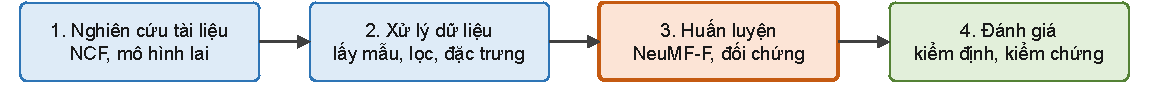
\includegraphics[width=1\textwidth]{media/figures/so_do/bc_09_cac_buoc.pdf}
    \caption{Các bước thực hiện đề tài}
    \label{fig:cac_buoc}
\end{figure}

\section{Ý nghĩa khoa học và thực tiễn của đề tài}
\label{sec:ynghia}

\subsection{Ý nghĩa khoa học}
\label{subsec:ynghia_khoahoc}

\begin{itemize}
    \item Đề tài xây dựng một mô hình lai giữa MF và DNN có bổ sung đặc trưng, và đánh giá nó trên dữ liệu giao dịch thời trang thực tế với kiểm định thống kê.
    \item Các mô hình đối chứng được thiết kế để tách riêng phần cải thiện do đặc trưng và phần do cách ghép hai nhánh. Cách thiết kế này cho phép xác định nhóm thông tin nào có giá trị nhất cho khuyến nghị thời trang.
    \item Quy trình đánh giá của đề tài tính đặc trưng không dùng thông tin tương lai, tinh chỉnh mọi mô hình với cùng ngân sách và lấy kết luận trên một mẫu khách hàng riêng. Quy trình này dùng lại được cho các nghiên cứu hệ thống khuyến nghị khác.
\end{itemize}

\subsection{Ý nghĩa thực tiễn}
\label{subsec:ynghia_thucte}

\begin{itemize}
    \item Mô hình chỉ dùng dữ liệu doanh nghiệp bán lẻ đã có: lịch sử giao dịch, danh mục sản phẩm, thông tin hội viên và doanh số theo ngày.
    \item Phân tích từng nhóm đặc trưng giúp doanh nghiệp biết nên ưu tiên cập nhật loại dữ liệu nào.
    \item Quy trình xử lý dữ liệu áp dụng được cho bộ dữ liệu thương mại điện tử khác, như đã làm với Amazon Beauty.
    \item Hệ thống demo cho phép so sánh trực quan các mô hình trên từng khách hàng.
\end{itemize}

\section{Bố cục của báo cáo}
\label{sec:bocuc}

Báo cáo gồm năm chương:
\begin{itemize}
    \item Chương~\ref{chap:tongquan} trình bày bối cảnh, câu hỏi nghiên cứu, mục tiêu, phạm vi, phương pháp và ý nghĩa của đề tài.
    \item Chương~\ref{chap:lythuyet} trình bày cơ sở lý thuyết về hệ thống khuyến nghị, nhân tử hoá ma trận, kiến trúc NeuMF, hợp nhất sớm và hợp nhất muộn, các độ đo đánh giá và các nghiên cứu liên quan.
    \item Chương~\ref{chap:thietke_trienkhai} trình bày dữ liệu, mô hình NeuMF-F, các mô hình đối chứng, cách huấn luyện, quy trình đánh giá và hệ thống demo.
    \item Chương~\ref{chap:thucnghiem} trình bày kết quả thực nghiệm trên H\&M và Amazon Beauty, rồi trả lời ba câu hỏi nghiên cứu.
    \item Chương~\ref{chap:ketluan} tổng kết kết quả, nêu hạn chế và hướng phát triển của đề tài.
\end{itemize}

    \chapter{CƠ SỞ LÝ THUYẾT VÀ CÁC CÔNG TRÌNH LIÊN QUAN}
\label{chap:lythuyet}

\section{Tổng quan về hệ thống khuyến nghị}
\label{sec:tongquan_rs}

\subsection{Lọc nội dung, lọc cộng tác và lọc lai}
\label{subsec:khainiem_rs}

Hệ thống khuyến nghị có ba hướng tiếp cận chính, khác nhau ở loại thông tin được dùng.
\begin{itemize}
    \item Lọc dựa trên nội dung (\textit{content-based filtering}) dùng thông tin của sản phẩm. Khách vừa mua một chiếc áo len sẽ được khuyến nghị những mẫu có loại hàng, nhóm hàng hay mô tả gần với chiếc áo đó.
    \item Lọc cộng tác (\textit{collaborative filtering}, CF) dùng hành vi mua của nhiều khách. Nếu nhiều người mua chung hai mẫu quần, khách mua mẫu thứ nhất có thể cũng quan tâm mẫu thứ hai. Cách này cần đủ lượt mua, nên hoạt động kém khi dữ liệu thưa.
    \item Lọc lai (\textit{hybrid filtering}) dùng cả hai nguồn thông tin để bù cho nhau.
\end{itemize}

Trước khi có học sâu, hệ thống khuyến nghị lai được ghép từ các kỹ thuật truyền thống. \textcite{burke2002hybrid} phân loại bảy cách lai:
\begin{itemize}
    \item Lai có trọng số (\textit{weighted}): cộng có trọng số điểm của nhiều kỹ thuật.
    \item Lai chuyển đổi (\textit{switching}): chọn một kỹ thuật tuỳ tình huống.
    \item Lai hỗn hợp (\textit{mixed}): trình bày đồng thời khuyến nghị của nhiều kỹ thuật.
    \item Kết hợp đặc trưng (\textit{feature combination}): dùng dữ liệu của kỹ thuật này làm đặc trưng cho kỹ thuật kia.
    \item Lai phân tầng (\textit{cascade}): kỹ thuật sau tinh chỉnh kết quả của kỹ thuật trước.
    \item Tăng cường đặc trưng (\textit{feature augmentation}): đầu ra của kỹ thuật này làm đầu vào cho kỹ thuật kia.
    \item Lai mức mô hình (\textit{meta-level}): mô hình học được của kỹ thuật này làm đầu vào cho kỹ thuật kia.
\end{itemize}

Dựa trên phân loại này, luận án của \textcite{holinh2023multisource} xây dựng một mô hình lai gồm ba thành phần, có điểm được tổng hợp qua một mạng truyền thẳng:
\begin{itemize}
    \item Lọc nội dung.
    \item Lọc cộng tác theo người dùng (UserKNN).
    \item Lọc cộng tác theo sản phẩm (ItemKNN).
\end{itemize}

Đề tài dùng lại ý tưởng này làm mô hình đối chứng Hybrid-CBCF, với hàm mục tiêu học theo cặp cho phản hồi ẩn. So sánh NeuMF-F với Hybrid-CBCF cho biết hợp nhất bằng mạng lưới thần kinh có hơn việc ghép điểm của các kỹ thuật truyền thống hay không.

Đề tài chọn hướng lai vì ba đặc điểm của dữ liệu H\&M:
\begin{itemize}
    \item Lịch sử mua dài hai năm, đủ để lọc cộng tác học sở thích của khách mua thường xuyên.
    \item Danh mục thời trang thay đổi liên tục và nhiều sản phẩm có ít lượt mua, nên lọc cộng tác chỉ dùng mã ID khó khuyến nghị tốt các sản phẩm này.
    \item Bộ dữ liệu có sẵn mô tả văn bản, nhóm hàng và doanh số theo ngày.
\end{itemize}

Vì vậy, mô hình của đề tài lấy lọc cộng tác (nhân tử hoá ma trận kết hợp mạng lưới thần kinh sâu) làm lõi, rồi bổ sung đặc trưng nội dung và thời gian.

\subsection{Lọc cộng tác dựa trên bộ nhớ và dựa trên mô hình}
\label{subsec:memory_model_based}

Theo cách khai thác dữ liệu tương tác, lọc cộng tác chia thành hai nhánh.

Nhánh dựa trên bộ nhớ (\textit{memory-based}) giữ nguyên ma trận tương tác và so trực tiếp các hàng hoặc các cột của nó. Hai khách được coi là giống nhau nếu đã mua nhiều sản phẩm chung, và hai sản phẩm giống nhau nếu có nhiều người cùng mua. Cách làm này không có tham số nào phải học. Với lọc cộng tác theo sản phẩm (ItemKNN) \parencite{sarwar2001item}, độ tương đồng cosine giữa hai sản phẩm $i$ và $j$ được tính trên vector cột tương tác của chúng:
\begin{equation}
    \text{sim}(i, j) = \cos(\vec{i}, \vec{j}) = \frac{\vec{i} \cdot \vec{j}}{\lVert \vec{i} \rVert \, \lVert \vec{j} \rVert}
    \label{eq:cosine_sim}
\end{equation}
Với phản hồi ẩn nhị phân, điểm của sản phẩm $i$ đối với người dùng $u$ là tổng độ tương đồng giữa $i$ và các sản phẩm $u$ đã mua, chỉ xét $k$ láng giềng gần nhất (\textit{nearest neighbors}) $\mathcal{N}_k(i)$ của $i$:
\begin{equation}
    \hat{y}_{ui} = \sum_{j \in \mathcal{N}_k(i) \cap \mathcal{I}_u} \text{sim}(i, j)
    \label{eq:itemcf_predict}
\end{equation}
Lọc cộng tác theo người dùng (UserKNN) làm đối xứng. Mô hình tìm $k$ người dùng có lịch sử mua giống $u$ nhất, ký hiệu $\mathcal{N}_k(u)$, rồi tính điểm mỗi sản phẩm bằng tổng độ tương đồng của các láng giềng đã mua sản phẩm đó:
\begin{equation}
    \hat{y}_{ui} = \sum_{v \in \mathcal{N}_k(u)} \text{sim}(u, v)\, y_{vi}
    \label{eq:usercf_predict}
\end{equation}
Với dữ liệu mua hàng, độ tương đồng cosine thường được tính trên vector mua nhị phân. Mẫu số được cộng thêm hệ số co (\textit{shrinkage}) $\lambda$ để giảm trọng số của các cặp có quá ít tương tác chung: $\text{sim}(a, b) = |\mathcal{I}_a \cap \mathcal{I}_b| / (\sqrt{|\mathcal{I}_a|\,|\mathcal{I}_b|} + \lambda)$, với $\mathcal{I}_a$ là tập sản phẩm $a$ đã mua (hoặc tập người dùng đã mua sản phẩm $a$). Mỗi hàng của ma trận tương đồng chỉ giữ $k$ láng giềng và được lưu dưới dạng ma trận thưa.

Nhánh dựa trên bộ nhớ có ưu điểm và nhược điểm sau:
\begin{itemize}
    \item Ưu điểm: đơn giản, không cần huấn luyện và dễ giải thích, vì chỉ ra được người dùng hay sản phẩm nào dẫn tới một khuyến nghị.
    \item Nhược điểm: ma trận tương đồng đầy đủ tăng theo bình phương số đối tượng, và chất lượng giảm khi dữ liệu quá thưa.
\end{itemize}

Nhánh dựa trên mô hình (\textit{model-based}) không giữ cả ma trận mà học một hàm có tham số, chẳng hạn nhân tử hoá ma trận hay mạng lưới thần kinh, để tóm tắt mỗi khách và mỗi sản phẩm bằng một vector ngắn. Vì mỗi đối tượng chỉ còn vài chục con số thay cho hàng nghìn ô của ma trận, mô hình vẫn chấm điểm được những cặp chưa từng xuất hiện, và chi phí huấn luyện chỉ tăng tuyến tính theo số tương tác. Nhân tử hoá ma trận và các mô hình dùng mạng lưới thần kinh như NeuMF đều thuộc nhánh này.

\subsection{Phản hồi ẩn}
\label{subsec:feedback_types}

Thông tin về sở thích của người dùng có hai dạng:
\begin{itemize}
    \item Phản hồi tường minh (\textit{explicit feedback}): người dùng tự nêu mức yêu thích, ví dụ chấm sao cho một bộ phim.
    \item Phản hồi ẩn (\textit{implicit feedback}): suy ra từ hành vi như mua, xem hay bấm vào sản phẩm.
\end{itemize}

Tệp giao dịch H\&M không có điểm đánh giá, chỉ có các giao dịch đã xảy ra. Vì vậy đề tài dùng phản hồi ẩn dạng nhị phân, lấy từ sự kiện mua hàng:
\begin{equation}
    y_{ui} = \begin{cases}
        1, & \text{nếu người dùng } u \text{ đã mua sản phẩm } i \\
        0, & \text{ngược lại}
    \end{cases}
    \label{eq:implicit_binary}
\end{equation}
Nhãn $y_{ui} = 1$ chỉ xác nhận khách đã mua, không xác nhận khách hài lòng. Nhãn $y_{ui} = 0$ có thể nghĩa là khách chưa biết đến sản phẩm, không nhất thiết là không thích. Do đó các cặp chưa tương tác không thể coi là nhãn âm chắc chắn, và kỹ thuật lấy mẫu âm phải được thiết kế cẩn thận.

\subsection{Độ thưa dữ liệu và vấn đề \textit{cold start}}
\label{subsec:thachthuc_sparsity}

Lọc cộng tác có hai thách thức chính:
\begin{itemize}
    \item Độ thưa dữ liệu. Mỗi khách chỉ mua một phần rất nhỏ trong hàng nghìn sản phẩm, nên gần như mọi ô của ma trận $M \times N$ đều trống. Lọc $k$-core (chỉ giữ khách và sản phẩm có ít nhất $k$ lượt mua) làm giảm độ thưa, nhưng ma trận vẫn rất thưa.
    \item Khởi đầu lạnh (\textit{cold start}). Khách vừa đăng ký hoặc sản phẩm vừa lên kệ chưa có lượt mua nào, nên lọc cộng tác không có dữ liệu để học vector cho chúng. Những đối tượng chỉ có ít lượt mua gặp dạng nhẹ hơn của vấn đề này: vector mã ID của chúng kém tin cậy.
\end{itemize}

Đề tài bổ sung đặc trưng nội dung và ngữ cảnh vào mô hình lai chủ yếu để giảm ảnh hưởng của hai thách thức này.

\section{Lọc cộng tác và nhân tử hoá ma trận}
\label{sec:cf_mf}

\subsection{Mô hình nhân tử hoá ma trận}
\label{subsec:mf_model}

Ý tưởng của nhân tử hoá ma trận \parencite{koren2009matrix} là mô tả mỗi người dùng và mỗi sản phẩm bằng $d$ con số, với $d \ll \min(M, N)$. Có thể hình dung mỗi chiều như một ``khẩu vị'' ẩn, chẳng hạn thiên về đồ thể thao hay đồ công sở, dù mô hình không đặt tên cho các chiều này. Người dùng $u$ ứng với vector $p_u \in \mathbb{R}^d$, sản phẩm $i$ ứng với $q_i \in \mathbb{R}^d$, và điểm dự đoán là tích vô hướng của hai vector:
\begin{equation}
    \hat{y}_{ui} = p_u^T q_i = \sum_{f=1}^{d} p_{uf} q_{if}
    \label{eq:mf_dot}
\end{equation}
Các biến thể của MF khác nhau ở cách học hai ma trận $P$ và $Q$. Phân tích giá trị suy biến (\textit{singular value decomposition}, SVD) cổ điển cần ma trận đầy đủ, vì vậy không áp dụng trực tiếp được cho ma trận tương tác thưa, nơi phần lớn ô chưa được quan sát. Các biến thể dùng trong hệ thống khuyến nghị thay vào đó tối ưu sai số trên các ô đã biết, kèm điều chuẩn (\textit{regularization}). Với phản hồi ẩn, BPR tối ưu trực tiếp thứ hạng theo cặp, và đề tài dùng BPR-MF làm mô hình đối chứng MF chính.

\subsection{Hạn chế của tích vô hướng}
\label{subsec:mf_limitations}

Tích vô hướng kết hợp các chiều ẩn theo dạng tuyến tính. Các tác giả của kiến trúc lọc cộng tác bằng mạng lưới thần kinh (\textit{neural collaborative filtering}, NCF) cho rằng vì lý do đó phép toán này không học được tương tác phi tuyến giữa các chiều ẩn của người dùng và sản phẩm. Lập luận này là động cơ của kiến trúc NCF. Việc bổ sung thành phần phi tuyến có thực sự cải thiện chất lượng khuyến nghị hay không phụ thuộc vào dữ liệu, và được đề tài kiểm tra bằng thực nghiệm trên dữ liệu H\&M.

\subsection{Tối ưu thứ hạng theo cặp: BPR}
\label{subsec:bpr}

MF, GMF và MLP được huấn luyện như một bài toán phân loại, trong đó mỗi cặp $(u, i)$ được chấm riêng thành $\hat{y}_{ui}$ rồi so với nhãn 0 hoặc 1. Trong khi đó, hệ thống khuyến nghị chỉ cần xếp đúng thứ tự: món khách sẽ mua phải đứng trên món khách không mua. Bayesian Personalized Ranking (BPR) \parencite{rendle2009bpr} huấn luyện thẳng theo yêu cầu này, với giả định người dùng thích một sản phẩm đã tương tác $i$ hơn một sản phẩm chưa tương tác $j$. Với mỗi bộ ba $(u, i, j)$ trong đó $i \in \mathcal{I}_u$ và $j \notin \mathcal{I}_u$, hàm mất mát BPR là:
\begin{equation}
    \mathcal{L}_{BPR} = -\sum_{(u,i,j) \in \mathcal{D}_S} \ln \sigma\left(\hat{y}_{ui} - \hat{y}_{uj}\right) + \lambda_\Theta \lVert \Theta \rVert^2
    \label{eq:bpr_loss}
\end{equation}
trong đó $\mathcal{D}_S$ là tập các bộ ba được lấy mẫu. Khi $\hat{y}_{ui}$ được tính theo Công thức~\eqref{eq:mf_dot}, ta có mô hình BPR-MF, một mô hình đối chứng của đề tài. Mục tiêu theo cặp của BPR sát với bài toán xếp hạng Top-$K$ hơn hàm mất mát theo từng điểm, nhưng BPR-MF vẫn là mô hình tuyến tính.

\section{Kiến trúc lọc cộng tác bằng mạng lưới thần kinh (NCF)}
\label{sec:ncf_architecture}

Kiến trúc NCF do \textcite{he2017ncf} đề xuất gồm hai mô hình thành phần, GMF và MLP, và mô hình hợp nhất của chúng, NeuMF.

\subsection{Generalized Matrix Factorization (GMF)}
\label{subsec:gmf}

GMF viết lại MF dưới dạng một mạng lưới thần kinh. Thay vì cộng ngay các tích $p_{uf} q_{if}$ như Công thức~\eqref{eq:mf_dot}, GMF giữ chúng thành một vector bằng phép nhân từng phần tử (tích Hadamard, ký hiệu $\odot$) giữa vector nhúng của người dùng $p_u^G$ và của sản phẩm $q_i^G$:
\begin{equation}
    \phi^{GMF} = p_u^G \odot q_i^G
    \label{eq:gmf_hadamard}
\end{equation}
\begin{equation}
    \hat{y}_{ui}^{GMF} = \sigma \left( h^T \phi^{GMF} \right) = \sigma \left( h^T (p_u^G \odot q_i^G) \right)
    \label{eq:gmf_predict}
\end{equation}
trong đó $h$ là vector trọng số của lớp đầu ra và $\sigma(x) = 1 / (1 + e^{-x})$ là hàm sigmoid. Nếu mọi phần tử của $h$ bằng 1 và bỏ hàm sigmoid, GMF trở về đúng MF. Khi $h$ được học, mỗi chiều ẩn có trọng số riêng.

\subsection{Multi-Layer Perceptron (MLP)}
\label{subsec:mlp}

Nhánh MLP nối vector nhúng $p_u^M$ và $q_i^M$ thành đầu vào của một chuỗi lớp ẩn:
\begin{equation}
    z_1 = \phi_1^{MLP} = \begin{bmatrix} p_u^M \\ q_i^M \end{bmatrix}
    \label{eq:mlp_concat}
\end{equation}
\begin{equation}
    \phi_L^{MLP} = a_L \left( W_L^T \phi_{L-1}^{MLP} + b_L \right)
    \label{eq:mlp_layerL}
\end{equation}
trong đó $W_L$, $b_L$ và $a_L$ lần lượt là ma trận trọng số, vector độ lệch (\textit{bias}) và hàm kích hoạt phi tuyến (ví dụ ReLU) của lớp thứ $L$. Cấu trúc này cho phép mô hình học tương tác phi tuyến giữa biểu diễn của người dùng và của sản phẩm.

\subsection{Mô hình lai NeuMF}
\label{subsec:neumf_arch}

NeuMF ghép song song nhánh tuyến tính GMF và nhánh phi tuyến MLP trước lớp dự đoán:
\begin{equation}
    \phi^{NeuMF} = \begin{bmatrix} \phi^{GMF} \\ \phi_L^{MLP} \end{bmatrix} = \begin{bmatrix} p_u^G \odot q_i^G \\ \phi_L^{MLP} \end{bmatrix}
    \label{eq:neumf_concat}
\end{equation}
\begin{equation}
    \hat{y}_{ui} = \sigma \left( h^T \begin{bmatrix} p_u^G \odot q_i^G \\ \phi_L^{MLP} \end{bmatrix} \right)
    \label{eq:neumf_prediction}
\end{equation}
Chữ ``lai'' trong tên đề tài trước hết chỉ việc kết hợp hai cách mô hình hoá tương tác, nhân tử hoá ma trận (tuyến tính) và mạng lưới thần kinh sâu (phi tuyến), trong cùng một mô hình. Vì hai nhánh được ghép ngay ở mức biểu diễn, trước lớp dự đoán, NeuMF là một mô hình hợp nhất sớm. Mô hình đề xuất NeuMF-F giữ cấu trúc này và bổ sung đặc trưng sản phẩm, khách hàng và thời gian vào vector của cả hai nhánh. Vì kết hợp lọc cộng tác với thông tin nội dung, NeuMF-F cũng là một hệ thống khuyến nghị lai theo nghĩa rộng.

Hình~\ref{fig:neumf_architecture} vẽ kiến trúc NeuMF theo cách trình bày của bài báo gốc:
\begin{itemize}
    \item Người dùng và sản phẩm được mã hoá one-hot.
    \item Mỗi nhánh có bộ vector nhúng riêng: màu xanh cho GMF, màu tím cho MLP.
    \item Hai nhánh gặp nhau ở lớp hợp nhất trước khi qua hàm sigmoid.
    \item Hai nhánh dùng cùng $d$, và chuỗi lớp ẩn của MLP, thường gọi là tháp (\textit{tower}), giảm một nửa số chiều qua mỗi lớp như cấu hình gốc của NCF.
\end{itemize}

\begin{figure}[H]
    \centering
    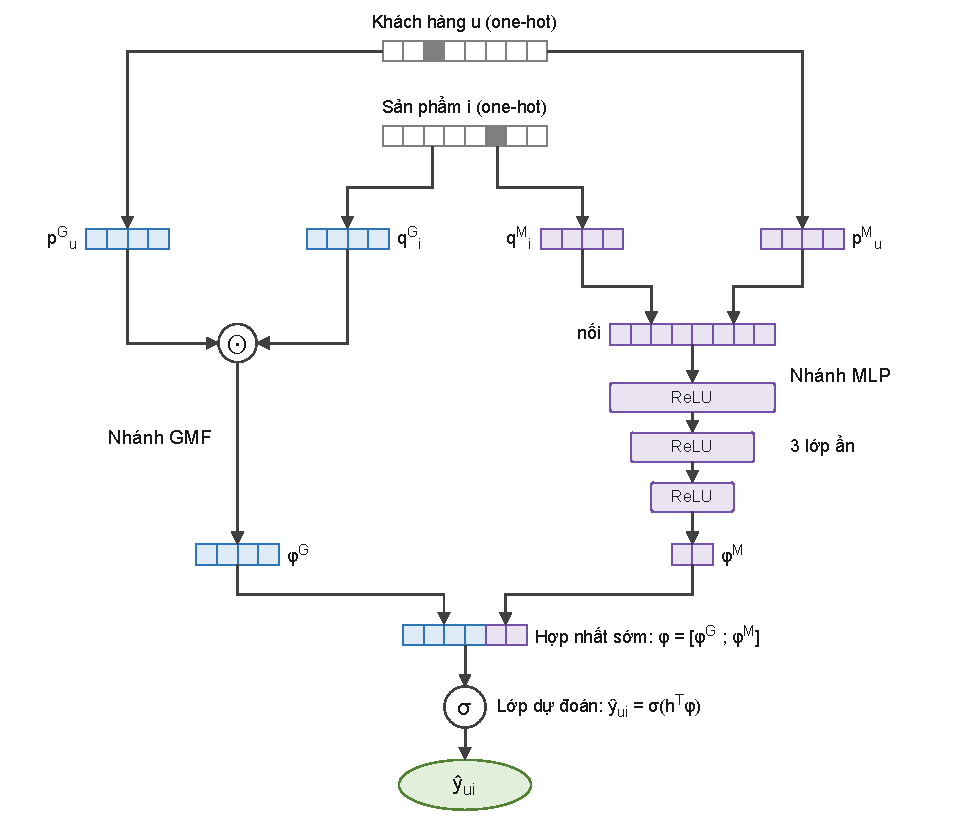
\includegraphics[width=0.95\textwidth]{media/figures/so_do/bc_07_kien_truc_neumf.pdf}
    \caption{Kiến trúc NeuMF}
    \label{fig:neumf_architecture}
\end{figure}

\subsection{Hợp nhất sớm và hợp nhất muộn}
\label{subsec:early_late_fusion}

Khi hệ thống khuyến nghị kết hợp nhiều nguồn thông tin, hay nhiều góc nhìn về người dùng và sản phẩm, có hai cách hợp nhất cơ bản. Hai cách này khác nhau ở mức diễn ra phép hợp nhất \parencite{holinh2023multisource}.
\begin{itemize}
    \item Hợp nhất sớm (\textit{early fusion}) diễn ra ở mức đặc trưng hoặc biểu diễn. Các vector $v_1, \dots, v_m$ của từng góc nhìn được nối thành một biểu diễn chung, rồi một mô hình $h$ duy nhất học tương tác giữa chúng và đưa ra dự đoán:
    \begin{equation}
        p = h\big([v_1;\, v_2;\, \dots;\, v_m]\big)
        \label{eq:early_fusion}
    \end{equation}
    \item Hợp nhất muộn (\textit{late fusion}) diễn ra ở mức điểm dự đoán. Mỗi góc nhìn được xử lý bởi một mô hình riêng $h_j$, rồi các dự đoán được kết hợp bằng một cơ chế $F$, như lấy trung bình, bỏ phiếu, trọng số cố định hoặc một mô hình học:
    \begin{equation}
        p = F\big(h_1(v_1),\, h_2(v_2),\, \dots,\, h_m(v_m)\big)
        \label{eq:late_fusion}
    \end{equation}
    Khi $F$ là tổng có trọng số, đây chính là cách lai có trọng số trong phân loại của Burke. Mô hình lai ở chương 3 luận án thuộc loại này, và mô hình đối chứng Hybrid-CBCF của đề tài cũng vậy. Ở hai mô hình này, $F$ là bỏ phiếu hoặc tổng có trọng số của điểm từ ba mô hình truyền thống.
\end{itemize}

Ưu điểm của hợp nhất sớm là học được tương tác giữa các nguồn thông tin, nhưng nó đòi hỏi một mô hình phù hợp với mọi nguồn. Hợp nhất muộn linh hoạt hơn, song chỉ làm việc trên kết quả dự đoán nên không nắm được tương tác đó.

Trong đề tài, hai góc nhìn chính là hai cách mô hình hoá tương tác: góc nhìn tuyến tính của nhánh MF (vector $p_u^G \odot q_i^G$ của GMF) và góc nhìn phi tuyến của nhánh DNN (vector cuối $\phi_L^{MLP}$ của MLP). NeuMF nối hai vector này rồi đưa qua một lớp dự đoán chung (Công thức~\eqref{eq:neumf_concat}, \eqref{eq:neumf_prediction}). Đây là hợp nhất sớm ở mức biểu diễn, và cả mạng được huấn luyện chung từ đầu đến cuối, như phần (a) của Hình~\ref{fig:fusion_compare}. Mô hình đề xuất của đề tài giữ cách hợp nhất này. Ngoài ra, đặc trưng nội dung và ngữ cảnh được cộng vào vector của từng nhánh ngay ở đầu vào, do đó cũng được hợp nhất sớm với thông tin cộng tác.

Hợp nhất muộn tương ứng là trộn điểm của hai mô hình MF và DNN được huấn luyện riêng:
\begin{equation}
    \hat{y}_{ui} = w\,\tilde{s}^{MF}_{ui} + (1-w)\,\tilde{s}^{DNN}_{ui}, \qquad
    \tilde{s}_{ui} = \frac{s_{ui} - \min_{j \in \mathcal{C}_u} s_{uj}}{\max_{j \in \mathcal{C}_u} s_{uj} - \min_{j \in \mathcal{C}_u} s_{uj}}
    \label{eq:late_fusion_mfdnn}
\end{equation}
trong đó điểm $s_{ui}$ của mỗi mô hình được chuẩn hoá min--max trên tập ứng viên $\mathcal{C}_u$ để hai thang điểm so sánh được. Tập ứng viên là các sản phẩm được đem ra xếp hạng cho người dùng $u$. Trọng số $w \in [0, 1]$ được chọn trên tập xác thực. Với $w = 1$ hoặc $w = 0$, thứ hạng trùng với thứ hạng của từng thành phần. Trong đề tài, mô hình hợp nhất muộn LateFusion-F trộn điểm của hai nhánh có đặc trưng được huấn luyện riêng, như phần (b) của Hình~\ref{fig:fusion_compare}. Riêng nhánh MLP khi đứng một mình chỉ nối vector người dùng và sản phẩm ở đầu vào. Đó là một mô hình DNN thuần, chưa có phần MF.

\begin{figure}[H]
    \centering
    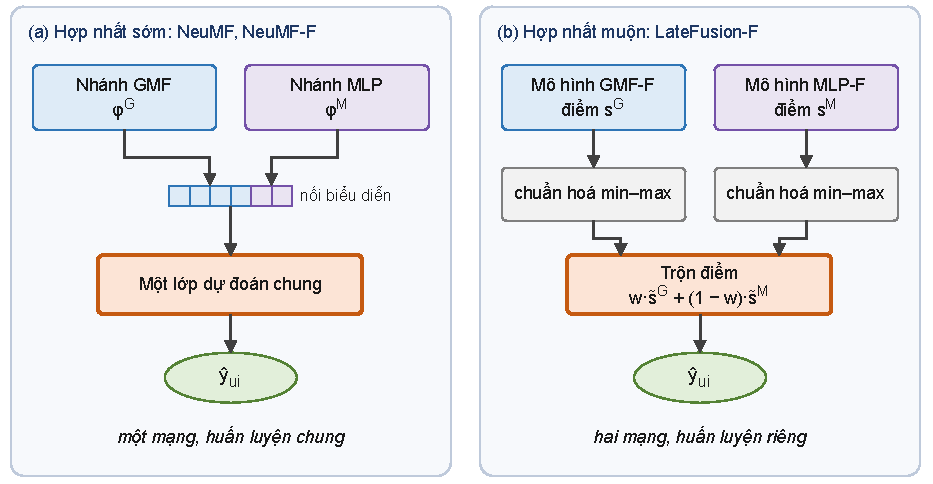
\includegraphics[width=0.95\textwidth]{media/figures/so_do/bc_08_hop_nhat.pdf}
    \caption{Hợp nhất sớm và hợp nhất muộn}
    \label{fig:fusion_compare}
\end{figure}

\subsection{Lấy mẫu âm và hàm mất mát entropy chéo nhị phân}
\label{subsec:negative_sampling_loss}

Dữ liệu mua hàng chỉ cho biết khách đã mua gì, vì vậy chỉ có nhãn dương ($y_{ui} = 1$). Để mô hình học được cả chiều ngược lại, NCF lấy mẫu âm (\textit{negative sampling}): với mỗi lượt mua, chọn ngẫu nhiên vài sản phẩm khách chưa mua và tạm coi là nhãn âm ($y_{ui} = 0$). Mô hình sau đó được huấn luyện như một bộ phân loại nhị phân, với hàm mất mát entropy chéo nhị phân (\textit{binary cross-entropy}, BCE):
\begin{equation}
    \mathcal{L}_{BCE} = -\sum_{(u, i) \in \mathcal{Y} \cup \mathcal{Y}^-} \left[ y_{ui} \log \hat{y}_{ui} + (1 - y_{ui}) \log (1 - \hat{y}_{ui}) \right]
    \label{eq:bce_loss}
\end{equation}
trong đó $\mathcal{Y}$ là tập tương tác dương và $\mathcal{Y}^-$ là tập cặp âm được lấy mẫu.

\section{Mô hình lai dựa trên đặc trưng}
\label{sec:modern_trends}

\subsection{Bổ sung đặc trưng vào mô hình lai}
\label{subsec:deep_ctr}

Một cách khắc phục hạn chế về thông tin của MF là cho mô hình học từ cả đặc trưng, không chỉ từ mã ID. Các mô hình tiêu biểu theo hướng này gồm:
\begin{itemize}
    \item Factorization Machines (FM) \parencite{rendle2010fm}: mỗi đặc trưng có một vector ẩn, và mức độ hai đặc trưng hợp nhau được đo bằng tích vô hướng của hai vector đó. Khi chỉ có mã khách hàng và mã sản phẩm, FM trở về MF.
    \item Wide \& Deep \parencite{cheng2016wide} và DeepFM \parencite{guo2017deepfm}: ghép một thành phần tuyến tính với một mạng MLP trên đầu vào có đặc trưng. Cấu trúc này gần giống NeuMF, chỉ khác ở đầu vào.
\end{itemize}

NeuMF-F đi theo hướng này. Mô hình giữ hai nhánh GMF và MLP, nhưng biểu diễn mỗi khách hàng và sản phẩm bằng vector nhúng mã ID cộng với phép chiếu tuyến tính của đặc trưng.

Khi mô hình nhận cả mã ID và đặc trưng, nó có thể dựa hẳn vào mã ID mà bỏ qua đặc trưng. DropoutNet \parencite{volkovs2017dropoutnet} xử lý điều này bằng cách bỏ ngẫu nhiên vector ID khi huấn luyện, buộc mô hình học chấm điểm từ đặc trưng. Kỹ thuật này hữu ích khi muốn mô hình chấm được cả những sản phẩm có ít hoặc chưa có lượt mua.

Văn bản của sản phẩm (tên, mô tả) được biểu diễn bằng TF-IDF \parencite{salton1988term}. Một từ có trọng số cao với một sản phẩm khi nó lặp lại trong mô tả của sản phẩm đó nhưng ít gặp trong cả danh mục. Ma trận TF-IDF sau đó được giảm chiều bằng phân tích giá trị suy biến rút gọn (\textit{truncated SVD}) \parencite{deerwester1990lsa}. Nhờ bước này, các mô tả cùng chủ đề nhưng dùng từ khác nhau có vector gần nhau. Cách biểu diễn này không cần dữ liệu tương tác và tính nhanh.

\subsection{Lý do chọn kiến trúc hai nhánh}
\label{subsec:other_trends}

Ngoài mô hình lai dựa trên đặc trưng, hệ thống khuyến nghị còn có các hướng như mô hình theo chuỗi hành vi, mô hình trên đồ thị tương tác và mô hình ngôn ngữ lớn. Đề tài chọn kiến trúc hai nhánh của NeuMF vì ba lý do:
\begin{itemize}
    \item Về dữ liệu: giao dịch H\&M chỉ ghi ngày mua, không có giờ hay mã phiên, nên khó áp dụng mô hình chuỗi. Bộ dữ liệu lại có thuộc tính và mô tả sản phẩm, phù hợp với cách biểu diễn ``vector nhúng ID cộng đặc trưng''.
    \item Về mục tiêu: hai nhánh tách biệt cho phép đo riêng đóng góp của đặc trưng và của cách hợp nhất.
    \item Về tài nguyên: mô hình đồ thị và mô hình ngôn ngữ lớn cần nhiều tài nguyên tính toán hơn mức đề tài có.
\end{itemize}

\section{Các độ đo đánh giá Top-K}
\label{sec:metrics}

Với mỗi người dùng được đánh giá $u$, mô hình xếp hạng tập ứng viên $\mathcal{C}_u$ và trả về danh sách $\text{Rec}_K(u)$ gồm $K$ sản phẩm đầu. Gọi $T_u$ là tập sản phẩm mục tiêu của $u$ và $\text{hits}_u = |T_u \cap \text{Rec}_K(u)|$. Khi chia dữ liệu theo một mốc thời gian chung như trong đề tài, một người dùng có thể có nhiều sản phẩm mục tiêu. Mọi độ đo được tính cho từng người dùng rồi lấy trung bình trên tập người dùng được đánh giá $\mathcal{U}_{test}$.

Hit Ratio (HR@K) là độ đo đơn giản nhất. Nó kiểm tra trong $K$ khuyến nghị có ít nhất một món khách thật sự mua hay không. Mỗi người dùng được tính 1 nếu có và 0 nếu không:
\begin{equation}
    \text{HR@K} = \frac{1}{|\mathcal{U}_{test}|} \sum_{u \in \mathcal{U}_{test}} \mathbb{I}\left( \text{hits}_u \ge 1 \right)
    \label{eq:hr_k}
\end{equation}

Precision@K là tỉ lệ khuyến nghị đúng trong $K$ khuyến nghị, đo độ chính xác từ phía danh sách. Recall@K là tỉ lệ các món khách thật sự mua đã có mặt trong danh sách, đo độ bao phủ từ phía khách:
\begin{equation}
    \text{Precision@K}(u) = \frac{\text{hits}_u}{K}, \qquad \text{Recall@K}(u) = \frac{\text{hits}_u}{|T_u|}
    \label{eq:precision_recall}
\end{equation}
Khi $|T_u| = 1$, Recall@K trùng HR@K và Precision@K bằng HR@K chia cho $K$. Hai độ đo này chỉ mang thông tin riêng khi người dùng có nhiều sản phẩm mục tiêu.

Ba độ đo trên không phân biệt món đúng nằm ở vị trí đầu hay vị trí thứ $K$, trong khi người dùng thường chỉ xem vài khuyến nghị đầu. NDCG@K (\textit{normalized discounted cumulative gain}) tính đến vị trí bằng cách giảm dần đóng góp của một món đúng khi nó nằm càng xa đầu danh sách. Với mức liên quan nhị phân, định nghĩa của \textcite{jarvelin2002} là:
\begin{equation}
    \begin{aligned}
        \text{NDCG@K}(u) &= \frac{\text{DCG@K}(u)}{\text{IDCG@K}(u)}, \\
        \text{DCG@K}(u) &= \sum_{j=1}^{K} \frac{\mathbb{I}(\text{Rec}_K(u)_j \in T_u)}{\log_2(j + 1)}, \\
        \text{IDCG@K}(u) &= \sum_{j=1}^{\min(|T_u|, K)} \frac{1}{\log_2(j + 1)}
    \end{aligned}
    \label{eq:ndcg_k}
\end{equation}
IDCG là giá trị DCG khi mọi sản phẩm mục tiêu xếp ở đầu danh sách, nên NDCG@K nằm trong $[0, 1]$. Với $|T_u| = 1$ và sản phẩm mục tiêu ở hạng $r$, NDCG@K bằng $1/\log_2(r+1)$ nếu $r \le K$ và bằng 0 nếu ngược lại.

\subsection{Xếp hạng toàn bộ và xếp hạng trên tập lấy mẫu}

Một số công trình, trong đó có NCF, đánh giá bằng cách xếp sản phẩm mục tiêu giữa một tập nhỏ ứng viên lấy mẫu, cụ thể là sản phẩm kiểm thử cùng 100 sản phẩm người dùng chưa tương tác. \textcite{krichene2020sampled} chứng minh độ đo trên tập ứng viên lấy mẫu không nhất quán với độ đo trên toàn bộ danh mục, thậm chí có thể đảo ngược kết luận ``A tốt hơn B'', và đề nghị không lấy mẫu. Đề tài vì vậy chỉ dùng cách xếp hạng toàn bộ (\textit{full ranking}). Mỗi người dùng được xếp hạng trên toàn bộ tập ứng viên, trừ sản phẩm đã mua. Ở tập kiểm thử (\textit{test set}) của mẫu kiểm định, tập này có khoảng \VData{Btest}{cand} sản phẩm.

\subsection{Độ đo ngoài độ chính xác}
\label{subsec:beyond_accuracy}

Một mô hình chỉ khuyến nghị những món bán chạy nhất vẫn có thể đạt HR@K khá, vì món bán chạy dễ trúng, nhưng danh sách của nó gần như giống nhau với mọi khách. Để mô tả danh sách khuyến nghị ngoài độ chính xác, đề tài dùng độ phủ (\textit{coverage}): tỉ lệ sản phẩm của không gian ứng viên $\mathcal{I}_{cand}$ xuất hiện trong danh sách khuyến nghị của ít nhất một người dùng:
\begin{equation}
    \text{Coverage@K} = \frac{\left| \bigcup_{u \in \mathcal{U}_{test}} \text{Rec}_K(u) \right|}{|\mathcal{I}_{cand}|}
    \label{eq:coverage}
\end{equation}
Độ phủ thấp cho thấy mô hình chỉ dùng một phần nhỏ danh mục. Trường hợp giới hạn là Most Popular, khi mọi người dùng nhận gần như cùng một danh sách. Độ đo này chỉ mang tính mô tả.

\section{Ba nghiên cứu nền tảng}
\label{sec:related_work}
\label{subsec:foundation_studies}

Đề tài chọn ba nghiên cứu làm nền tảng tham chiếu vì chúng liên quan trực tiếp tới mô hình và cách đánh giá:
\begin{itemize}
    \item \textcite{he2017ncf} đề xuất kiến trúc NeuMF mà NeuMF-F kế thừa.
    \item \textcite{rendle2020ncfmf} kiểm tra lại liệu NeuMF có tốt hơn MF được tinh chỉnh kỹ hay không, câu hỏi mà đề tài đặt lại trên dữ liệu H\&M.
    \item Luận án của \textcite{holinh2023multisource} hệ thống hoá hai cách hợp nhất sớm, muộn và việc bổ sung nguồn thông tin ngoài ma trận tương tác.
\end{itemize}

Bảng~\ref{tab:foundation_studies} đối chiếu thiết lập thực nghiệm của ba nghiên cứu với đề tài. Số liệu của mỗi nghiên cứu lấy từ bài gốc.

Các con số trong bảng không so sánh trực tiếp được với nhau:
\begin{itemize}
    \item Hai bài về NCF xếp sản phẩm mục tiêu giữa 101 ứng viên, nên HR@10 đạt khoảng 0,7 đến 0,9.
    \item Đề tài xếp hạng trên khoảng 6 đến 7 nghìn ứng viên, nên cùng độ đo cho giá trị thấp hơn nhiều.
    \item Luận án giải bài toán dự đoán điểm đánh giá với độ đo sai số, không xếp hạng.
\end{itemize}

Vì vậy chỉ nên đọc mức cải thiện tương đối so với đối chứng trong từng nghiên cứu. Từ ba nghiên cứu này, đề tài kế thừa kiến trúc và cách huấn luyện của NeuMF, yêu cầu tinh chỉnh đầy đủ mô hình đối chứng, và khung hợp nhất sớm, hợp nhất muộn.

\begingroup\small
\begin{xltabular}{\textwidth}{|>{\raggedright\arraybackslash}p{2.2cm}|>{\raggedright\arraybackslash}p{4.1cm}|>{\raggedright\arraybackslash}p{3.3cm}|>{\raggedright\arraybackslash}X|}
    \caption{Ba nghiên cứu nền tảng và thiết lập của đề tài}
    \label{tab:foundation_studies} \\
    \hline
    Nghiên cứu & Dữ liệu; bài toán và độ đo & Cách chia; tập ứng viên & Kết quả công bố (số liệu của bài gốc) \\
    \hline
    \endfirsthead
    \hline
    Nghiên cứu & Dữ liệu; bài toán và độ đo & Cách chia; tập ứng viên & Kết quả công bố (số liệu của bài gốc) \\
    \hline
    \endhead

    \endfoot
    He và cộng sự, 2017 & MovieLens 1M (6.040 người dùng, 3.706 phim, 1.000.209 tương tác) và Pinterest (55.187 người dùng, 9.916 sản phẩm, 1.500.809 tương tác), phản hồi ẩn. Xếp hạng Top-$K$; HR@10, NDCG@10 & Giữ lại tương tác mới nhất của mỗi người dùng làm kiểm thử. 101 ứng viên: sản phẩm kiểm thử và 100 sản phẩm chưa tương tác lấy ngẫu nhiên & NeuMF có tiền huấn luyện: MovieLens HR@10 = 0,730, NDCG@10 = 0,447 (64 nhân tố); Pinterest HR@10 = 0,880, NDCG@10 = 0,558 (16 nhân tố). Trung bình cao hơn eALS 4,5\% và BPR 4,9\% (tương đối). \\
    \hline
    Rendle và cộng sự, 2020 & Như NCF: MovieLens 1M và Pinterest; HR@10, NDCG@10 & Như NCF: giữ lại tương tác mới nhất; 101 ứng viên & MF tinh chỉnh kỹ: MovieLens 0,7294 / 0,4523, Pinterest 0,8895 / 0,5794 (HR@10 / NDCG@10); NeuMF trong bảng so sánh của bài: 0,7093 / 0,4349 và 0,8777 / 0,5576. MF cao hơn NeuMF 2,8\% HR@10 và 4,0\% NDCG@10 (MovieLens), 1,3\% và 3,9\% (Pinterest). \\
    \hline
    Hồ Thị Linh, 2023 & MovieLens (77.764 đánh giá, 27.042 người dùng, 8.203 phim); Amazon Electronics (85.065 đánh giá, 1.042 người dùng), Toys and Games (71.780; 5.462), Video Games (98.769; 2.291). Dự đoán điểm đánh giá; RMSE, MAE, Precision & Chia ngẫu nhiên 80\% huấn luyện (20\% trong đó để xác thực), 20\% kiểm thử. Không xếp hạng trên tập ứng viên & Hợp nhất sớm vector MF và đặc trưng văn bản qua mạng lưới thần kinh (chương 4), Electronics: RMSE 1,01, Precision 82,86\% so với SVD 1,16 và 69,55\% (RMSE giảm 12,93\%, Precision tăng 19,14\%). Transformer hợp nhất nhiều góc nhìn (chương 5), Toys and Games: MAE 0,445, RMSE 0,743, Precision 92,07\% so với SVD 0,844 / 1,120 / 68,06\%. \\
    \hline
    Đề tài, 2026 & H\&M, mẫu kiểm định (\VData{B}{nusers} khách, \VData{B}{nitems} sản phẩm, \VData{B}{nkeptpairs} cặp) và Amazon Beauty 5-core (\AData{all}{nusers} khách, \AData{all}{nitems} sản phẩm, \AData{all}{nkeptpairs} cặp), phản hồi ẩn. Xếp hạng Top-$K$; NDCG@10 (chính), Recall, HR, Precision ở $K = 10, 15, 20$ & Theo mốc thời gian chung; mẫu khách hàng độc lập (H\&M). Ứng viên: mọi sản phẩm đã có dữ liệu huấn luyện, trừ sản phẩm khách đã mua; trung bình \VData{Btest}{cand} (H\&M), \AData{test}{cand} (Amazon) & Mô hình đề xuất NeuMF-F và 13 mô hình đối chứng, cùng ngân sách tinh chỉnh; kiểm định Wilcoxon, bootstrap và hiệu chỉnh Holm \\ \hline
\end{xltabular}
\endgroup

\section{Khoảng trống nghiên cứu}
\label{sec:khoangtrong_nghiencuu}

Các nghiên cứu liên quan còn ba điểm chưa giải quyết:
\begin{itemize}
    \item Các nghiên cứu về NCF chủ yếu được đánh giá trên dữ liệu phim ảnh hoặc mạng xã hội hình ảnh, với cách giữ lại tương tác cuối và tập ứng viên lấy mẫu.
    \item Các nghiên cứu đánh giá lại cho thấy NeuMF chỉ dùng mã ID khó vượt các mô hình đơn giản được tinh chỉnh kỹ.
    \item Các mô hình dùng đặc trưng thường được đánh giá cho bài toán dự đoán nhấp chuột, không phải xếp hạng Top-$K$ trên toàn bộ danh mục.
\end{itemize}

Từ đó, đề tài tập trung vào hai việc:
\begin{itemize}
    \item Về mô hình: xây dựng NeuMF-F, giữ cấu trúc hai nhánh MF và DNN của NeuMF và dùng thêm đặc trưng của sản phẩm, khách hàng, thời gian.
    \item Về đánh giá: thử mô hình trên dữ liệu giao dịch thời trang thực tế với cách làm gần với khi triển khai.
    \begin{itemize}
        \item Dữ liệu được chia theo thời gian.
        \item Đặc trưng không dùng thông tin tương lai.
        \item Mọi mô hình được tinh chỉnh với cùng ngân sách và xếp hạng trên toàn bộ tập ứng viên.
        \item Kết luận được lấy trên một mẫu khách hàng không dùng để chọn cấu hình.
    \end{itemize}
\end{itemize}

\FloatBarrier

    \chapter{PHƯƠNG PHÁP NGHIÊN CỨU VÀ THIẾT KẾ MÔ HÌNH LAI NEUMF-F}
\label{chap:thietke_trienkhai}

Chương này trình bày phương pháp của đề tài theo đúng thứ tự thực hiện: dữ liệu, mô hình đề xuất và các mô hình đối chứng, huấn luyện, đánh giá, rồi suy luận và hệ thống demo. Điểm xuất phát là bộ dữ liệu H\&M với đặc điểm thưa và biến động theo thời gian, từ đó quyết định cách chia dữ liệu, cách tính đặc trưng và cách thiết lập tập ứng viên. Mô hình đề xuất NeuMF-F được xây trên nền kiến trúc NeuMF, giữ nguyên hai nhánh GMF và MLP, và bổ sung đặc trưng vào biểu diễn của cả hai nhánh. Để kết luận có thể tin cậy, quy trình đánh giá được thiết kế riêng với tập kiểm định độc lập, đăng ký trước và kiểm định thống kê. Các bước xử lý chính được viết thành mã giả.

\section{Quy trình tổng thể của hệ thống}
\label{sec:system_architecture}

Hệ thống được tổ chức theo trình tự một mô hình gợi ý đi qua khi đưa vào sử dụng: xây dựng đặc trưng, huấn luyện, lưu mô hình và suy luận (Hình~\ref{fig:system_architecture}). Chuỗi bước này được gọi là đường ống xử lý (\textit{pipeline}). Mỗi lần chạy, đường ống nhận một mốc thời gian $\tau$. Mọi bước chỉ dùng dữ liệu trước $\tau$, và bước suy luận trả về danh sách gợi ý cho giai đoạn sau $\tau$. Cách tổ chức này mô phỏng tình huống một doanh nghiệp huấn luyện mô hình trên lịch sử tính đến hôm nay rồi gợi ý cho những tuần tới. Việc đánh giá không nằm trong đường ống này mà là một quy trình riêng. Quy trình đó gọi lại đường ống với các mốc khác nhau, rồi so danh sách gợi ý với những gì khách đã mua thật.

Mọi mô hình, kể cả mô hình đối chứng, đi qua cùng đường ống: cùng tệp dữ liệu, cùng tập ứng viên và cùng quy tắc loại sản phẩm đã mua, nên chênh lệch giữa hai mô hình chỉ đến từ chính mô hình. Các mục sau trình bày lần lượt từng bước theo thứ tự trong hình.

\begin{figure}[H]
    \centering
    \resizebox{\textwidth}{!}{%
    \begin{tikzpicture}[
        node distance=0.55cm,
        stage/.style={rectangle, draw=black!60, very thick, rounded corners=2pt, text width=12.2cm, align=left, font=\small, inner sep=7pt},
        side/.style={rectangle, draw=black!50, thick, dashed, rounded corners=2pt, align=left, font=\small, inner sep=6pt, fill=gray!6},
        arrow/.style={->, >=stealth, thick, color=black!70}
    ]
        \node[stage, fill=gray!12] (data) at (0,0)
            {1. DỮ LIỆU NGUỒN\\[2pt]
             H\&M: giao dịch (31,8 triệu dòng, 20/09/2018 đến 22/09/2020), danh mục sản phẩm, thông tin khách hàng. Hai mẫu khách hàng không có khách chung, mỗi mẫu khoảng 500.000 giao dịch: mẫu phát triển và mẫu kiểm định.};

        \node[stage, fill=blue!8, below=of data] (prep)
            {2. TIỀN XỬ LÝ\\[2pt]
             Gộp mọi màu của một mẫu thành một sản phẩm (\texttt{product\_code}); gộp giao dịch thành cặp (khách, sản phẩm) kèm ngày mua đầu; lọc 10-core lặp trên các cặp trước mốc kiểm thử; ghi dữ liệu đã lọc ra tệp. Mọi mô hình đọc đúng tệp này.};

        \node[stage, fill=blue!8, below=of prep] (feat)
            {3. ĐẶC TRƯNG THEO THỜI ĐIỂM\\[2pt]
             Sản phẩm: 11 thuộc tính, vector văn bản 64 chiều, doanh số 7, 28, 91 ngày trước ngày $t$, tuổi sản phẩm. Khách hàng: 5 thuộc tính, số ngày từ lần mua gần nhất, số sản phẩm đã mua. Chỉ dùng dữ liệu trước ngày $t$.};

        \node[stage, fill=green!8, below=of feat] (train)
            {4. HUẤN LUYỆN\\[2pt]
             NeuMF-F: hàm mất mát BCE với mẫu âm lấy lại mỗi epoch trong các sản phẩm đã ra mắt, tối ưu bằng Adam; chọn số epoch $e^*$ bằng dừng sớm theo NDCG@10 trên tập xác thực; huấn luyện lại từ đầu đúng $e^*$ epoch trên mọi cặp trước mốc $\tau$.};

        \node[stage, fill=orange!10, below=of train] (save)
            {5. LƯU MÔ HÌNH\\[2pt]
             Trọng số đã huấn luyện và cấu hình siêu tham số, để nạp lại đúng mô hình trên đúng dữ liệu đã dùng khi huấn luyện.};

        \node[stage, fill=red!8, below=of save] (infer)
            {6. SUY DIỄN TOP-$K$\\[2pt]
             Nạp trọng số; tính vector của khách và sản phẩm tại mốc $\tau$; chấm điểm mọi sản phẩm ứng viên khách chưa mua; sắp xếp giảm dần; trả về $K$ sản phẩm đầu. Khách hàng mới nhận danh sách sản phẩm phổ biến.};

        \node[side, right=0.9cm of train] (base)
            {Mô hình đối chứng\\[2pt]
             Random, Most Popular,\\ MostPopular-Recent,\\ Content, ItemKNN,\\ UserKNN, BPR-MF,\\ Hybrid-CBCF;\\ GMF-F, MLP-F,\\ LateFusion-F, GMF,\\ MLP, NeuMF.\\[2pt]
             Cùng tệp dữ liệu,\\ cùng tập ứng viên,\\ cùng cách suy luận.};

        \draw[arrow] (data) -- (prep);
        \draw[arrow] (prep) -- (feat);
        \draw[arrow] (feat) -- (train);
        \draw[arrow] (train) -- (save);
        \draw[arrow] (save) -- (infer);
        \draw[arrow, dashed] (base.south) |- (save.east);
    \end{tikzpicture}}
    \caption{Đường ống của hệ thống gợi ý}
    \label{fig:system_architecture}
\end{figure}

\section{Dữ liệu và tiền xử lý}
\label{sec:hm_pipeline}

\subsection{Đặc tả bộ dữ liệu H\&M}
\label{subsec:hm_description}

Bộ dữ liệu H\&M Personalized Fashion Recommendations \parencite{hm2022kaggle} ghi lại hoạt động mua sắm thời trang thực tế của một chuỗi bán lẻ lớn. Đề tài dùng ba tệp.
\begin{itemize}
    \item \texttt{transactions\_train.csv} (3,49 GB): 31.788.324 dòng giao dịch từ 20/09/2018 đến 22/09/2020, của 1.362.281 khách hàng trên 104.547 sản phẩm. Ba trường được dùng là \texttt{customer\_id} (mã khách), \texttt{article\_id} (mã sản phẩm, 10 chữ số) và \texttt{t\_dat} (ngày mua, không có giờ). Giá và kênh bán không được dùng.
    \item \texttt{articles.csv}: 105.542 sản phẩm của danh mục. Mỗi sản phẩm có 11 thuộc tính dạng mã: loại sản phẩm, nhóm sản phẩm, họa tiết, nhóm màu, độ đậm màu, màu chủ đạo, bộ phận, chỉ mục, nhóm chỉ mục, khu và nhóm may mặc. Sản phẩm còn có mô tả văn bản gồm tên và mô tả chi tiết.
    \item \texttt{customers.csv}: 1.371.980 khách hàng với tuổi, trạng thái hội viên, tần suất nhận tin thời trang và hai cờ FN, Active. Mã bưu chính không được dùng.
\end{itemize}
Ảnh sản phẩm có trong bộ dữ liệu nhưng không được dùng làm đầu vào của mô hình; ảnh chỉ được hiển thị trong hệ thống demo.

Cách đánh giá xếp hạng toàn bộ phải chấm điểm mọi sản phẩm ứng viên cho mỗi người dùng được đánh giá, nên chi phí tăng theo tích của số người dùng và số sản phẩm. Để ước lượng quy mô bài toán, đề tài lọc $k$-core trên toàn bộ 31.788.324 dòng giao dịch với ba ngưỡng $k = 3, 5, 10$ (Bảng~\ref{tab:kcore_hm_full}); mật độ trong bảng là số tương tác chia cho tích số người dùng và số sản phẩm. Ngay cả với $k = 10$ vẫn còn 633.130 người dùng và 80.265 sản phẩm, tương ứng hàng chục tỷ cặp phải chấm điểm cho mỗi mô hình. Khối lượng này vượt khả năng của một máy tính cá nhân có 16 GB bộ nhớ, nên đề tài thực nghiệm trên các mẫu lấy theo khách hàng.

\begin{table}[H]
    \centering\small
    \caption{Lọc $k$-core trên toàn bộ dữ liệu H\&M}
    \label{tab:kcore_hm_full}
    \begin{tabular}{|c|c|c|c|c|}
        \hline
        $k$ & Số người dùng & Số sản phẩm & Số tương tác & Mật độ (\%) \\
        \hline
        3 & 1.074.388 & 96.264 & 26.873.935 & 0,0260 \\ \hline
        5 & 889.062 & 90.690 & 26.215.294 & 0,0325 \\ \hline
        10 & 633.130 & 80.265 & 24.426.258 & 0,0481 \\
        \hline
    \end{tabular}
\end{table}

\subsection{Lấy mẫu theo khách hàng: mẫu phát triển và mẫu kiểm định}
\label{subsec:hm_sampling}

Đề tài lấy mẫu theo khách hàng thay vì theo dòng. Lấy mẫu theo dòng, hoặc cắt $n$ dòng đầu, sẽ cắt vụn lịch sử của từng khách; vì tệp gốc sắp theo ngày, cách đó còn chỉ phủ vài ngày giao dịch. Cả bước lọc $k$-core lẫn việc chia dữ liệu theo thời gian đều hỏng nếu làm vậy. Quy trình lấy mẫu gồm hai lượt đọc tệp theo lô, với bộ nhớ đỉnh khoảng 0,5 GB:
\begin{enumerate}
    \item Lượt 1 chọn khách: băm \texttt{customer\_id} bằng một khóa cố định vào 100.000 nhóm và đếm số giao dịch của từng nhóm. Hàm băm phân khách vào nhóm một cách giả ngẫu nhiên, độc lập với hành vi mua.
    \item Lượt 2 ghi mẫu: giữ toàn bộ giao dịch của các khách được chọn, trải đủ từ 20/09/2018 đến 22/09/2020.
\end{enumerate}
Các mẫu được lấy từ những đoạn nhóm băm liền nhau, không chồng lên nhau, gọi là các khối. Mỗi khối gồm số nhóm ít nhất đủ khoảng 500.000 giao dịch.
\begin{itemize}
    \item Mẫu phát triển là khối 0, các nhóm $[0, 1597)$: 500.269 giao dịch của 21.599 khách hàng. Mẫu này được dùng trong giai đoạn phát triển ban đầu; ở bản cuối của quy trình, nó chỉ dùng để tinh chỉnh trên tập xác thực.
    \item Khối 1 gồm các nhóm $[1597, 3160)$: 500.125 giao dịch của 21.030 khách hàng. Đây là mẫu kiểm định của bản đầu kế hoạch đánh giá \parencite{duan2026preregcu}. Tập kiểm thử của khối này đã được mở ngày 04/10/2026 \parencite{duan2026testlog}, nên khối 1 không được dùng để kết luận.
    \item Mẫu kiểm định là khối 2, các nhóm $[3160, 4734)$: 500.164 giao dịch của 21.351 khách hàng. Vì các đoạn nhóm không chồng nhau, không khách hàng nào thuộc cả mẫu phát triển lẫn mẫu kiểm định; điều này đã được kiểm tra trực tiếp. Mẫu kiểm định chỉ dùng cho đánh giá cuối.
\end{itemize}
Vì dùng hàm băm với khóa cố định, chạy lại luôn cho đúng cùng hai mẫu. Cần một mẫu kiểm định riêng vì tập kiểm thử của mẫu phát triển đã được xem trong giai đoạn phát triển. Mẫu kiểm định gồm những khách hàng khác hẳn, nên kết quả trên mẫu này ước lượng hiệu năng của mô hình với khách hàng khác của cùng cửa hàng, trong cùng giai đoạn thời gian.

\subsection{Ma trận tương tác và lọc \texorpdfstring{$k$}{k}-core trước mốc kiểm thử}
\label{subsec:interaction_matrix}

Mỗi sản phẩm là một mẫu thiết kế. Mã \texttt{article\_id} 10 chữ số của H\&M gồm mã mẫu thiết kế \texttt{product\_code} và ba chữ số cuối chỉ biến thể màu, nên một mẫu áo có thể mang nhiều \texttt{article\_id}. Bản cuối của giao thức coi một sản phẩm là một \texttt{product\_code}, tức mọi màu của cùng một mẫu được gộp làm một sản phẩm. Khách mua nhiều màu của cùng một mẫu chỉ được tính một cặp (khách, sản phẩm). Trước mốc kiểm thử, việc gộp này giảm số sản phẩm của mẫu phát triển từ 55.971 xuống 27.370 và số cặp từ 401.293 xuống 359.181. Với mẫu kiểm định, số sản phẩm giảm từ 55.683 xuống 27.291 và số cặp từ 398.653 xuống 356.740.

Một khách có thể mua cùng một sản phẩm nhiều lần. Các giao dịch lặp được gộp thành một cặp (khách, sản phẩm) duy nhất, giữ ngày mua đầu tiên $t_{ui}$, trước khi lọc $k$-core. Nếu lọc trực tiếp trên dòng giao dịch, số lượt mua lặp sẽ làm bậc của khách và sản phẩm cao hơn thực tế. Trên mẫu phát triển, 500.269 giao dịch sau khi gộp chỉ còn 429.964 cặp duy nhất.

Lọc $k$-core được lặp đến khi hội tụ, vì loại một sản phẩm có thể làm một khách rơi xuống dưới ngưỡng và ngược lại. Kết quả là mỗi khách và mỗi sản phẩm còn lại có ít nhất $k$ đối tác khác nhau. Khác với giai đoạn phát triển ban đầu, phép lọc chỉ dùng các cặp có ngày mua đầu trước mốc kiểm thử (29/07/2020), nên việc chọn khách và sản phẩm không dùng thông tin nào của giai đoạn kiểm thử. Thuật toán~\ref{alg:kcore} tóm tắt bước chuẩn bị dữ liệu. Sau khi lọc với $k = 10$, mẫu phát triển còn \VData{A}{nusers} khách, \VData{A}{nitems} sản phẩm và \VData{A}{nkeptpairs} cặp; mẫu kiểm định còn \VData{B}{nusers} khách, \VData{B}{nitems} sản phẩm và \VData{B}{nkeptpairs} cặp. Mã khách và mã sản phẩm được đánh lại chỉ số liên tục, và $y_{ui} = 1$ khi khách $u$ đã mua sản phẩm $i$ (Công thức~\eqref{eq:implicit_binary}). Dữ liệu đã lọc của mỗi mẫu được ghi ra một tệp, và mọi mô hình đọc đúng tệp này.

Khi nạp dữ liệu cho một giai đoạn, chỉ các khách và sản phẩm thuộc $k$-core được giữ, rồi dữ liệu huấn luyện và sản phẩm đúng được lấy theo các tập ở mục~\ref{subsec:split_sampling}. Tệp chứa mọi cặp, kể cả sau mốc kiểm thử, nhưng tập kiểm thử chỉ được dựng khi chạy đánh giá cuối.

\begin{algorithm}[H]
\caption{Chuẩn bị dữ liệu và lọc $k$-core}
\label{alg:kcore}
\begin{algorithmic}[1]
\Require giao dịch $(c, a, t)$ của một mẫu; mốc kiểm thử $\tau_{test}$; ngưỡng $k$
\Ensure tệp các cặp $(c, i, t_{ci})$ kèm cờ thuộc $k$-core
\State $i \gets \lfloor a / 1000 \rfloor$ với mọi giao dịch \Comment{gộp màu theo \texttt{product\_code}}
\State gộp theo cặp $(c, i)$, giữ $t_{ci}$ là ngày mua sớm nhất
\State $E \gets \{(c, i) : t_{ci} < \tau_{test}\}$ \Comment{chỉ dữ liệu trước mốc}
\Repeat
    \State $E' \gets E$
    \State $U \gets$ các khách có ít nhất $k$ sản phẩm trong $E$
    \State $I \gets$ các sản phẩm có ít nhất $k$ khách trong $E$
    \State $E \gets \{(c, i) \in E : c \in U,\ i \in I\}$
\Until{$E = E'$}
\State ghi mọi cặp kèm cờ $(c, i) \in E$ ra tệp \Comment{mọi mô hình đọc tệp này}
\end{algorithmic}
\end{algorithm}

\label{subsec:hm_apply}
Ngưỡng $k$ được chọn từ một khảo sát ở giai đoạn phát triển và giữ nguyên ở bản cuối. Khảo sát này chạy trên 429.964 cặp của mẫu phát triển trước khi lọc, khi mỗi sản phẩm vẫn còn là một \texttt{article\_id}, nên số liệu ở Bảng~\ref{tab:kcore_hm} lớn hơn số liệu sau khi gộp màu ở mục~\ref{subsec:interaction_matrix}. Các nghiên cứu thường dùng $k = 5$. Với ngưỡng này danh mục còn 23.067 sản phẩm, và đánh giá xếp hạng toàn bộ cần ước tính khoảng 10,7 GB bộ nhớ, vượt giới hạn của máy thực nghiệm. Đề tài vì vậy chọn $k = 10$, chấp nhận việc dữ liệu nghiêng về những khách mua nhiều.

\begin{table}[H]
    \centering\small
    \caption{Lọc $k$-core trên mẫu phát triển}
    \label{tab:kcore_hm}
    \begin{tabular}{|c|c|c|c|c|}
        \hline
        $k$ & Số người dùng & Số sản phẩm & Số tương tác & Mật độ (\%) \\
        \hline
        3 & 16.377 & 33.620 & 387.733 & 0,070 \\ \hline
        5 & 12.900 & 23.067 & 340.267 & 0,114 \\ \hline
        10 & 7.519 & 10.345 & 220.292 & 0,283 \\ \hline
        15 & 3.017 & 3.186 & 83.088 & 0,864 \\
        \hline
    \end{tabular}
\end{table}

\subsection{Giai đoạn đánh giá và tập ứng viên}
\label{subsec:split_sampling}

Dữ liệu được chia theo thời gian bằng hai mốc cố định, chung cho mọi khách hàng. Mốc xác thực là $\tau_{val}$ = 01/07/2020, với cửa sổ xác thực 4 tuần từ 01/07 đến 28/07/2020. Mốc kiểm thử là $\tau_{test}$ = 29/07/2020, với cửa sổ kiểm thử 8 tuần từ 29/07 đến 22/09/2020. Với mỗi mốc $\tau$, gọi là một giai đoạn, các tập sau được định nghĩa:
\begin{align}
    \mathcal{D}_\tau &= \{(u, i) \text{ đã lọc } k\text{-core} : t_{ui} < \tau\} && \text{(dữ liệu huấn luyện)} \label{eq:v2_train}\\
    \mathcal{I}_\tau &= \{i : \exists u,\ (u, i) \in \mathcal{D}_\tau\} && \text{(sản phẩm có dữ liệu huấn luyện)} \label{eq:v2_old}\\
    \mathcal{C}_u(\tau) &= \mathcal{I}_\tau \setminus \mathcal{I}_u(\tau) && \text{(tập ứng viên của khách } u) \label{eq:v2_cand}\\
    T_u(\tau) &= \{i \in \mathcal{C}_u(\tau) : \tau \le t_{ui} < \tau_{end}\} && \text{(sản phẩm đúng của } u) \label{eq:v2_target}
\end{align}
trong đó $\mathcal{I}_u(\tau)$ là các sản phẩm $u$ đã mua trước $\tau$, và $\tau_{end}$ là cuối cửa sổ của giai đoạn. Chỉ những khách có dữ liệu huấn luyện trong $\mathcal{D}_\tau$ và có ít nhất một sản phẩm đúng mới được đánh giá. Có hai điểm cần giải thích.
\begin{itemize}
    \item Tập ứng viên chỉ gồm sản phẩm đã có dữ liệu huấn luyện. Sản phẩm chưa có cặp nào trong dữ liệu huấn luyện của giai đoạn, trong đó có sản phẩm vừa ra mắt, không thuộc tập ứng viên lẫn tập sản phẩm đúng. Đây là thay đổi của bản cuối kế hoạch đánh giá. Với tập ứng viên này, mọi mô hình, kể cả mô hình chỉ dùng mã ID, đều chấm được mọi ứng viên, nên so sánh không phụ thuộc vào khả năng xử lý sản phẩm chưa có lịch sử bán. Đổi lại, kết quả không nói về khả năng gợi ý sản phẩm vừa ra mắt.
    \item Mô hình được huấn luyện lại trên dữ liệu mới nhất. Ở giai đoạn kiểm thử, $\mathcal{D}_{\tau_{test}}$ gồm cả cửa sổ xác thực. Tập xác thực chỉ dùng để chọn cấu hình và số epoch. Trước khi đánh giá trên tập kiểm thử, mô hình được huấn luyện lại từ đầu trên $\mathcal{D}_{\tau_{test}}$, nên lúc dự đoán mô hình đã thấy toàn bộ quá khứ như khi triển khai thật.
\end{itemize}

Đề tài không chia theo cách giữ lại tương tác cuối của từng người dùng (\textit{leave-one-out}), cách mà NCF dùng. Cách này để lọt thông tin tương lai, vì tập huấn luyện chứa tương tác của những người dùng khác xảy ra sau thời điểm cần dự đoán \parencite{meng2020splitting}. Đo trên mẫu phát triển ở giai đoạn phát triển, tính trung bình theo người dùng, 11,2\% tương tác trong tập huấn luyện xảy ra sau ngày mua sản phẩm kiểm thử của người dùng đó. Ngoài ra, 60,9\% người dùng có sản phẩm xác thực và sản phẩm kiểm thử mua cùng một ngày. Vì vậy đề tài chia theo một mốc thời gian chung cho mọi người dùng.

Theo định nghĩa, mỗi cặp (khách, sản phẩm) chỉ có một ngày mua đầu, nên một cặp không thể vừa thuộc dữ liệu huấn luyện vừa là sản phẩm đúng trong cùng một giai đoạn. Sản phẩm khách đã mua trước mốc cũng không bao giờ được tính là sản phẩm đúng, vì mục tiêu là dự đoán những món khách chưa từng mua.

\bangrefV{tab_v2_data.tex}{tab:v2data} tổng hợp quy mô dữ liệu của hai mẫu sau khi lọc. Hai cột có số người dùng và số sản phẩm gần như bằng nhau, cho thấy cách lấy mẫu theo hàm băm tạo ra hai mẫu tương đương nhau dù không có khách hàng chung. Số người dùng được đánh giá chỉ chiếm từ 32\% (giai đoạn xác thực) đến 40\% (giai đoạn kiểm thử) số người dùng sau lọc, vì chỉ những khách có mua sản phẩm mới trong cửa sổ đánh giá mới được tính. Mẫu phát triển chỉ được dùng ở giai đoạn xác thực, nên các dòng của giai đoạn kiểm thử ở cột này được để trống. Ở giai đoạn kiểm thử, mỗi người dùng được xếp hạng trên trung bình khoảng \VData{Btest}{cand} ứng viên, trong khi trung bình chỉ có hơn ba sản phẩm đúng; tỉ lệ này giải thích vì sao các độ đo ở Chương~\ref{chap:thucnghiem} có giá trị tuyệt đối thấp.

\bangketquaV{tab_v2_data.tex}{\texttt{scripts/22\_tune\_v2.py} (mẫu phát triển) và \texttt{scripts/23\_final\_v2.py} (mẫu kiểm định)}

\subsection{Xây dựng đặc trưng theo thời điểm}
\label{subsec:features}

Bảng~\ref{tab:features} liệt kê các đặc trưng của mô hình có đặc trưng. Nguyên tắc bắt buộc là không dùng thông tin tương lai, nghĩa là đặc trưng của một cặp (khách $u$, sản phẩm $i$) tại ngày $t$ chỉ được tính từ dữ liệu trước ngày $t$. Khi huấn luyện, mỗi cặp dương mang chính ngày mua đầu $t_{ui}$ của nó; khi đánh giá, $t$ là mốc $\tau$ của giai đoạn.

Đặc trưng thời gian của sản phẩm được tính như sau. Gọi $n_{i,d}$ là số giao dịch của sản phẩm $i$ trong ngày $d$ trên toàn bộ H\&M và $d^0_i$ là ngày bán đầu tiên. Tại ngày $t$:
\begin{equation}
    \begin{aligned}
        s^{(w)}_i(t) &= \sum_{d = t - w}^{t - 1} n_{i,d}, \\
        x^{tg}_i(t) &= \Big[\tfrac{\log(1 + s^{(7)}_i)}{10},\ \tfrac{\log(1 + s^{(28)}_i)}{10},\ \tfrac{\log(1 + s^{(91)}_i)}{10},\ \tfrac{\log(1 + \max(0,\, t - d^0_i))}{10},\ \mathbb{I}(d^0_i \ge t)\Big]
    \end{aligned}
    \label{eq:item_time}
\end{equation}
Tổng chỉ chạy tới ngày $t-1$, nên doanh số của chính ngày $t$ không được dùng. Phép $\log(1+x)$ nén giá trị của các sản phẩm bán rất chạy, còn hệ số $1/10$ đưa đặc trưng về cỡ $[0, 1]$. Doanh số được tính trên toàn bộ giao dịch H\&M, không chỉ trong mẫu. Đây là dữ liệu doanh nghiệp có tại thời điểm dự đoán, và nó phản ánh xu hướng bán gần đây của sản phẩm trên toàn cửa hàng.

Văn bản của sản phẩm được biểu diễn bằng TF-IDF trên từ đơn và cặp từ, rồi giảm còn 64 chiều bằng SVD rút gọn và chuẩn hóa về độ dài 1. Bộ từ vựng bỏ từ dừng tiếng Anh và giữ tối đa 30.000 mục từ xuất hiện ở ít nhất 3 sản phẩm. Phép biến đổi được khớp trên toàn bộ danh mục và không dùng dữ liệu mua hàng.

Đặc trưng ban đầu được tính cho từng \texttt{article\_id}, rồi được gộp theo mẫu thiết kế. Thuộc tính danh mục lấy theo biến thể có \texttt{article\_id} nhỏ nhất. Ba thuộc tính màu (nhóm màu, độ đậm màu, màu chủ đạo) được đặt về một giá trị hằng vì không còn mô tả một màu cụ thể. Vector văn bản là trung bình các biến thể, chuẩn hóa lại về độ dài 1. Doanh số theo ngày là tổng các biến thể, và ngày bán đầu tiên là ngày sớm nhất của các biến thể.

Thuộc tính tĩnh của khách hàng lấy từ \texttt{customers.csv}. Tệp này không có mốc thời gian, nên thuộc tính được coi là ít thay đổi. Đặc trưng thời gian của khách tại ngày $t$ chỉ dùng các cặp có ngày mua đầu trước $t$: khoảng cách tới lần mua gần nhất và số cặp đã mua.

\begin{table}[H]
    \centering\small
    \caption{Đặc trưng đầu vào trên H\&M}
    \label{tab:features}
    \begin{tabularx}{\textwidth}{|>{\raggedright\arraybackslash}p{2.4cm}|>{\raggedright\arraybackslash}X|>{\raggedright\arraybackslash}p{3.2cm}|>{\raggedright\arraybackslash}p{2.8cm}|}
        \hline
        Nhóm & Đặc trưng & Mã hóa & Nguồn \\
        \hline
        Sản phẩm: thuộc tính & 11 thuộc tính danh mục (loại, nhóm sản phẩm, họa tiết, nhóm màu, độ đậm màu, màu chủ đạo, bộ phận, chỉ mục, nhóm chỉ mục, khu, nhóm may mặc); sau khi gộp theo mẫu, ba thuộc tính màu là hằng số & Vector nhúng 8 chiều mỗi thuộc tính (88 chiều), học cùng mô hình & \texttt{articles.csv} \\ \hline
        Sản phẩm: văn bản & Tên và mô tả chi tiết & TF-IDF (từ đơn và cặp từ), SVD 64 chiều, chuẩn hóa L2 & \texttt{articles.csv} \\ \hline
        Sản phẩm: thời gian tại $t$ & Doanh số trong 7, 28, 91 ngày trước $t$; tuổi sản phẩm; cờ ``chưa từng bán trước $t$'' & $\log(1+x)/10$; cờ 0/1 (5 chiều) & Giao dịch toàn H\&M \\ \hline
        Khách hàng: tĩnh & Nhóm tuổi (9 mức, gồm ``không rõ''), trạng thái hội viên, tần suất nhận tin, FN, Active & Vector nhúng 8 chiều mỗi thuộc tính (40 chiều) & \texttt{customers.csv} \\ \hline
        Khách hàng: thời gian tại $t$ & Số ngày từ lần mua gần nhất (tối đa 730); số cặp đã mua & $\log(1+x)/10$ (2 chiều) & Dữ liệu huấn luyện \\
        \hline
    \end{tabularx}
\end{table}

\section{Thiết kế mô hình lai NeuMF-F}
\label{sec:model_design}

NeuMF-F giữ nguyên cấu trúc hai nhánh của NeuMF: nhánh GMF mô hình hóa tương tác tuyến tính, nhánh MLP mô hình hóa tương tác phi tuyến, và hai nhánh hợp nhất ở lớp dự đoán chung. Thay đổi duy nhất nằm ở biểu diễn đầu vào. Trong mỗi nhánh, vector của khách hàng và sản phẩm không còn chỉ là vector nhúng của mã ID mà là tổng của vector nhúng ID với một phép chiếu tuyến tính của đặc trưng. Chữ ``F'' (\textit{features}) chỉ phần đặc trưng này. Hình~\ref{fig:neumff_architecture} trình bày kiến trúc kèm kích thước của từng ma trận và từng lớp. Mỗi nhánh có bảng vector nhúng ID và ma trận chiếu đặc trưng riêng. Hệ số $m_i \in \{0, 1\}$ cho biết vector nhúng ID của sản phẩm có được dùng hay không. Ví dụ, với $d = 32$, tháp MLP là $64 \to 32 \to 16 \to 8$ và $\phi \in \mathbb{R}^{40}$. Trên mẫu kiểm định H\&M, $|\mathcal{U}| = $ \VData{B}{nusers}, $|\mathcal{I}| = $ \VData{B}{nitems}, $d_U = 42$ và $d_I = 157$. Điểm $\hat{y}_{ui}$ được tính cho mọi sản phẩm ứng viên của khách, rồi các sản phẩm được sắp theo điểm giảm dần và $K$ sản phẩm đầu là danh sách gợi ý.

\begin{figure}[H]
    \centering
    \begin{adjustbox}{max width=\textwidth}
    \begin{tikzpicture}[
        inp/.style={rectangle, draw=gray!70, fill=gray!10, thick, rounded corners=2pt, minimum width=6.0cm, font=\footnotesize, align=center, inner sep=4pt},
        vec/.style={rectangle, draw=blue!70, fill=blue!6, thick, rounded corners=2pt, minimum width=3.8cm, font=\footnotesize, align=center, inner sep=4pt},
        lay/.style={rectangle, draw=blue!70, fill=blue!6, thick, rounded corners=2pt, minimum width=4.6cm, minimum height=0.62cm, font=\footnotesize, align=center},
        op/.style={circle, draw=red!70, fill=red!10, thick, minimum size=0.7cm, font=\small},
        fuse/.style={rectangle, draw=green!60!black, fill=green!10, thick, rounded corners=2pt, minimum width=12.4cm, minimum height=0.62cm, font=\footnotesize, align=center},
        outn/.style={rectangle, draw=orange!80!black, fill=orange!15, thick, rounded corners=2pt, minimum width=12.4cm, font=\footnotesize, align=center, inner sep=4pt},
        rank/.style={rectangle, draw=red!60!black, fill=red!6, thick, rounded corners=2pt, minimum height=0.95cm, font=\footnotesize, align=center, inner sep=4pt},
        arrow/.style={->, >=stealth, thick, color=blue!60!black}
    ]
        \node[inp] (uin) at (-4.5, 0)
            {Khách hàng $u$ tại ngày $t$\\ mã ID $u$ (one-hot, $|\mathcal{U}|$ chiều)\\ đặc trưng $x_u(t) \in \mathbb{R}^{d_U}$\\ (5 thuộc tính, 2 đặc trưng thời gian)};
        \node[inp] (iin) at (4.5, 0)
            {Sản phẩm $i$ tại ngày $t$\\ mã ID $i$ (one-hot, $|\mathcal{I}|$ chiều)\\ đặc trưng $x_i(t) \in \mathbb{R}^{d_I}$\\ (11 thuộc tính, văn bản, 5 đặc trưng thời gian)};
        \node[vec] (pg) at (-6.75, 2.6)
            {$p^G_u = P^G_u + W^G_U\, x_u(t)$\\ $P^G \in \mathbb{R}^{|\mathcal{U}| \times d}$\\ $W^G_U \in \mathbb{R}^{d \times d_U}$};
        \node[vec] (qg) at (-2.25, 2.6)
            {$q^G_i = m_i Q^G_i + W^G_I\, x_i(t)$\\ $Q^G \in \mathbb{R}^{|\mathcal{I}| \times d}$\\ $W^G_I \in \mathbb{R}^{d \times d_I}$};
        \node[vec] (pm) at (2.25, 2.6)
            {$p^M_u = P^M_u + W^M_U\, x_u(t)$\\ $P^M \in \mathbb{R}^{|\mathcal{U}| \times d}$\\ $W^M_U \in \mathbb{R}^{d \times d_U}$};
        \node[vec] (qm) at (6.75, 2.6)
            {$q^M_i = m_i Q^M_i + W^M_I\, x_i(t)$\\ $Q^M \in \mathbb{R}^{|\mathcal{I}| \times d}$\\ $W^M_I \in \mathbb{R}^{d \times d_I}$};
        \node[op] (had) at (-4.5, 4.4) {$\odot$};
        \node[lay] (gout) at (-4.5, 6.1) {Nhánh GMF-F: $\phi^G = p^G_u \odot q^G_i \in \mathbb{R}^{d}$};
        \node[lay] (cat) at (4.5, 4.4) {Nối $z_1 = [p^M_u;\ q^M_i] \in \mathbb{R}^{2d}$};
        \node[lay] (l1) at (4.5, 5.25) {Lớp ẩn 1: $\mathbb{R}^{2d} \to \mathbb{R}^{d}$};
        \node[lay] (l2) at (4.5, 6.1) {Lớp ẩn 2: $\mathbb{R}^{d} \to \mathbb{R}^{d/2}$};
        \node[lay] (l3) at (4.5, 6.95) {Lớp ẩn 3: $\mathbb{R}^{d/2} \to \mathbb{R}^{d/4}$ ($= \phi^M$)};
        \node[font=\scriptsize, align=left, anchor=west] at (7.25, 6.1) {mỗi lớp:\\ tuyến tính,\\ ReLU, dropout};
        \node[fuse] (fuse) at (0, 8.15) {Hợp nhất sớm (NeuMF-F): $\phi = [\phi^G;\ \phi^M] \in \mathbb{R}^{d + d/4}$};
        \node[outn] (out) at (0, 9.3) {Điểm của cặp $(u, i)$: $\hat{y}_{ui} = \sigma(h^\top \phi)$, \ $h \in \mathbb{R}^{d + d/4}$\\ (khi xếp hạng dùng thẳng logit $h^\top \phi$: $\sigma$ đơn điệu nên không đổi thứ tự)};
        \node[rank] (score) at (-5.3, 11.0) {Lặp cho mọi ứng viên $i \in \mathcal{C}_u$\\ (sản phẩm khách chưa mua)};
        \node[rank] (sort) at (0.2, 11.0) {Sắp xếp $\hat{y}_{ui}$ giảm dần\\ (hòa điểm: khóa cố định)};
        \node[rank] (topk) at (5.6, 11.0) {Danh sách Top-$K$\\ $K \in \{5, 10, 15, 20\}$};
        \draw[arrow] (uin.north -| pg) -- (pg);
        \draw[arrow] ([xshift=-0.5cm]uin.north east) -- ([xshift=-1.0cm]pm.south);
        \draw[arrow] ([xshift=0.5cm]iin.north west) -- ([xshift=1.0cm]qg.south);
        \draw[arrow] (iin.north -| qm) -- (qm);
        \draw[arrow] (pg.north) -- (had);
        \draw[arrow] (qg.north) -- (had);
        \draw[arrow] (had) -- (gout);
        \draw[arrow] (pm.north) -- (cat);
        \draw[arrow] (qm.north) -- (cat);
        \draw[arrow] (cat) -- (l1);
        \draw[arrow] (l1) -- (l2);
        \draw[arrow] (l2) -- (l3);
        \draw[arrow] (gout) -- (gout |- fuse.south);
        \draw[arrow] (l3) -- (l3 |- fuse.south);
        \draw[arrow] (fuse) -- (out);
        \draw[arrow] (out.north -| score) -- (score);
        \draw[arrow] (score) -- (sort);
        \draw[arrow] (sort) -- (topk);
    \end{tikzpicture}
    \end{adjustbox}
    \caption{Kiến trúc mô hình đề xuất NeuMF-F}
    \label{fig:neumff_architecture}
\end{figure}

\subsection{Biểu diễn lai: vector nhúng ID kết hợp đặc trưng}
\label{subsec:embedding_design}

Với mỗi nhánh $b \in \{G, M\}$ (GMF và MLP), mô hình có bảng vector nhúng ID của khách hàng $P^b \in \mathbb{R}^{|\mathcal{U}| \times d}$, của sản phẩm $Q^b \in \mathbb{R}^{|\mathcal{I}^{ID}| \times d}$, và hai ma trận chiếu đặc trưng $W^b_U \in \mathbb{R}^{d \times d_U}$, $W^b_I \in \mathbb{R}^{d \times d_I}$, không có độ lệch (\textit{bias}). Vector của khách $u$ và sản phẩm $i$ tại ngày $t$ trong nhánh $b$ là:
\begin{equation}
    p^b_u(t) = P^b_u + W^b_U\, x_u(t), \qquad
    q^b_i(t) = m_i\, Q^b_i + W^b_I\, x_i(t)
    \label{eq:neumff_embedding}
\end{equation}
Vector đặc trưng của sản phẩm $x_i(t) = [e(a_{i,1}); \dots; e(a_{i,11});\ v_i;\ x^{tg}_i(t)] \in \mathbb{R}^{d_I}$ gồm vector nhúng 8 chiều của 11 thuộc tính danh mục, vector văn bản $v_i$ (64 chiều) và 5 đặc trưng thời gian (Công thức~\eqref{eq:item_time}), tức $d_I = 88 + 64 + 5 = 157$. Tương tự, $x_u(t) = [e(c_{u,1}); \dots; e(c_{u,5});\ x^{tg}_u(t)] \in \mathbb{R}^{d_U}$ với $d_U = 40 + 2 = 42$. Vector nhúng của các thuộc tính $e(\cdot)$ được học cùng mô hình và dùng chung cho hai nhánh; ma trận chiếu $W^b$ riêng cho từng nhánh.

Hệ số $m_i$ quyết định vector nhúng ID của sản phẩm có được dùng hay không. $m_i = 1$ với sản phẩm có dữ liệu huấn luyện ở giai đoạn đang xét. Với tập ứng viên của đề tài, đó là mọi sản phẩm được chấm. Khi $m_i = 0$, vector của sản phẩm chỉ còn phần đặc trưng. Khi huấn luyện, $m_i$ của từng mẫu được đặt về 0 ngẫu nhiên với xác suất $\rho \in \{0;\, 0{,}25;\, 0{,}5\}$, gọi là bỏ ID ngẫu nhiên. Cơ chế này, lấy ý tưởng từ DropoutNet, buộc mô hình học cách chấm điểm một phần từ đặc trưng thay vì dựa hoàn toàn vào vector nhúng ID. Trong đề tài, $\rho$ là một siêu tham số được chọn trên tập xác thực.

Như NeuMF, hai nhánh dùng hai không gian nhúng độc lập, vì nhánh GMF tối ưu vector cho phép nhân Hadamard còn nhánh MLP tối ưu vector làm đầu vào của mạng phi tuyến. Hai nhánh dùng cùng số chiều $d \in \{32, 64\}$. Các bảng vector nhúng được khởi tạo theo phân phối chuẩn $\mathcal{N}(0;\, 0{,}01^2)$; hàng ``không có ID'' là vector 0 cố định. Các lớp tuyến tính được khởi tạo theo Xavier, và lớp đầu ra $h$ không có độ lệch.

\subsection{Nhánh GMF-F}
\label{subsec:gmf_design}

Nhánh GMF-F là dạng tổng quát của nhân tử hóa ma trận (Công thức~\eqref{eq:mf_dot}) trên vector lai. Thay vì cộng ngay tích các chiều thành một số, nhánh giữ kết quả nhân theo từng chiều qua phép nhân Hadamard:
\begin{equation}
    \phi^{G} = p^G_u(t) \odot q^G_i(t)
    \label{eq:gmff}
\end{equation}
Phép cộng các chiều được chuyển sang vector trọng số $h$ ở lớp đầu ra, nên mô hình học được trọng số riêng cho từng chiều. Đây là phần ``tổng quát'' trong tên gọi GMF: khi $h = \mathbf{1}$ và không có đặc trưng, GMF-F trở về MF. Vì $p^G_u$ và $q^G_i$ đều chứa phần chiếu của đặc trưng, tích $p^{G}_u \odot q^{G}_i$ còn mô hình hóa tương tác tuyến tính giữa thuộc tính của khách và thuộc tính của sản phẩm, tương tự Factorization Machines.

\subsection{Nhánh MLP-F}
\label{subsec:mlp_design}

Nhánh MLP-F nối hai vector lai thành đầu vào của một mạng nhiều lớp, không áp đặt trước cách hai vector tương tác:
\begin{equation}
    z_1 = \begin{bmatrix} p^M_u(t) \\ q^M_i(t) \end{bmatrix} \in \mathbb{R}^{2d}, \qquad
    \phi^M_L = a_L\big(W_L^T \cdots a_2(W_2^T z_1 + b_2) \cdots + b_L\big)
    \label{eq:mlpf}
\end{equation}
Như NCF, tháp giảm một nửa số chiều qua mỗi lớp ẩn: $[2d \to d \to d/2 \to d/4]$; với $d = 32$ là $[64 \to 32 \to 16 \to 8]$. Mỗi lớp ẩn gồm một phép biến đổi tuyến tính, hàm kích hoạt ReLU và dropout với tỉ lệ được tinh chỉnh trong $\{0;\, 0{,}2\}$. Cùng với dropout, mô hình được chống quá khớp (\textit{overfitting}) bằng điều chuẩn $L_2$ và dừng sớm (\textit{early stopping}) theo NDCG@10 trên tập xác thực.

\subsection{Lớp hợp nhất và lớp dự đoán}
\label{subsec:neumf_output}

Vector của nhánh GMF-F và của nhánh MLP-F được nối thành một vector hợp nhất, rồi qua một lớp tuyến tính cuối và hàm sigmoid:
\begin{equation}
    \hat{y}_{ui} = \sigma\big(h^T [\phi^{G};\ \phi^M_L]\big) = \sigma\big(h_G^T\, (p^G_u \odot q^G_i) + h_M^T\, \phi^M_L\big)
    \label{eq:neumff_predict}
\end{equation}
Theo phân loại ở mục~\ref{subsec:early_late_fusion}, đây là hợp nhất sớm ở mức biểu diễn của góc nhìn tuyến tính (MF) và góc nhìn phi tuyến (DNN). Một lớp dự đoán chung học trọng số giữa hai góc nhìn, và toàn bộ mạng được huấn luyện chung. Đặc trưng của sản phẩm và khách hàng được đưa vào ngay ở mức vector của cả hai nhánh, nên thông tin nội dung và ngữ cảnh cũng được hợp nhất sớm với thông tin cộng tác.

Khi xếp hạng, hệ thống dùng trực tiếp giá trị trước sigmoid (logit). Sigmoid đơn điệu nên không đổi thứ tự, nhưng ở độ chính xác float32 nó bão hòa về đúng 1,0 với điểm lớn và tạo ra các giá trị bằng nhau giả. Khi đánh giá một giai đoạn, vector của mọi khách và mọi sản phẩm tại mốc $\tau$ được tính một lần rồi dùng lại cho mọi cặp, nên chi phí chấm toàn bộ tập ứng viên gần bằng chi phí của NeuMF chỉ dùng ID.

\section{Mô hình đối chứng}
\label{sec:baselines}

Các mô hình đối chứng được xếp thành ba nhóm (Bảng~\ref{tab:baseline_groups}), mỗi nhóm ứng với một câu hỏi riêng về mô hình đề xuất. Mọi mô hình được đánh giá trên cùng dữ liệu, cùng tập ứng viên và cùng quy tắc chấm. Mô hình Random cho điểm ngẫu nhiên và chỉ dùng làm mốc dưới. Hybrid-CBCF, đánh dấu \textsuperscript{*} trong bảng, được bổ sung sau khi đánh giá cuối của các mô hình còn lại đã hoàn tất, theo một kế hoạch riêng (mục~\ref{subsec:bosung_results}).

\begin{table}[H]
    \centering\small
    \caption{Ba nhóm mô hình đối chứng}
    \label{tab:baseline_groups}
    \begin{tabularx}{\textwidth}{|>{\raggedright\arraybackslash}p{3.3cm}|>{\raggedright\arraybackslash}p{4.2cm}|X|}
        \hline
        Nhóm & Mô hình & Câu hỏi được trả lời \\
        \hline
        Mô hình đơn lẻ & GMF, MLP (chỉ dùng ID); GMF-F, MLP-F (có đặc trưng) & Hợp nhất hai nhánh MF và DNN có hơn từng nhánh đứng riêng không \\ \hline
        Học máy truyền thống & Content, ItemKNN, UserKNN, BPR-MF; mô hình lai truyền thống Hybrid-CBCF\textsuperscript{*} & Mô hình lai học sâu có hơn các phương pháp gợi ý truyền thống, kể cả một mô hình lai truyền thống, không \\ \hline
        Chuyên biệt cho gợi ý & Most Popular, MostPopular-Recent; NeuMF (NCF chỉ dùng ID); LateFusion-F (hợp nhất muộn) & Mô hình đề xuất có hơn xu hướng phổ biến, kiến trúc NCF gốc và cách hợp nhất muộn của cùng hai nhánh không \\
        \hline
    \end{tabularx}
\end{table}

\subsection{Các mô hình cài đặt trên cùng khung với NeuMF-F}
\label{subsec:early_fusion_design}

Để trả lời từng câu hỏi nghiên cứu bằng một phép so sánh trực tiếp, các mô hình sau được cài đặt trên cùng mã nguồn, cùng đặc trưng và cùng quy trình huấn luyện với NeuMF-F.
\begin{itemize}
    \item GMF-F và MLP-F là NeuMF-F chỉ giữ một nhánh. Chúng đo đóng góp của từng nhánh và lợi ích của việc hợp nhất. MLP-F đứng riêng là một mô hình DNN thuần, không phải mô hình hợp nhất MF với DNN.
    \item LateFusion-F là hợp nhất muộn của cùng hai thành phần. GMF-F và MLP-F được huấn luyện riêng, rồi điểm đã chuẩn hóa min--max trên tập ứng viên của từng khách được trộn theo trọng số $w$ chọn trên tập xác thực (Công thức~\eqref{eq:late_fusion_mfdnn}). So sánh NeuMF-F với LateFusion-F là so sánh hai cách hợp nhất trên cùng hai thành phần.
    \item GMF, MLP và NeuMF chỉ dùng ID là kiến trúc NCF gốc, không có đặc trưng. Chúng đo lợi ích của đặc trưng.
    \item Các biến thể bóc tách của NeuMF-F dùng cùng siêu tham số với NeuMF-F và tắt lần lượt một thành phần: vector văn bản, đặc trưng thời gian, thông tin khách hàng, thuộc tính sản phẩm, hoặc cơ chế bỏ ID ngẫu nhiên. Biến thể nào trùng với chính NeuMF-F thì không chạy.
\end{itemize}

\subsection{Các mô hình đối chứng còn lại}
\label{subsec:other_baselines}

Các mô hình còn lại được cài đặt riêng, nhưng dùng cùng tệp dữ liệu, cùng tập ứng viên và cùng cách chấm với NeuMF-F.
\begin{enumerate}
    \item Most Popular: điểm của sản phẩm là số khách trong dữ liệu huấn luyện của mẫu đã mua sản phẩm đó. Mọi khách nhận cùng một danh sách, trừ sản phẩm đã mua.
    \item MostPopular-Recent: độ phổ biến gần đây trên toàn bộ H\&M. Điểm của sản phẩm $i$ là số giao dịch của nó trong $W$ ngày trước mốc dự đoán, $\sum_{d=\tau-W}^{\tau-1} n_{i,d}$, với $W$ chọn trên tập xác thực. Đây là mô hình đối chứng mạnh với dữ liệu thời trang có xu hướng thay đổi nhanh. Nó dùng cùng nguồn doanh số với đặc trưng thời gian của NeuMF-F, nên so sánh với nó cho biết NeuMF-F có học được gì vượt trên xu hướng chung hay không.
    \item Content: gợi ý theo nội dung thuần. Mỗi sản phẩm được biểu diễn bằng vector văn bản nối với mã hóa one-hot của ba thuộc tính: nhóm sản phẩm, nhóm chỉ mục và nhóm may mặc. Thuộc tính màu không được dùng vì sau khi gộp các màu của một mẫu thiết kế, nó không còn phân biệt sản phẩm. Vector được chuẩn hóa về độ dài 1. Hồ sơ của khách là trung bình có trọng số các vector sản phẩm đã mua, với trọng số giảm theo thời gian theo chu kỳ bán rã (\textit{half-life}) $h$ ngày, $\omega = 2^{-(\tau - t_{uj})/h}$, hoặc bằng 1 nếu không dùng trọng số. Điểm là độ tương đồng cosine giữa hồ sơ và sản phẩm.
    \item ItemKNN và UserKNN: lọc cộng tác dựa trên láng giềng, với số láng giềng $k$ và hệ số co chọn trên tập xác thực.
    \item BPR-MF: nhân tử hóa ma trận tối ưu thứ hạng theo cặp, đại diện cho MF tuyến tính được tinh chỉnh cùng ngân sách.
    \item Hybrid-CBCF: mô hình lai truyền thống theo cấu trúc bảy cách lai của \textcite{burke2002hybrid} mở rộng cho phản hồi ẩn. Mô hình kết hợp ba mô hình đơn lẻ truyền thống, Content, UserKNN và ItemKNN, ở mức điểm dự đoán; cấu hình của ba thành phần giữ nguyên như khi tinh chỉnh. Điểm của mỗi thành phần được chuẩn hóa min--max trên tập ứng viên của khách như LateFusion-F (Công thức~\eqref{eq:late_fusion_mfdnn}), tạo thành vector $x_{ui} = (x^{CB}_{ui}, x^{U}_{ui}, x^{I}_{ui})$. Có hai cách kết hợp: cách bỏ phiếu lấy trung bình, giá trị lớn nhất hoặc nhỏ nhất của ba điểm; cách trọng số tính $\hat{y}_{ui} = w \cdot x_{ui}$. Phản hồi ẩn không có điểm đánh giá, nên đề tài học $w$ theo cặp: với mỗi sản phẩm đúng $p$ và sản phẩm không đúng $j$ trong tập ứng viên của cùng một khách, $P(p \text{ xếp trên } j) = \sigma\big(w \cdot (x_{up} - x_{uj})\big)$. Đây là hồi quy logistic trên hiệu đặc trưng, cùng tiêu chí với BPR (Công thức~\eqref{eq:bpr_loss}) nhưng với hàm điểm tuyến tính. Mô hình không có tham số khởi tạo ngẫu nhiên nên cho cùng kết quả ở mọi seed.
\end{enumerate}
Most Popular, ItemKNN, UserKNN và BPR-MF chỉ dùng mã ID, như GMF, MLP và NeuMF.

\section{Lấy mẫu âm theo thời điểm và hàm mục tiêu}
\label{sec:sampling_loss}

\subsection{Lấy mẫu âm theo ngày ra mắt của sản phẩm}
\label{subsec:dynamic_sampling}

Phản hồi ẩn chỉ ghi nhận các tương tác đã xảy ra, không có nhãn âm tường minh. Lấy mẫu âm giả định các sản phẩm khách chưa mua nhiều khả năng là âm. Với mô hình có đặc trưng, mỗi cặp dương $(u, i)$ mang ngày mua đầu $t_{ui}$, nên việc chọn mẫu âm phải nhất quán về thời gian. Với mỗi cặp dương, hệ thống lấy ngẫu nhiên $N_{ratio}$ sản phẩm $j$ trong các sản phẩm của tập huấn luyện đã ra mắt trước hoặc trong ngày $t_{ui}$ ($d^0_j \le t_{ui}$), trừ những sản phẩm khách $u$ đã mua, và gán nhãn $y_{uj} = 0$. Đặc trưng của mẫu âm được tính tại cùng ngày $t_{ui}$.

Ràng buộc ``đã ra mắt'' là cần thiết. Một sản phẩm chưa ra mắt ở ngày $t_{ui}$ thì khách không thể mua, nên không phải là mẫu âm có ý nghĩa. Nếu vẫn lấy, mô hình có thể học quy luật sai ``sản phẩm có cờ chưa ra mắt là âm'', một tín hiệu chỉ có trong cách tạo dữ liệu huấn luyện. Với mô hình chỉ dùng ID, mẫu âm được lấy đều trong các sản phẩm có ID, trừ sản phẩm khách đã mua, như NCF gốc. $N_{ratio}$ được tinh chỉnh trong $\{4, 8\}$. Mẫu âm được lấy lại ở mỗi epoch, nên mô hình thấy nhiều tổ hợp cặp âm khác nhau. Thuật toán~\ref{alg:negative} mô tả bước này cho mô hình có đặc trưng.

\begin{algorithm}[H]
\caption{Lấy mẫu âm theo thời điểm}
\label{alg:negative}
\begin{algorithmic}[1]
\Require cặp dương $\mathcal{D} = \{(u, i, t)\}$; ngày bán đầu tiên $d^0_j$; số mẫu âm $N_{ratio}$
\Ensure các bộ huấn luyện $(u, j, t, y)$ của một epoch
\State $\mathcal{P} \gets$ các sản phẩm có trong $\mathcal{D}$; \ $\mathcal{I}_u \gets$ các sản phẩm $u$ đã mua trong $\mathcal{D}$
\State $\mathcal{B} \gets \emptyset$
\For{mỗi $(u, i, t) \in \mathcal{D}$}
    \State thêm $(u, i, t, 1)$ vào $\mathcal{B}$
    \State $\mathcal{A}_t \gets \{j \in \mathcal{P} : d^0_j \le t\}$ \Comment{đã ra mắt tại ngày $t$}
    \For{$n = 1, \dots, N_{ratio}$}
        \State rút đều $j \in \mathcal{A}_t$, rút lại nếu $j \in \mathcal{I}_u$ (tối đa 20 lần)
        \State thêm $(u, j, t, 0)$ vào $\mathcal{B}$ \Comment{cùng ngày $t$ với mẫu dương}
    \EndFor
\EndFor
\State \Return $\mathcal{B}$
\end{algorithmic}
\end{algorithm}

\subsection{Hàm mất mát entropy chéo nhị phân và điều chuẩn}
\label{subsec:bce_regularization}

Với cả nhãn dương và nhãn âm, huấn luyện trở thành bài toán phân loại nhị phân. Hàm mất mát entropy chéo nhị phân được tối thiểu hóa cùng số hạng điều chuẩn $L_2$:
\begin{equation}
    \mathcal{L} = -\sum_{(u, i) \in \mathcal{Y} \cup \mathcal{Y}^-} \left[ y_{ui} \log \hat{y}_{ui} + (1 - y_{ui}) \log (1 - \hat{y}_{ui}) \right] + \lambda_\Theta \|\Theta\|_2^2
    \label{eq:bce_loss_full}
\end{equation}
trong đó $\Theta$ là toàn bộ tham số học được (vector nhúng ID, vector nhúng thuộc tính, ma trận chiếu, tháp MLP, lớp đầu ra) và $\lambda_\Theta \in \{0;\, 10^{-6}\}$ được tinh chỉnh. Hàm mất mát được tính trên logit để ổn định số học. Các mô hình được cài đặt bằng PyTorch \parencite{paszke2019pytorch} và tối ưu bằng Adam \parencite{kingma2014adam} với kích thước lô (\textit{batch size}) 512.

\section{Quy trình huấn luyện và tinh chỉnh}
\label{sec:training_pipeline}

\subsection{Không gian tinh chỉnh và dừng sớm}
\label{subsec:hyperparameters_setup}

Bảng~\ref{tab:hyperparams} liệt kê không gian tinh chỉnh của mọi mô hình có siêu tham số. Mỗi mô hình có học được thử đúng 6 cấu hình: cấu hình mặc định và 5 cấu hình rút ngẫu nhiên không lặp từ lưới của mô hình đó, bằng một bộ sinh số ngẫu nhiên cố định. Mô hình chỉ có một tham số (MostPopular-Recent, Content, LateFusion-F) được thử đủ lưới. Mọi cấu hình được huấn luyện với seed 42 và chấm trên tập xác thực của mẫu phát triển.

\begin{table}[H]
    \centering\small
    \caption{Không gian tinh chỉnh}
    \label{tab:hyperparams}
    \begin{tabularx}{\textwidth}{|>{\raggedright\arraybackslash}p{3.5cm}|>{\raggedright\arraybackslash}X|>{\raggedright\arraybackslash}p{2.7cm}|}
        \hline
        Mô hình & Siêu tham số và giá trị thử & Cấu hình mặc định \\
        \hline
        GMF, MLP, NeuMF; GMF-F, MLP-F, NeuMF-F & tốc độ học $\{10^{-3},\ 5\cdot 10^{-4}\}$; số chiều $d$ $\{32, 64\}$; số mẫu âm $\{4, 8\}$; hệ số điều chuẩn L2 $\{0,\ 10^{-6}\}$; dropout của tháp MLP $\{0;\ 0{,}2\}$ (trừ GMF, GMF-F) & $10^{-3}$; 32; 4; $10^{-6}$; 0,2 \\ \hline
        Thêm cho GMF-F, MLP-F, NeuMF-F & xác suất bỏ ID $\rho$ $\{0;\ 0{,}25;\ 0{,}5\}$ & 0,25 \\ \hline
        Cố định cho mọi mạng nơ-ron & Adam, kích thước lô 512, tối đa 20 epoch, dừng sớm khi NDCG@10 xác thực không cải thiện sau 5 epoch; vector nhúng thuộc tính 8 chiều, vector văn bản 64 chiều & không có \\ \hline
        BPR-MF & $d$ $\{32, 64, 128\}$; tốc độ học $\{0{,}01;\ 0{,}03;\ 0{,}05\}$; hệ số điều chuẩn $\{0{,}001;\ 0{,}005;\ 0{,}01\}$; số epoch $\{20, 40\}$ & 32; 0,03; 0,005; 20 \\ \hline
        ItemKNN, UserKNN & số láng giềng $k$ $\{20, 50, 100, 200, 500\}$; hệ số co $\{0, 10, 50\}$ & 100; 0 \\ \hline
        MostPopular-Recent & cửa sổ $W$ $\{7, 14, 28, 56, 91\}$ ngày & thử đủ lưới \\ \hline
        Content & chu kỳ bán rã của trọng số theo thời gian $\{$không trọng số$, 30, 90, 180, 365\}$ ngày & thử đủ lưới \\ \hline
        LateFusion-F & $w$ $\{0;\ 0{,}1;\ \dots;\ 1\}$ trên GMF-F và MLP-F tốt nhất & thử đủ lưới \\ \hline
        Hybrid-CBCF (bổ sung) & cách kết hợp: trung bình, lớn nhất, nhỏ nhất, tổng có trọng số học theo cặp & thử cả bốn \\
        \hline
    \end{tabularx}
\end{table}

Sau mỗi epoch, mạng được chấm NDCG@10 trên tập xác thực bằng cách xếp hạng toàn bộ. Trạng thái tốt nhất được giữ lại, và huấn luyện dừng khi độ đo không cải thiện sau 5 epoch liên tiếp (\textit{patience} $P = 5$). Số epoch tốt nhất $e^*$ được ghi lại để dùng khi huấn luyện lại. Trước khi dự đoán cho giai đoạn kiểm thử, mô hình được huấn luyện lại từ đầu trên mọi cặp trước mốc kiểm thử đúng $e^*$ epoch. Lúc này không còn tập xác thực để dừng, và tập kiểm thử không bao giờ được dùng để dừng (Thuật toán~\ref{alg:train}).

\begin{algorithm}[H]
\caption{Huấn luyện có dừng sớm và huấn luyện lại đúng số epoch}
\label{alg:train}
\begin{algorithmic}[1]
\Require cấu hình $\theta$, seed $s$; $\mathcal{D}_{\tau_{val}}$ và tập xác thực $V$; $\mathcal{D}_{\tau_{test}}$; $E_{max} = 20$; $P = 5$
\Ensure mô hình $f^*$ và số epoch $e^*$
\Function{HuấnLuyện}{$\mathcal{D}, E, V$}
    \State khởi tạo $f$ theo $\theta$ và $s$; \ $b \gets -\infty$; \ $e^* \gets 0$; \ $c \gets 0$
    \For{$e = 1, \dots, E$}
        \State lấy lại mẫu âm (Thuật toán~\ref{alg:negative}); một lượt Adam theo BCE, lô 512
        \If{$V = \emptyset$} \Comment{huấn luyện lại: chạy đủ $E$ epoch}
            \State $e^* \gets e$
        \ElsIf{NDCG@10 của $f$ trên $V$ lớn hơn $b$}
            \State $b \gets$ NDCG@10 đó; \ $e^* \gets e$; \ lưu trọng số; \ $c \gets 0$
        \Else
            \State $c \gets c + 1$; dừng nếu $c = P$
        \EndIf
    \EndFor
    \State \Return $f$ (trọng số đã lưu nếu $V \neq \emptyset$), $e^*$
\EndFunction
\State $(\cdot, e^*) \gets$ \Call{HuấnLuyện}{$\mathcal{D}_{\tau_{val}}, E_{max}, V$} \Comment{chọn số epoch}
\State $(f^*, \cdot) \gets$ \Call{HuấnLuyện}{$\mathcal{D}_{\tau_{test}}, e^*, \emptyset$} \Comment{huấn luyện lại từ đầu}
\State \Return $f^*, e^*$
\end{algorithmic}
\end{algorithm}

\section{Quy trình đánh giá không thiên lệch}
\label{sec:protocol}

\subsection{Bài học từ giai đoạn phát triển ban đầu}
\label{sec:v1_history}

Trước khi có quy trình đánh giá trình bày trong mục này, đề tài đã thử nghiệm một giai đoạn chỉ dùng mã khách hàng và mã sản phẩm, đánh giá trên tập kiểm thử của chính mẫu phát triển. Ở giai đoạn này, NeuMF chỉ dùng mã định danh không vượt BPR-MF đã tinh chỉnh, và khi xếp mỗi sản phẩm đúng cùng 99 sản phẩm âm lấy mẫu thì thứ hạng giữa các mô hình thay đổi so với cách xếp hạng toàn bộ. Giai đoạn này để lại ba bài học cho quy trình cuối: cần bổ sung thông tin chứ không chỉ bổ sung tham số; lọc $k$-core chỉ được dùng dữ liệu trước mốc kiểm thử để tránh rò rỉ dữ liệu (\textit{data leakage}); và tập kiểm thử dùng để kết luận phải được khóa cho đến khi kế hoạch được cố định.

Bản đầu của kế hoạch đánh giá \parencite{duan2026preregcu} coi mỗi màu là một sản phẩm, đưa cả sản phẩm chưa từng bán vào tập ứng viên và kiểm định trên khối 1. Kết quả trên khối 1 cho thấy ở quy mô mẫu này, khả năng gợi ý sản phẩm mới hầu như không đo được. Kế hoạch vì vậy được sửa thành bản cuối \parencite{duan2026prereg}: gộp các màu theo mẫu thiết kế, chỉ giữ trong tập ứng viên những sản phẩm đã có dữ liệu huấn luyện, và đánh giá cuối trên một mẫu khách hàng chưa từng được dùng. Vì kế hoạch được sửa sau khi đã xem kết quả trên khối 1, khối này không được dùng để kết luận, và số liệu của các giai đoạn trước chỉ là lịch sử phát triển, không được đặt cạnh kết quả trên mẫu kiểm định.

\subsection{Các nguyên tắc đánh giá}
\label{subsec:protocol_rules}

\textcite{dacrema2019progress} chỉ ra hai lỗi phương pháp thường gặp khi đánh giá mô hình gợi ý học sâu: chọn số epoch hay cấu hình dựa trên chính tập kiểm thử, và tinh chỉnh mô hình đối chứng sơ sài. \textcite{rendle2020ncfmf} cũng cho thấy kết luận so sánh phụ thuộc mạnh vào việc mô hình đối chứng có được tinh chỉnh đầy đủ hay không. Giai đoạn phát triển của đề tài còn cho thấy một rủi ro thứ ba. Khi tập kiểm thử đã được xem, những quyết định đưa ra sau đó dễ bị ảnh hưởng bởi kết quả đã thấy, dù người làm không chủ ý. Quy trình đánh giá của đề tài (Hình~\ref{fig:eval_protocol}) xử lý cả ba rủi ro bằng sáu nguyên tắc dưới đây. Quy trình này tách khỏi đường ống ở Hình~\ref{fig:system_architecture}: nó chỉ gọi lại các bước huấn luyện và suy luận với những mốc thời gian khác nhau, rồi so danh sách gợi ý với những gì khách đã mua thật.

\begin{enumerate}
    \item Tách mẫu phát triển và mẫu kiểm định. Mọi lựa chọn mô hình, siêu tham số và số epoch dựa trên tập xác thực: tinh chỉnh trên mẫu phát triển, chọn số epoch khi đánh giá cuối trên tập xác thực của mẫu kiểm định. Tập kiểm thử của mẫu kiểm định chỉ được mở một lần, ở đánh giá cuối.
    \item Đăng ký trước. Danh sách mô hình, lưới tinh chỉnh, số seed, độ đo chính, họ so sánh, tiêu chí kết luận và các hạn chế đã biết được ghi vào kế hoạch thực nghiệm trước khi có kết quả tinh chỉnh của mô hình có đặc trưng nào. Bản cuối của kế hoạch được cố định trước khi dựng tập kiểm thử của mẫu kiểm định; những điểm thay đổi so với bản đầu và lý do đã nêu ở mục~\ref{sec:v1_history} và được ghi đầy đủ trong kế hoạch bản cuối \parencite{duan2026prereg}. Mô hình đề xuất NeuMF-F, độ đo chính, họ so sánh và tiêu chí kết luận được cố định từ bản đầu, và mọi thay đổi sau đó được ghi nhận như lệch kế hoạch. Kiểm chứng trên Amazon Beauty \parencite{duan2026preregamazon} và phân tích bổ sung với Hybrid-CBCF \parencite{duan2026preregbosung} có kế hoạch riêng theo cùng cách.
    \item Khóa tập kiểm thử. Tập kiểm thử của mẫu kiểm định chỉ được mở khi kế hoạch đã được cố định và mã nguồn trùng với mã nguồn đã dùng khi tinh chỉnh. Mỗi lần mở được ghi vào nhật ký \parencite{duan2026testlog}, nên số lần tập kiểm thử được xem có thể kiểm chứng.
    \item Cùng ngân sách tinh chỉnh. Mọi mô hình có học được thử 6 cấu hình.
    \item Huấn luyện lại trước khi chấm. Với mỗi seed (42, 2024, 2025, 2026, 3407) và mỗi mạng nơ-ron, mô hình được huấn luyện trên dữ liệu trước 01/07/2020 của mẫu kiểm định và dừng sớm theo NDCG@10 trên tập xác thực của chính mẫu này để chọn số epoch $e^*$. Sau đó mô hình được huấn luyện lại từ đầu trên mọi cặp trước 29/07/2020 đúng $e^*$ epoch rồi mới chấm tập kiểm thử (Thuật toán~\ref{alg:train}). BPR-MF và các mô hình không phải mạng nơ-ron được khớp trên mọi cặp trước 29/07/2020. LateFusion-F trộn đúng GMF-F và MLP-F đã huấn luyện lại ở cùng seed.
    \item Kiểm định thống kê và tiêu chí kết luận cố định. Với mỗi khách được đánh giá, NDCG@10 được lấy trung bình qua 5 seed; mô hình tất định cho cùng giá trị ở mọi seed. Từng cặp mô hình được so sánh bằng kiểm định dấu hạng Wilcoxon ghép cặp theo người dùng \parencite{wilcoxon1945} và khoảng tin cậy 95\% của hiệu trung bình bằng bootstrap ghép cặp với 10.000 lần lấy mẫu lại \parencite{efron1993bootstrap}. Giá trị $p$ được hiệu chỉnh Holm \parencite{holm1979} trên một họ 10 so sánh đăng ký trước. Chín so sánh đặt NeuMF-F cạnh: NeuMF (đặc trưng có giúp mô hình lai không); GMF-F và MLP-F (hợp nhất so với từng nhánh); LateFusion-F (hợp nhất sớm so với muộn); BPR-MF, ItemKNN, UserKNN, MostPopular-Recent và Content. So sánh thứ mười là NeuMF với BPR-MF (mô hình lai chỉ dùng ID so với MF). Kết luận ``A tốt hơn B'' chỉ được viết khi đồng thời $p_{Holm} < 0{,}05$, khoảng tin cậy không chứa 0 và chênh lệch tương đối NDCG@10 không dưới 5\%; ngược lại, kết luận là ``không khác biệt có ý nghĩa''. Ngưỡng 5\% được đặt trước như mức cải thiện tối thiểu đáng kể về mặt thực tiễn; đây là một lựa chọn quy ước, nên đề tài kiểm tra lại và thấy không kết luận nào ở Chương~\ref{chap:thucnghiem} thay đổi nếu bỏ ngưỡng này. Vì NDCG@10 của mỗi khách đã được lấy trung bình qua 5 seed trước khi kiểm định, kiểm định đo khác biệt giữa hai mô hình trên cùng tập khách; dao động giữa các seed không nằm trong kiểm định mà được báo cáo riêng bằng độ lệch chuẩn trong bảng kết quả.
\end{enumerate}

\begin{figure}[H]
    \centering
    \begin{adjustbox}{max width=\textwidth}
    \begin{tikzpicture}[
        node distance=0.42cm,
        stp/.style={rectangle, draw=black!60, thick, rounded corners=2pt, text width=10.6cm, align=left, font=\small, inner sep=5pt},
        gate/.style={rectangle, draw=red!70!black, very thick, rounded corners=2pt, text width=10.6cm, align=left, font=\small, inner sep=5pt, fill=red!6},
        side/.style={rectangle, draw=black!50, thick, dashed, rounded corners=2pt, text width=3.5cm, align=left, font=\footnotesize, inner sep=5pt, fill=gray!6},
        lane/.style={decorate, decoration={brace, amplitude=6pt, mirror}, thick, color=black!60},
        arrow/.style={->, >=stealth, thick, color=black!70}
    ]
        \node[stp, fill=blue!6] (d1) at (0, 0)
            {Dữ liệu: các cặp trước 01/07/2020 để huấn luyện; tập xác thực từ 01/07 đến 28/07/2020 (4 tuần).};
        \node[stp, fill=blue!6, below=of d1] (d2)
            {Tinh chỉnh mỗi mô hình có học với 6 cấu hình, seed 42; mạng nơ-ron dừng sớm theo NDCG@10 trên tập xác thực (Thuật toán~\ref{alg:train}).};
        \node[stp, fill=blue!6, below=of d2] (d3)
            {Chọn cấu hình có NDCG@10 xác thực cao nhất cho từng mô hình, và trọng số $w$ của LateFusion-F (Thuật toán~\ref{alg:latefusion}).};
        \node[gate, below=of d3] (g)
            {Đăng ký trước và khóa tập kiểm thử: kế hoạch (mô hình đề xuất, họ 10 so sánh, tiêu chí kết luận) được cố định trước khi dựng tập kiểm thử; tập kiểm thử chỉ được mở một lần cho mỗi seed.};
        \node[stp, fill=green!7, below=of g] (k1)
            {Với mỗi seed $\in \{42, 2024, 2025, 2026, 3407\}$: chọn số epoch $e^*$ trên tập xác thực của mẫu kiểm định, rồi huấn luyện lại từ đầu trên mọi cặp trước 29/07/2020 đúng $e^*$ epoch (Thuật toán~\ref{alg:train}).};
        \node[stp, fill=green!7, below=of k1] (k2)
            {Suy luận và chấm bằng cách xếp hạng toàn bộ trên tập kiểm thử từ 29/07 đến 22/09/2020 (Thuật toán~\ref{alg:fullranking}); lưu hạng của từng sản phẩm đúng.};
        \node[stp, fill=green!7, below=of k2] (k3)
            {Độ đo: NDCG@$K$ (chính: $K = 10$), Recall@$K$, HR@$K$, Precision@$K$ với $K = 5, 10, 15, 20$; trung bình $\pm$ độ lệch chuẩn qua 5 seed.};
        \node[stp, fill=green!7, below=of k3] (k4)
            {Kiểm định họ 10 so sánh đăng ký trước: kiểm định dấu hạng Wilcoxon theo khách, khoảng tin cậy bootstrap 95\%, hiệu chỉnh Holm; ``A tốt hơn B'' chỉ khi đủ ba điều kiện cố định từ trước.};
        \draw[arrow] (d1) -- (d2);
        \draw[arrow] (d2) -- (d3);
        \draw[arrow] (d3) -- (g);
        \draw[arrow] (g) -- (k1);
        \draw[arrow] (k1) -- (k2);
        \draw[arrow] (k2) -- (k3);
        \draw[arrow] (k3) -- (k4);
        \draw[lane] ([xshift=-0.25cm]d1.north west) -- ([xshift=-0.25cm]d3.south west)
            node[midway, left=8pt, align=center, font=\small, rotate=90, anchor=south] {Mẫu phát triển};
        \draw[lane] ([xshift=-0.25cm]k1.north west) -- ([xshift=-0.25cm]k4.south west)
            node[midway, left=8pt, align=center, font=\small, rotate=90, anchor=south] {Mẫu kiểm định};
        \node[side, right=0.6cm of k1] (amz)
            {Amazon Beauty: không có bước tinh chỉnh, dùng cấu hình chọn trên mẫu phát triển H\&M; các bước từ ``đăng ký trước'' trở đi giống hệt, trên chính bộ dữ liệu này (chia theo thời gian).};
    \end{tikzpicture}
    \end{adjustbox}
    \caption{Quy trình tinh chỉnh và đánh giá cuối}
    \label{fig:eval_protocol}
\end{figure}

Ngoài họ so sánh trên, phân tích bóc tách chỉ chạy một seed, được báo cáo kèm khoảng tin cậy nhưng không kiểm định và không dùng để kết luận chính. Độ phủ, số epoch và thời gian huấn luyện cũng chỉ mang tính mô tả.

Thuật toán~\ref{alg:fullranking} là cách mọi mô hình được chấm trên một giai đoạn, với tập ứng viên $\mathcal{C}_u$ và tập sản phẩm đúng $T_u$ theo Công thức~\eqref{eq:v2_cand} và~\eqref{eq:v2_target}, và các độ đo theo Công thức~\eqref{eq:hr_k}--\eqref{eq:ndcg_k}. Mọi mô hình dùng cùng tập ứng viên và cùng quy tắc phá hòa (\textit{tie-breaking}) khi hai sản phẩm bằng điểm. Khóa phá hòa $h(u, i)$ là một giá trị băm của cặp $(u, i)$, sinh từ seed cố định 2026. Nhờ vậy chênh lệch giữa hai mô hình chỉ đến từ điểm số của chúng. Hạng của từng sản phẩm đúng được lưu theo từng khách, nên độ đo ở một $K$ bất kỳ tính lại được mà không phải chấm lại tập kiểm thử. Các độ đo ở $K = 15$ được tính theo cách này; cách tính lại cho đúng các số ở $K = 5, 10, 20$ của lần đánh giá cuối. Thuật toán~\ref{alg:latefusion} chọn trọng số trộn của LateFusion-F (Công thức~\eqref{eq:late_fusion_mfdnn}) chỉ trên tập xác thực của mẫu phát triển; trọng số này (\VCfg{LateF}{params}) được giữ nguyên ở đánh giá cuối.

\begin{algorithm}[H]
\caption{Đánh giá bằng xếp hạng toàn bộ tập ứng viên}
\label{alg:fullranking}
\begin{algorithmic}[1]
\Require hàm điểm $s(u, i)$; tập khách $\mathcal{U}_{eval}$, mỗi khách có $\mathcal{C}_u$ và $T_u$; các giá trị $K$
\Ensure độ đo trung bình theo khách; hạng $R_u$ của các sản phẩm đúng
\For{mỗi $u \in \mathcal{U}_{eval}$}
    \State tính $s(u, i)$ với mọi $i \in \mathcal{C}_u$ \Comment{mạng nơ-ron: dùng logit}
    \State sắp $\mathcal{C}_u$ giảm dần theo $s(u, i)$; bằng điểm thì theo khóa cố định $h(u, i)$
    \State $R_u \gets$ hạng của các $i \in T_u$ trong danh sách đã sắp; lưu $R_u$
    \State tính HR@$K$, Precision@$K$, Recall@$K$, NDCG@$K$ của $u$ từ $R_u$ với mỗi $K$
\EndFor
\State \Return trung bình các độ đo trên $\mathcal{U}_{eval}$; các $R_u$
\end{algorithmic}
\end{algorithm}

\begin{algorithm}[H]
\caption{Chọn trọng số của LateFusion-F}
\label{alg:latefusion}
\begin{algorithmic}[1]
\Require GMF-F, MLP-F đã chọn khi tinh chỉnh; tập xác thực $V$; lưới $W = \{0;\ 0{,}1;\ \dots;\ 1\}$
\Ensure trọng số $w^*$
\For{mỗi khách $u$ của $V$}
    \State $a_u \gets \mathrm{minmax}\big(s^{\text{GMF-F}}(u, \mathcal{C}_u)\big)$; \ $b_u \gets \mathrm{minmax}\big(s^{\text{MLP-F}}(u, \mathcal{C}_u)\big)$
\EndFor
\For{mỗi $w \in W$}
    \State $N(w) \gets$ NDCG@10 trên $V$ của điểm $w\,a_u + (1 - w)\,b_u$ \Comment{Thuật toán~\ref{alg:fullranking}}
\EndFor
\State \Return $w^* = \arg\max_{w \in W} N(w)$
\end{algorithmic}
\end{algorithm}

Thuật toán~\ref{alg:hybrid} chọn cách kết hợp của mô hình lai truyền thống Hybrid-CBCF, cũng chỉ trên tập xác thực của mẫu phát triển. Trọng số của cách kết hợp có trọng số được học chứ không chọn trên lưới. Vì vậy NDCG@10 dùng để so với các cách bỏ phiếu được tính bằng khớp chéo (\textit{cross-fitting}) theo khách: trọng số dùng để chấm một khách luôn được học trên những khách khác. Hàm \textsc{HọcTrọngSố} rút $m = 50$ sản phẩm không đúng cho mỗi sản phẩm đúng bằng một seed cố định, rồi khớp hồi quy logistic có điều chuẩn $L_2$, không hệ số chặn, tức tối đa hóa $\sum \ln \sigma\big(w \cdot (x_{up} - x_{uj})\big)$ như ở mục~\ref{subsec:other_baselines}. Ba mô hình thành phần được khớp trên dữ liệu trước mốc xác thực. Cách kết hợp và trọng số được chọn giữ nguyên khi đánh giá trên mẫu kiểm định và trên Amazon Beauty.

\begin{algorithm}[H]
\caption{Chọn cách kết hợp của Hybrid-CBCF}
\label{alg:hybrid}
\begin{algorithmic}[1]
\Require Content, UserKNN, ItemKNN đã tinh chỉnh; tập xác thực $V$; $m = 50$
\Ensure cách kết hợp $F^*$; trọng số $w^*$ nếu $F^*$ là tổng có trọng số
\State $x_{ui} \gets$ ba điểm đã chuẩn hóa min--max trên $\mathcal{C}_u$, với mọi $u \in V$, $i \in \mathcal{C}_u$
\For{$F \in \{\text{trung bình}, \max, \min\}$} \Comment{bỏ phiếu}
    \State $N(F) \gets$ NDCG@10 trên $V$ của điểm $F(x_{ui})$
\EndFor
\State chia khách của $V$ thành $P_0, P_1$ theo chỉ số chẵn, lẻ \Comment{\textit{cross-fitting}}
\For{$k \in \{0, 1\}$}
    \State $w_k \gets$ \Call{HọcTrọngSố}{$V \setminus P_k$}; \ chấm khách $u \in P_k$ bằng $w_k \cdot x_{ui}$
\EndFor
\State $N(\text{trọng số}) \gets$ NDCG@10 trên $V$ của điểm vừa chấm
\State $F^* \gets \arg\max_F N(F)$
\If{$F^*$ là tổng có trọng số}
    \State $w^* \gets$ \Call{HọcTrọngSố}{$V$}
\EndIf
\State \Return $F^*, w^*$
\Statex
\Function{HọcTrọngSố}{tập khách $S$}
    \State với mỗi sản phẩm đúng $p$ của $u \in S$: rút $m$ sản phẩm không đúng $j \in \mathcal{C}_u$
    \State \Return hồi quy logistic ($L_2$, không hệ số chặn) trên các hiệu $\pm(x_{up} - x_{uj})$
\EndFunction
\end{algorithmic}
\end{algorithm}

\section{Suy luận Top-\texorpdfstring{$K$}{K} và xử lý khách hàng mới}
\label{sec:inference}

Bước cuối của đường ống là suy luận. Với một khách hàng và một số $K$ cho trước, hệ thống trả về $K$ sản phẩm nên gợi ý. Thuật toán~\ref{alg:inference} mô tả bước này; hệ thống demo gợi ý theo đúng các bước đó. Với khách đã có trong dữ liệu đã học, đây chính là các bước chấm điểm và sắp xếp của Thuật toán~\ref{alg:fullranking}, chỉ khác là không có sản phẩm đúng để so sánh. Vector của mọi khách và mọi sản phẩm tại mốc $\tau$ được tính một lần khi nạp mô hình, nên mỗi yêu cầu gợi ý chỉ còn một lượt lan truyền thuận trên các sản phẩm ứng viên của khách.

Khách hàng mới là tình huống \textit{cold start} của người dùng. Mô hình chỉ có vector nhúng ID và đặc trưng thời gian cho những khách đã có trong dữ liệu đã học. Với một khách chưa mua gì, hoặc mua quá ít để qua bước lọc 10-core, mô hình đề xuất không có thông tin về sở thích. Trong trường hợp đó, hệ thống trả về danh sách các sản phẩm được nhiều khách mua nhất trước mốc, tức chính mô hình đối chứng Most Popular. Khi khách đã có lịch sử mua trong dữ liệu đã học, hệ thống dùng NeuMF-F. Với quy tắc này, mọi yêu cầu đều nhận được một danh sách gợi ý. Đánh giá định lượng của đề tài chỉ đo nhóm khách đã có lịch sử, nên chất lượng gợi ý cho khách mới không được đo riêng.

\begin{algorithm}[H]
\caption{Suy luận Top-$K$ cho một khách hàng}
\label{alg:inference}
\begin{algorithmic}[1]
\Require mã khách $c$; số gợi ý $K$; NeuMF-F đã lưu; danh sách phổ biến $L_{pop}$
\Ensure $K$ sản phẩm gợi ý
\If{$c$ không có trong dữ liệu đã học} \Comment{khách mới}
    \State \Return $K$ sản phẩm đầu của $L_{pop}$
\EndIf
\State $u \gets$ mã nội bộ của $c$; \ $\mathcal{C}_u \gets \mathcal{I}_\tau \setminus \mathcal{I}_u(\tau)$ \Comment{bỏ sản phẩm đã mua}
\State $s_{ui} \gets h^\top \big[\,p^G_u \odot q^G_i;\ \mathrm{MLP}([p^M_u;\ q^M_i])\,\big]$ với mọi $i \in \mathcal{C}_u$
\State \Return $K$ sản phẩm có $s_{ui}$ lớn nhất (bằng điểm: theo khóa cố định)
\end{algorithmic}
\end{algorithm}

\section{Thiết kế hệ thống demo}
\label{sec:demo_design}

Hệ thống demo minh họa các mô hình đã huấn luyện trong một kịch bản cửa hàng thời trang. Demo tách biệt với phần huấn luyện. Nó chỉ nạp trọng số mô hình đã lưu và gọi lại đúng các hàm xử lý dữ liệu, xếp hạng của quy trình đánh giá, không huấn luyện lại.

\subsection{Kiến trúc ba tầng}
\label{subsec:demo_architecture}

Demo được xây dựng theo hai nguyên tắc: suy luận tách khỏi huấn luyện để thời gian phản hồi không phụ thuộc chi phí huấn luyện; và demo kiểm tra rằng dữ liệu dựng lại khớp với lần chạy đã huấn luyện, để tránh tình huống ánh xạ mã sai nhưng mô hình vẫn chạy. Tập ứng viên và sản phẩm đích của mỗi khách được lấy từ dữ liệu của đánh giá cuối, và với khách đã được đánh giá, demo hiện kèm kết quả đã lưu để người xem đối chiếu.

\begin{figure}[H]
    \centering
    \resizebox{0.92\textwidth}{!}{%
    \begin{tikzpicture}[
        node distance=1.0cm,
        stage/.style={rectangle, draw=black!60, very thick, rounded corners=2pt, text width=11cm, align=left, font=\small, inner sep=8pt},
        arrow/.style={->, >=stealth, thick, color=black!70}
    ]
        \node[stage, fill=gray!12] (client) at (0,0)
            {TẦNG 1: GIAO DIỆN NGƯỜI DÙNG\\[2pt]
             Trang HTML và JavaScript tĩnh, biểu đồ bằng Chart.js. Chọn bộ dữ liệu (H\&M hoặc Amazon Beauty) trên thanh đầu trang. Ba màn hình: cửa hàng mô phỏng, kết quả đánh giá và giới thiệu đề tài; bảng số liệu đầy đủ mở từ màn hình kết quả. Tầng này chỉ gọi API, không truy cập trực tiếp trọng số hay dữ liệu.};

        \node[stage, fill=blue!8, below=of client] (api)
            {TẦNG 2: API SUY DIỄN (FastAPI)\\[2pt]
             Các điểm cuối (\textit{endpoint}) ở Bảng~\ref{tab:demo_api}: kiểm tra đầu vào, tra cứu mã khách, gọi tầng mô hình, định dạng kết quả. Chỉ suy luận, không lan truyền ngược.};

        \node[stage, fill=green!8, below=of api] (model)
            {TẦNG 3: MÔ HÌNH VÀ DỮ LIỆU TRA CỨU\\[2pt]
             Dựng lại dữ liệu của mẫu kiểm định (hoặc của Amazon Beauty) bằng đúng các hàm của đánh giá cuối và kiểm tra khớp với lần chạy đã lưu; nạp trọng số của các mạng nơ-ron và BPR-MF (seed 42); dựng các mô hình còn lại với tham số đã chọn. Kèm bảng sản phẩm theo mẫu thiết kế (tên, loại, ảnh của biến thể đại diện).};

        \draw[arrow] (client) -- node[right, font=\scriptsize] {HTTP/JSON} (api);
        \draw[arrow] (api) -- node[right, font=\scriptsize] {nạp một lần, lưu cache} (model);
    \end{tikzpicture}}
    \caption{Kiến trúc ba tầng của hệ thống demo}
    \label{fig:demo_architecture}
\end{figure}

\subsection{Thiết kế API suy luận}
\label{subsec:demo_api}

Bảng~\ref{tab:demo_api} liệt kê các điểm cuối của API suy luận và chức năng của từng điểm cuối. Chức năng gợi ý Top-$K$ chạy đúng các bước của Thuật toán~\ref{alg:inference} và dùng lại các hàm của quy trình đánh giá. Kết quả được ánh xạ về mẫu thiết kế (\texttt{product\_code}) kèm tên, loại sản phẩm, số màu và ảnh của biến thể đại diện trước khi trả về giao diện.

\begin{table}[H]
    \centering\small
    \caption{Các điểm cuối của API suy luận}
    \label{tab:demo_api}
    \begin{tabularx}{\textwidth}{|>{\raggedright\arraybackslash}p{4.6cm}|X|}
        \hline
        Điểm cuối & Chức năng \\
        \hline
        \texttt{GET} \path{/api/context} & Thông tin bộ dữ liệu, lần chạy đang dùng, số người dùng và sản phẩm, số ứng viên, các giá trị $K$ hợp lệ, các mô hình khả dụng. \\ \hline
        \texttt{GET} \path{/api/users/search}, \path{/random} & Tìm hoặc chọn ngẫu nhiên một khách hàng có sản phẩm đích, lọc theo nhóm ít, trung bình hoặc nhiều giao dịch. \\ \hline
        \texttt{GET} \path{/api/users/{id}/history} & Lịch sử mua mà mô hình đã học (mọi cặp trước mốc kiểm thử), sắp theo thời gian; với khách mới, lịch sử rỗng và có đánh dấu khách mới. \\ \hline
        \texttt{GET} \path{/api/users/{id}/recommend} & Top-$K$ của một mô hình, hạng của từng sản phẩm đích, số ứng viên và HR@$K$, NDCG@$K$, Recall@$K$ của khách đó ($K \in \{5, 10, 15, 20\}$). Khách mới nhận danh sách Most Popular gắn nhãn ``gợi ý phổ biến''. Khách có lịch sử nhưng không mua gì trong giai đoạn kiểm thử nhận gợi ý của mô hình, không có độ đo. \\ \hline
        \texttt{GET} \path{/api/users/{id}/neighbors} & Các khách có gu giống nhất theo UserKNN: số sản phẩm mua chung, ví dụ sản phẩm mua chung, láng giềng nào đã mua sản phẩm khách này mua sau mốc. \\ \hline
        \texttt{GET} \path{/api/items/{id}/similar} & Thông tin một sản phẩm (tên, loại, màu, mô tả, số khách đã mua) và các sản phẩm tương tự nhất theo ItemKNN. \\ \hline
        \texttt{GET} \path{/api/results} & Kết quả của đánh giá cuối cho màn hình kết quả: NDCG@10 và HR@10 của từng mô hình, kết luận của họ so sánh, kết quả bóc tách. \\ \hline
        \texttt{GET} \path{/api/example} & Một khách ví dụ cho màn hình tổng quan: khách mà NeuMF-F gợi ý đúng còn NeuMF chỉ dùng ID gợi ý sai, với hạng trùng hạng đã lưu ở đánh giá cuối. \\ \hline
        \texttt{GET} \path{/api/dashboard} & Số liệu tổng hợp của đánh giá cuối, hiển thị ở bảng số liệu đầy đủ. \\
        \hline
    \end{tabularx}
\end{table}

\subsection{Lựa chọn mô hình triển khai và yêu cầu phi chức năng}
\label{subsec:demo_model_choice}

Demo cho phép chọn và so sánh song song hai mô hình bất kỳ trong số 13 mô hình của đánh giá cuối và mô hình lai truyền thống bổ sung; mặc định là NeuMF-F và NeuMF chỉ dùng ID. Người xem có thể tự đối chiếu với kết luận của đánh giá cuối, ví dụ đặt danh sách của NeuMF-F cạnh danh sách của NeuMF trên cùng một khách. Demo không khẳng định mô hình nào tốt nhất ngoài những gì kiểm định thống kê cho phép. Demo nạp các trọng số của đánh giá cuối ứng với seed 42 trên mẫu kiểm định H\&M hoặc trên Amazon Beauty. Vì vậy hạng và độ đo của từng khách trong demo là kết quả của riêng seed này và có thể khác đôi chút so với giá trị trung bình 5 seed ở Chương~\ref{chap:thucnghiem}. Lịch sử hiển thị đúng là dữ liệu mô hình đã học, và sản phẩm đích là các món khách mua lần đầu trong giai đoạn kiểm thử. Demo vì vậy minh họa lại kết quả của đánh giá cuối trên từng khách, không phải một lần đánh giá mới. Về yêu cầu phi chức năng, vector của mọi khách và sản phẩm tại mốc dự đoán được tính một lần khi nạp. Mỗi yêu cầu gợi ý vì vậy chỉ là một lượt lan truyền thuận trên khoảng \VData{Btest}{cand} ứng viên. Đo trên máy thực nghiệm chỉ dùng CPU (AMD Ryzen 7 6800H), với 100 khách chọn ngẫu nhiên, một yêu cầu gợi ý Top-10 của NeuMF-F mất trung vị 10 ms và 12 ms ở phân vị 95, tính cả thời gian xử lý của API. Lần nạp dữ liệu và mô hình đầu tiên mất khoảng 20 giây với H\&M và 6 giây với Amazon Beauty, sau đó được giữ trong bộ nhớ.

\subsection{Minh họa hệ thống demo}
\label{subsec:demo_screenshots}

Demo được thiết kế như một cửa hàng trực tuyến, để người xem thấy hệ gợi ý hoạt động trong tình huống sử dụng thật, rồi mới xem số liệu tổng hợp. Màn hình chính là cửa hàng mô phỏng (\hinhref{media/figures/demo/demo_v2.png}{fig:demo_screenshot_hm}). Người xem chọn một khách bằng mã, ngẫu nhiên, hoặc bằng nút khách ví dụ. Cửa hàng hiện những món khách đã mua trước mốc, đúng dữ liệu mô hình đã học, và $K$ sản phẩm gợi ý dành cho khách dưới dạng thẻ sản phẩm. Khi bật chế độ so sánh, danh sách của hai mô hình được đặt cạnh nhau. Khi bấm nút ``Xem khách đã mua gì'', những món khách thật sự mua sau mốc được đánh dấu trong danh sách, kèm vị trí của từng món trong xếp hạng của mỗi mô hình. Với khách ví dụ, NeuMF-F đưa hai món khách mua sau mốc lên vị trí 3 và 6, còn NeuMF chỉ dùng ID xếp món gần đầu nhất ở vị trí 164.

\hinhketqua{media/figures/demo/demo_v2.png}{\textwidth}{Giao diện demo: cửa hàng mô phỏng, đã hiện các món khách mua sau mốc}{fig:demo_screenshot_hm}{chụp màn hình demo (\texttt{python run.py demo}) và lưu thành \texttt{media/figures/demo/demo\_v2.png}}

Bấm vào một sản phẩm bất kỳ sẽ mở thẻ chi tiết (\hinhref{media/figures/demo/demo_v2_product.png}{fig:demo_product}) với tên, loại, màu, mô tả gốc của H\&M và số khách đã mua. Thẻ này cũng cho biết sản phẩm đứng ở vị trí nào trong gợi ý của khách đang xem, và liệt kê các sản phẩm tương tự nhất theo ItemKNN, tức những món thường được cùng nhóm khách mua. Phía dưới cửa hàng là danh sách khách có gu giống khách đang xem theo UserKNN (\hinhref{media/figures/demo/demo_v2_neighbors.png}{fig:demo_neighbors}), kèm những món họ mua chung. Sau khi hiện các món khách mua sau mốc, những láng giềng cũng đã mua các món đó được đánh dấu, qua đó minh họa cách lọc cộng tác dựa trên láng giềng chọn ra gợi ý.



\hinhketqua{media/figures/demo/demo_v2_product.png}{0.8\textwidth}{Giao diện demo: thẻ chi tiết sản phẩm và sản phẩm tương tự}{fig:demo_product}{chụp màn hình demo và lưu thành \texttt{media/figures/demo/demo\_v2\_product.png}}

\hinhketqua{media/figures/demo/demo_v2_neighbors.png}{\textwidth}{Giao diện demo: khách có gu giống khách đang xem}{fig:demo_neighbors}{chụp màn hình demo và lưu thành \texttt{media/figures/demo/demo\_v2\_neighbors.png}}

Khách mới chưa có trong dữ liệu đã học nhận danh sách sản phẩm bán chạy kèm nhãn rõ ràng, không báo lỗi (\hinhref{media/figures/demo/demo_v2_new.png}{fig:demo_new_customer}).

\hinhketqua{media/figures/demo/demo_v2_new.png}{\textwidth}{Giao diện demo: gợi ý cho khách hàng mới}{fig:demo_new_customer}{chụp màn hình demo với một mã khách không có trong dữ liệu và lưu thành \texttt{media/figures/demo/demo\_v2\_new.png}}

Một khách chỉ là một ví dụ, nên màn hình kết quả đánh giá (\hinhref{media/figures/demo/demo_v2_results.png}{fig:demo_results}) tổng hợp trên toàn bộ khách của mẫu kiểm định. Màn hình xếp các mô hình thành một bậc thang, từ gợi ý ngẫu nhiên, gợi ý món bán chạy, NeuMF chỉ dùng mã, tới NeuMF-F và LateFusion-F. Mỗi bậc ghi số khách trên 100 có ít nhất một món đúng trong 10 gợi ý, và giữa hai bậc ghi rõ thứ được thêm vào mô hình. Cách trình bày này cho thấy phần cải thiện đến từ bước nào. Trên H\&M, bước thêm đặc trưng tạo khác biệt có ý nghĩa thống kê, còn bước đổi cách ghép hai nhánh thì không. Bảng số liệu đầy đủ, cùng số liệu với Chương~\ref{chap:thucnghiem}, được mở từ màn hình này. Màn hình giới thiệu đề tài (\hinhref{media/figures/demo/demo_v2_overview.png}{fig:demo_overview}) tóm tắt bài toán, dữ liệu, mô hình và cách chấm.

\hinhketqua{media/figures/demo/demo_v2_results.png}{\textwidth}{Giao diện demo: màn hình kết quả đánh giá}{fig:demo_results}{chụp màn hình demo và lưu thành \texttt{media/figures/demo/demo\_v2\_results.png}}

\hinhketqua{media/figures/demo/demo_v2_overview.png}{\textwidth}{Giao diện demo: màn hình giới thiệu đề tài}{fig:demo_overview}{chụp màn hình demo và lưu thành \texttt{media/figures/demo/demo\_v2\_overview.png}}


\FloatBarrier
\section{Tóm tắt chương}
\label{sec:tomtat_c3}

Chương này đã trình bày dữ liệu, mô hình đề xuất NeuMF-F, các mô hình đối chứng, cách huấn luyện, quy trình đánh giá và hệ thống demo. Thiết kế đối chứng biến ba câu hỏi của đề tài thành ba phép so sánh trực tiếp. So NeuMF-F với NeuMF chỉ dùng ID cho biết đặc trưng có giúp hay không. So với GMF-F và MLP-F cho biết ghép hai nhánh có hơn từng nhánh hay không. So với LateFusion-F cho biết hợp nhất sớm hay hợp nhất muộn phù hợp hơn. Quy trình đánh giá bảo đảm các phép so sánh này công bằng: cùng dữ liệu, cùng ngân sách tinh chỉnh, và kết luận lấy một lần trên những khách hàng chưa từng được dùng để chọn mô hình. Chương tiếp theo trình bày kết quả của từng phép so sánh.

    \chapter{THỰC NGHIỆM VÀ ĐÁNH GIÁ KẾT QUẢ}
\label{chap:thucnghiem}

\section{Cấu hình thực nghiệm}
\label{sec:exp_config}

Thực nghiệm chính trên H\&M gồm hai bước tách biệt: tinh chỉnh trên tập xác thực của mẫu phát triển, rồi đánh giá cuối một lần trên tập kiểm thử của mẫu kiểm định theo quy trình ở mục~\ref{sec:protocol}. Quy mô dữ liệu của hai mẫu ở \bangrefV{tab_v2_data.tex}{tab:v2data}. Tập kiểm thử của mẫu kiểm định gồm \VData{Btest}{users} khách hàng và \VData{Btest}{targets} cặp đúng; mỗi khách được xếp hạng trên trung bình \VData{Btest}{cand} sản phẩm ứng viên. Độ đo chính là NDCG@10 trung bình theo khách, các độ đo khác được báo cáo ở $K = 5, 10, 15, 20$, và mỗi kết quả là trung bình $\pm$ độ lệch chuẩn qua 5 seed. Kết luận được kiểm chứng lại trên bộ Amazon Beauty (mục~\ref{sec:amazon_results}). Mọi so sánh trong chương đều giữa các mô hình của đề tài, trên cùng dữ liệu và cùng quy trình; số liệu công bố của các tài liệu tham khảo không được dùng để so sánh.

Bước tinh chỉnh thử \VCfg{all}{nconfigs} cấu hình trong \VCfg{all}{hours} giờ. Đánh giá cuối chạy trên \VData{run}{gpu} với PyTorch \VData{run}{torch}, mất \VData{run}{hours} giờ cho 5 seed trên H\&M và \AData{run}{hours} giờ trên Amazon Beauty. Có một lệch kế hoạch: lần chạy đầu tiên trên H\&M dừng giữa chừng ở seed 42, trước khi lưu kết quả nào, nên seed này được chạy lại từ đầu với cùng cấu hình và dữ liệu. Lần chạy lại được ghi nhận như lệch kế hoạch; không lựa chọn nào thay đổi sau đó vì cấu hình đã cố định từ bước tinh chỉnh.

\section{Mô hình đối chứng}
\label{sec:baselines}

Theo góp ý của giảng viên hướng dẫn, các mô hình đối chứng được xếp thành ba nhóm (Bảng~\ref{tab:baseline_groups}). Mỗi nhóm trả lời một câu hỏi khác nhau về mô hình đề xuất. Mọi mô hình được đánh giá với cùng dữ liệu, tập ứng viên và quy tắc đánh giá; Random (điểm ngẫu nhiên) là cận dưới.

\begin{table}[htbp]
    \centering\small
    \caption{Ba nhóm mô hình đối chứng của mô hình đề xuất NeuMF-F}
    \label{tab:baseline_groups}
    \begin{tabularx}{\textwidth}{>{\raggedright\arraybackslash}p{3.3cm} >{\raggedright\arraybackslash}p{4.2cm} X}
        \toprule
        Nhóm & Mô hình & Câu hỏi được trả lời \\
        \midrule
        Mô hình đơn lẻ & GMF, MLP (chỉ dùng ID); GMF-F, MLP-F (có đặc trưng) & Hợp nhất hai nhánh MF và DNN có hơn từng nhánh đứng riêng không (mục~\ref{subsec:early_fusion_design}) \\
        Học máy truyền thống & Content, ItemKNN, UserKNN, BPR-MF; mô hình lai truyền thống Hybrid-CBCF\textsuperscript{\dag} & Mô hình lai học sâu có hơn các phương pháp gợi ý truyền thống, kể cả một mô hình lai truyền thống, không \\
        Chuyên biệt cho gợi ý & Most Popular, MostPopular-Recent; NeuMF (NCF chỉ dùng ID); LateFusion-F (hợp nhất muộn) & Mô hình đề xuất có hơn xu hướng phổ biến, kiến trúc NCF gốc và cách hợp nhất muộn của cùng hai nhánh không \\
        \bottomrule
    \end{tabularx}
    \par\smallskip{\footnotesize \textsuperscript{\dag}Bổ sung sau đánh giá cuối theo góp ý của giảng viên hướng dẫn, với kế hoạch đăng ký bổ sung riêng (mục~\ref{subsec:bosung_results}). Cách xếp nhóm do nhóm thực hiện đề xuất.}
\end{table}

Các mô hình của nhóm đơn lẻ, cùng NeuMF và LateFusion-F, được cài đặt trên cùng khung với NeuMF-F (mục~\ref{subsec:early_fusion_design}). Các mô hình còn lại như sau.
\begin{enumerate}
    \item Most Popular: điểm của sản phẩm là số khách trong dữ liệu huấn luyện của mẫu đã mua sản phẩm đó. Mọi khách nhận cùng một danh sách, trừ sản phẩm đã mua.
    \item MostPopular-Recent: độ phổ biến gần đây trên toàn bộ H\&M. Điểm của sản phẩm $i$ là số giao dịch của nó trong $W$ ngày trước mốc dự đoán, $\sum_{d=\tau-W}^{\tau-1} n_{i,d}$, với $W$ chọn trên tập xác thực. Đây là mô hình đối chứng mạnh với dữ liệu thời trang có xu hướng thay đổi nhanh. Nó dùng cùng nguồn doanh số với đặc trưng thời gian của NeuMF-F (mục~\ref{subsec:features}), nên so sánh với nó cho biết NeuMF-F có học được gì vượt trên xu hướng chung hay không.
    \item Content: gợi ý theo nội dung thuần (mục~\ref{subsec:khainiem_rs}). Mỗi sản phẩm được biểu diễn bằng vector văn bản (mục~\ref{subsec:features}) nối với mã hóa one-hot của ba thuộc tính: nhóm sản phẩm, nhóm chỉ mục và nhóm may mặc. Thuộc tính màu không được dùng vì sau khi gộp các màu của một mẫu thiết kế, nó không còn phân biệt sản phẩm. Vector được chuẩn hóa về độ dài 1. Hồ sơ của khách là trung bình có trọng số các vector sản phẩm đã mua, với trọng số giảm theo thời gian theo chu kỳ bán rã $h$ ngày, $\omega = 2^{-(\tau - t_{uj})/h}$, hoặc bằng 1 nếu không dùng trọng số. Điểm là độ tương đồng cosine giữa hồ sơ và sản phẩm.
    \item ItemKNN và UserKNN: lọc cộng tác dựa trên láng giềng (mục~\ref{subsec:memory_model_based}), với số láng giềng $k$ và hệ số co chọn trên tập xác thực.
    \item BPR-MF: nhân tử hóa ma trận tối ưu thứ hạng theo cặp (mục~\ref{subsec:bpr}), đại diện cho MF tuyến tính được tinh chỉnh cùng ngân sách.
    \item Hybrid-CBCF: mô hình lai truyền thống theo chương 3 luận án của giảng viên hướng dẫn (mục~\ref{subsec:khainiem_rs}). Mô hình kết hợp ba mô hình đơn lẻ truyền thống, Content, UserKNN và ItemKNN, ở mức điểm dự đoán; cấu hình của ba thành phần giữ nguyên như khi tinh chỉnh. Điểm của mỗi thành phần được chuẩn hóa min--max trên tập ứng viên của khách như LateFusion-F (Công thức~\eqref{eq:late_fusion_mfdnn}), tạo thành vector $x_{ui} = (x^{CB}_{ui}, x^{U}_{ui}, x^{I}_{ui})$. Như trong luận án, có hai cách kết hợp. Cách bỏ phiếu lấy trung bình, giá trị lớn nhất hoặc nhỏ nhất của ba điểm. Cách trọng số tính $\hat{y}_{ui} = w \cdot x_{ui}$. Luận án học $w$ bằng một mạng truyền thẳng trên điểm đánh giá; phản hồi ẩn không có điểm đánh giá, nên đề tài học $w$ theo cặp. Với mỗi sản phẩm đúng $p$ và sản phẩm không đúng $j$ trong tập ứng viên của cùng một khách, $P(p \text{ xếp trên } j) = \sigma\big(w \cdot (x_{up} - x_{uj})\big)$. Đây là hồi quy logistic trên hiệu đặc trưng, cùng tiêu chí với BPR (Công thức~\eqref{eq:bpr_loss}) nhưng với hàm điểm tuyến tính (Thuật toán~\ref{alg:hybrid}). Mô hình không có tham số khởi tạo ngẫu nhiên nên cho cùng kết quả ở mọi seed.
\end{enumerate}
Most Popular, ItemKNN, UserKNN và BPR-MF chỉ dùng mã ID, như GMF, MLP và NeuMF.

\section{Kết quả tinh chỉnh trên tập xác thực của mẫu phát triển}
\label{sec:tuning_results}

\bangrefV{tab_v2_tuning.tex}{tab:v2tuning} liệt kê cấu hình tốt nhất của từng mô hình trên tập xác thực của mẫu phát triển. Các số này chỉ dùng để chọn cấu hình, không dùng để kết luận, vì chính tập này được dùng để chọn.

\bangketquaV{tab_v2_tuning.tex}{\texttt{scripts/22\_tune\_v2.py}}

Trên tập xác thực của mẫu phát triển, bốn mô hình có đặc trưng đứng đầu và cách nhau không nhiều, trong đó LateFusion-F và NeuMF-F dẫn đầu. Không tính mô hình lai truyền thống Hybrid-CBCF (đoạn sau), mô hình đối chứng không dùng mạng nơ-ron cao nhất là UserKNN, tiếp theo là BPR-MF và ItemKNN. Các mạng nơ-ron đạt NDCG@10 tốt nhất ở epoch trung vị \VCfg{all}{epochmedian} và muộn nhất ở epoch \VCfg{all}{epochmax}, trong giới hạn 20 epoch.

Với Hybrid-CBCF, cách kết hợp được chọn trên cùng tập xác thực (\bangrefV{tab_v2_hybrid.tex}{tab:v2hybrid}, Thuật toán~\ref{alg:hybrid}). Bỏ phiếu lấy trung bình đạt NDCG@10 thấp hơn UserKNN đứng riêng, vì Content đứng riêng rất yếu nhưng nhận trọng số ngang hai thành phần còn lại; lấy giá trị lớn nhất hoặc nhỏ nhất còn thấp hơn. Tổng có trọng số học theo cặp, đánh giá bằng khớp chéo theo khách, là cách tốt nhất và tốt hơn từng thành phần đứng riêng, nên được chọn. Trọng số chuẩn hóa là \VCfg{Hyb}{wUKNN} cho UserKNN, \VCfg{Hyb}{wIKNN} cho ItemKNN và \VCfg{Hyb}{wCont} cho Content: lọc cộng tác giữ vai trò chính, lọc nội dung chỉ đóng góp một phần nhỏ.

\bangketquaV{tab_v2_hybrid.tex}{\texttt{scripts/25\_bosung.py tune}}

\section{Kết quả đánh giá cuối trên mẫu kiểm định}
\label{sec:exp_results}

\subsection{So sánh các độ đo xếp hạng}
\label{subsec:hr_ndcg_comparison}

\bangrefV{tab_v2_main.tex}{tab:v2main} và \hinhref{media/figures/v2/v2_metrics.png}{fig:v2_metrics} trình bày kết quả trên tập kiểm thử của mẫu kiểm định, xếp theo ba nhóm mô hình đối chứng; hình vẽ thêm độ lệch chuẩn và giá trị của từng seed. Thứ hạng nêu dưới đây tính trên 14 mô hình đăng ký trước; Hybrid-CBCF (dấu \textsuperscript{\dag}) được bàn riêng ở mục~\ref{subsec:bosung_results}.

\bangketquaV{tab_v2_main.tex}{\texttt{scripts/23\_final\_v2.py}}

\hinhketqua{media/figures/v2/v2_metrics.png}{\textwidth}{NDCG@10, Recall@10 và HR@10 trên tập kiểm thử của mẫu kiểm định H\&M}{fig:v2_metrics}{chạy \texttt{scripts/23\_final\_v2.py} rồi \texttt{scripts/24\_report\_v2.py}}

Kết quả trên tập kiểm thử giữ đúng bức tranh của bước tinh chỉnh: bốn mô hình có đặc trưng đứng đầu, như trên tập xác thực. LateFusion-F đạt NDCG@10 cao nhất (\VRes{LateF}{NDCG10}), tiếp theo là mô hình đề xuất NeuMF-F (\VRes{NeuMFF}{NDCG10} $\pm$ \VSd{NeuMFF}{NDCG10}), rồi GMF-F và MLP-F. Mô hình đứng ngay sau nhóm này là UserKNN (\VRes{UKNN}{NDCG10}); NeuMF chỉ dùng ID chỉ đạt \VRes{NeuMF}{NDCG10}, thấp hơn rõ so với cùng kiến trúc khi có đặc trưng. HR@10 của NeuMF-F là \VRes{NeuMFF}{HR10}, tức khoảng 15\% số khách có ít nhất một sản phẩm đúng trong 10 gợi ý đầu.

Giá trị tuyệt đối của các độ đo thấp vì mỗi khách chỉ có vài sản phẩm đúng giữa hàng nghìn ứng viên, và dự đoán những món khách chưa từng mua trong 8 tuần tới là bài toán khó với dữ liệu thời trang. Thông tin quan trọng vì vậy là thứ hạng tương đối giữa các mô hình và việc chênh lệch có ý nghĩa thống kê hay không.

\subsection{Kết quả theo \texorpdfstring{$K = 5, 10, 15, 20$}{K = 5, 10, 15, 20}}
\label{subsec:byk_results}

\bangrefV{tab_v2_k1.tex}{tab:v2k1} và \bangrefV{tab_v2_k2.tex}{tab:v2k2} trình bày bốn độ đo ở $K = 5, 10, 15, 20$, tính từ hạng đã lưu như mô tả ở mục~\ref{sec:protocol}.

\bangketquaV{tab_v2_k1.tex}{\texttt{scripts/23\_final\_v2.py}}

\bangketquaV{tab_v2_k2.tex}{\texttt{scripts/23\_final\_v2.py}}

Ở mọi $K$ và với cả bốn độ đo, thứ tự của bốn mô hình có đặc trưng giữ nguyên: LateFusion-F, NeuMF-F, GMF-F rồi MLP-F, đứng trên mọi mô hình chỉ dùng ID và mọi mô hình đối chứng. Khi $K$ tăng từ 5 lên 20, HR@$K$ và Recall@$K$ của NeuMF-F tăng, còn Precision@$K$ giảm: danh sách dài hơn chứa thêm sản phẩm đúng nhưng tỉ lệ đúng trong danh sách thấp đi. Thứ tự giữa các mô hình đối chứng có thay đổi nhỏ theo $K$, ví dụ MostPopular-Recent vượt UserKNN ở HR@15 và HR@20, nhưng vị trí dẫn đầu của bốn mô hình có đặc trưng không đổi. Việc chọn $K = 10$ làm độ đo chính vì vậy không làm thay đổi bức tranh chung.

\subsection{Kiểm định ý nghĩa thống kê}
\label{subsec:multiseed_results}

\bangrefV{tab_v2_sig.tex}{tab:v2sig} và \hinhref{media/figures/v2/v2_significance.png}{fig:v2_significance} trình bày kiểm định họ \VSig{all}{n} so sánh đã đăng ký trước, với tiêu chí kết luận ở mục~\ref{sec:protocol}. NeuMF-F tốt hơn có ý nghĩa ở \VSig{all}{nsig} so sánh: so với NeuMF chỉ dùng ID (\VSig{1}{rel}), với nhánh MLP-F (\VSig{3}{rel}) và với cả năm mô hình đối chứng, từ \VSig{7}{rel} so với UserKNN đến \VSig{9}{rel} so với Content. Ba so sánh còn lại không khác biệt có ý nghĩa: NeuMF-F so với nhánh GMF-F (\VSig{2}{rel}), NeuMF-F so với LateFusion-F (\VSig{4}{rel}), và NeuMF chỉ dùng ID so với BPR-MF (\VSig{10}{rel}). Ý nghĩa của các kết quả này được thảo luận ở mục~\ref{sec:discussion}.

\bangketquaV{tab_v2_sig.tex}{\texttt{scripts/23\_final\_v2.py}}

\hinhketqua{media/figures/v2/v2_significance.png}{0.95\textwidth}{Hiệu NDCG@10 của họ 10 so sánh đã đăng ký trên H\&M, kèm khoảng tin cậy 95\%}{fig:v2_significance}{chạy \texttt{scripts/24\_report\_v2.py}}

\subsection{Phân tích bổ sung: so sánh với mô hình lai truyền thống}
\label{subsec:bosung_results}

Hybrid-CBCF (mục~\ref{sec:baselines}) được thêm theo góp ý của giảng viên hướng dẫn sau khi đánh giá cuối của 14 mô hình đã xong. Để không ảnh hưởng tới các kết luận đã đăng ký, phần này có kế hoạch riêng. Cách kết hợp được chọn trên tập xác thực của mẫu phát triển (mục~\ref{sec:tuning_results}). Tập kiểm thử của mẫu kiểm định được mở thêm đúng một lần, với cùng dữ liệu, tập ứng viên và quy tắc phá hoà. Hai so sánh bổ sung được kiểm định như họ đăng ký trước nhưng hiệu chỉnh Holm riêng. So sánh B1 đặt NeuMF-F cạnh Hybrid-CBCF, tức mô hình lai học sâu cạnh mô hình lai truyền thống. So sánh B2 đặt Hybrid-CBCF cạnh UserKNN, thành phần mạnh nhất của nó trên tập xác thực.

\bangketquaV{tab_v2_sigbs.tex}{\texttt{scripts/25\_bosung.py final}}

Trên tập kiểm thử, Hybrid-CBCF xếp \VRank{Hyb}{all} trong \VRank{all}{n} mô hình của \bangrefV{tab_v2_main.tex}{tab:v2main}. Như vậy Hybrid-CBCF đứng ngay sau bốn mô hình có đặc trưng và trên mọi mô hình đối chứng còn lại. Theo \bangrefV{tab_v2_sigbs.tex}{tab:v2sigbs}, NeuMF-F so với Hybrid-CBCF chênh \VSig{B1}{rel} (\VSig{B1}{phrase}), tức mô hình lai học sâu có đặc trưng vượt rõ mô hình lai truyền thống. Ngược lại, Hybrid-CBCF so với UserKNN chỉ chênh \VSig{B2}{rel} (\VSig{B2}{phrase}). Điều này khớp với trọng số đã học, vốn dồn phần lớn vào UserKNN, và với việc Content đứng riêng rất yếu trên H\&M. Ba thành phần được chấm lại ở lần bổ sung cho kết quả trùng lần đánh giá cuối, trừ Content lệch nhẹ (NDCG@10 \VData{bsCont}{now} so với \VData{bsCont}{reg}); mức lệch này không đáng kể vì Content chỉ chiếm trọng số \VCfg{Hyb}{wCont}.

\subsection{Phân tích bóc tách thành phần}
\label{subsec:ablation}

\bangrefV{tab_v2_ablation.tex}{tab:v2ablation} và \hinhref{media/figures/v2/v2_ablation.png}{fig:v2_ablation} so sánh NeuMF-F đầy đủ với bốn biến thể tắt một thành phần, cùng siêu tham số và cùng quy trình huấn luyện (seed 42). Biến thể thứ năm của kế hoạch, không bỏ ID ngẫu nhiên khi huấn luyện, trùng với chính NeuMF-F, vì cấu hình được chọn của NeuMF-F có xác suất bỏ ID $\rho = 0$ (\bangrefV{tab_v2_tuning.tex}{tab:v2tuning}); biến thể này vì vậy không được chạy. Đây là phân tích mô tả với một seed, không dùng để chọn lại cấu hình.

\bangketquaV{tab_v2_ablation.tex}{\texttt{scripts/23\_final\_v2.py}}

\hinhketqua{media/figures/v2/v2_ablation.png}{\textwidth}{Phân tích bóc tách NeuMF-F trên tập kiểm thử của mẫu kiểm định H\&M}{fig:v2_ablation}{chạy \texttt{scripts/24\_report\_v2.py}}

Bỏ đặc trưng thời gian làm NDCG@10 thay đổi \VAbl{AblTime}{rel}, với khoảng tin cậy 95\% của hiệu là [\VAbl{AblTime}{lo}; \VAbl{AblTime}{hi}]; bỏ thông tin khách hàng làm NDCG@10 thay đổi \VAbl{AblUser}{rel}. Đặc trưng thời gian, gồm doanh số gần đây và tuổi của sản phẩm, khoảng cách tới lần mua gần nhất và số sản phẩm đã mua của khách, vì vậy đóng góp nhiều nhất. Bỏ thuộc tính sản phẩm (\VAbl{AblAttr}{rel}) hoặc vector văn bản (\VAbl{AblText}{rel}) chỉ làm NDCG@10 thay đổi ít. Khoảng tin cậy của hiệu khi bỏ thuộc tính sản phẩm hoặc vector văn bản chứa 0, nên với một seed không khẳng định được hai nhóm đặc trưng này có đóng góp.

\subsection{Độ phủ và chi phí huấn luyện}
\label{subsec:beyond_results}

\bangketquaV{tab_v2_beyond.tex}{\texttt{scripts/23\_final\_v2.py}}

\bangrefV{tab_v2_beyond.tex}{tab:v2beyond} mô tả danh sách top-10 (mục~\ref{subsec:beyond_accuracy}) và chi phí huấn luyện. Most Popular và MostPopular-Recent có độ phủ thấp nhất vì mọi khách nhận gần như cùng một danh sách. Trong các mô hình cá nhân hóa, MLP chỉ dùng ID có độ phủ thấp nhất, còn NeuMF-F có độ phủ cao nhất trong các mạng nơ-ron (\VBey{NeuMFF}{cov}), chỉ sau ItemKNN và Content, hai mô hình chấm điểm theo độ giống thay vì độ phổ biến. Độ phủ của Hybrid-CBCF nằm giữa độ phủ của hai thành phần cộng tác UserKNN và ItemKNN. Về chi phí, mỗi seed của NeuMF-F huấn luyện mất \VBey{NeuMFF}{time} phút, so với \VBey{NeuMF}{time} phút của NeuMF chỉ dùng ID.

\subsection{Hội tụ và độ ổn định giữa hai mẫu}
\label{subsec:curves}

\hinhketqua{media/figures/v2/v2_curves.png}{\textwidth}{Đường hội tụ của các mạng nơ-ron khi chọn số epoch}{fig:v2_curves}{chạy \texttt{scripts/24\_report\_v2.py}}

\hinhketqua{media/figures/v2/v2_val_vs_test.png}{0.8\textwidth}{NDCG@10 lúc tinh chỉnh và lúc đánh giá cuối}{fig:v2_val_vs_test}{chạy \texttt{scripts/24\_report\_v2.py}}

\hinhref{media/figures/v2/v2_curves.png}{fig:v2_curves} cho thấy NDCG@10 trên tập xác thực của mẫu kiểm định và hàm mất mát BCE trên tập huấn luyện theo epoch, khi chọn số epoch cho đánh giá cuối (seed 42); vòng tròn đánh dấu epoch được chọn. \hinhref{media/figures/v2/v2_val_vs_test.png}{fig:v2_val_vs_test} đặt NDCG@10 lúc tinh chỉnh (mẫu phát triển, tập xác thực) cạnh NDCG@10 lúc đánh giá cuối (mẫu kiểm định, tập kiểm thử). Hai con số không cùng thang, vì khác mẫu khách hàng và cửa sổ kiểm thử dài gấp đôi cửa sổ xác thực; điều cần xem là thứ hạng giữa các mô hình có được giữ khi chuyển sang khách hàng khác hay không. Bốn mô hình có đặc trưng đứng đầu ở cả hai, và LateFusion-F và NeuMF-F giữ hai vị trí đầu. Thay đổi thứ hạng lớn nhất thuộc về GMF và MLP chỉ dùng ID, từ thứ năm và thứ bảy lúc tinh chỉnh xuống \VRank{GMF}{NDCG10} và \VRank{MLP}{NDCG10} ở đánh giá cuối. Đây cũng là hai mô hình duy nhất có NDCG@10 trên tập kiểm thử thấp hơn lúc tinh chỉnh. ItemKNN đi theo chiều ngược lại, từ thứ mười lên \VRank{IKNN}{NDCG10}.

\section{Kiểm chứng trên dữ liệu Amazon Beauty}
\label{sec:amazon_results}

Phần này kiểm tra các kết luận của H\&M trên một bộ dữ liệu khác. Theo kế hoạch kiểm chứng đăng ký trước, ba kết luận được đối chiếu: mô hình có đặc trưng so với mô hình chỉ dùng ID; NeuMF-F so với GMF-F, MLP-F và LateFusion-F; NeuMF so với BPR-MF. Cách chia dữ liệu, việc dùng lại cấu hình chọn trên H\&M và hạn chế đi kèm đã được trình bày ở mục~\ref{subsec:amazon_data}. Tập kiểm thử gồm \AData{test}{users} khách hàng (\bangrefA{tab_amz_data.tex}{tab:amzdata}).

\subsection{Kết quả trên tập kiểm thử Amazon Beauty}
\label{subsec:amazon_main}

\bangketquaA{tab_amz_main.tex}

\hinhketqua{media/figures/amazon/v2_metrics.png}{\textwidth}{NDCG@10, Recall@10 và HR@10 trên tập kiểm thử Amazon Beauty}{fig:amz_metrics}{chạy \texttt{python run.py amazon-report}}

\bangrefA{tab_amz_main.tex}{tab:amzmain} và \hinhref{media/figures/amazon/v2_metrics.png}{fig:amz_metrics} trình bày kết quả trên tập kiểm thử Amazon. LateFusion-F đạt NDCG@10 cao nhất (\ARes{LateF}{NDCG10}); NeuMF-F (\ARes{NeuMFF}{NDCG10}) xếp \ARank{NeuMFF}{NDCG10} trong 14 mô hình, sau cả GMF-F. Như trên H\&M, bốn mô hình có đặc trưng đứng đầu; trong các mô hình đăng ký trước, tiếp theo là UserKNN và ItemKNN. Khác H\&M, BPR-MF chỉ đạt \ARes{BPR}{NDCG10}, thấp hơn ItemKNN, UserKNN và cả MostPopular-Recent; nguyên nhân được bàn ở mục~\ref{subsec:amazon_compare}.

\bangketquaA{tab_amz_k1.tex}

\bangketquaA{tab_amz_k2.tex}

Theo \bangrefA{tab_amz_k1.tex}{tab:amzk1} và \bangrefA{tab_amz_k2.tex}{tab:amzk2}, LateFusion-F cao nhất ở mọi $K$ và với cả bốn độ đo. NeuMF-F và GMF-F bám sát nhau và đổi chỗ tùy độ đo: GMF-F cao hơn một chút ở NDCG@$K$, còn NeuMF-F cao hơn một chút ở Recall@$K$, HR@$K$ và Precision@$K$ từ $K = 10$ trở lên.

Hybrid-CBCF, dùng nguyên cách kết hợp và trọng số chọn trên H\&M, xếp \ARank{Hyb}{all} trong \ARank{all}{n} mô hình, tức cũng đứng ngay sau bốn mô hình có đặc trưng. NeuMF-F so với Hybrid-CBCF chênh \ASig{B1}{rel} (\ASig{B1}{phrase}), giống H\&M. Khác H\&M, trên Amazon Hybrid-CBCF tốt hơn UserKNN có ý nghĩa, với chênh lệch \ASig{B2}{rel} (\bangrefA{tab_amz_sigbs.tex}{tab:amzsigbs}). Một khác biệt có thể góp phần: NDCG@10 của Content đứng riêng chỉ bằng khoảng một phần sáu của UserKNN trên H\&M, nhưng hơn một phần ba trên Amazon, nên thành phần nội dung mang thêm nhiều thông tin hơn.

\bangketquaA{tab_amz_sigbs.tex}

\subsection{Đối chiếu kết luận giữa H\texorpdfstring{\&}{\&}M và Amazon Beauty}
\label{subsec:amazon_compare}

\bangketquaA{tab_amz_sig.tex}

\bangrefA{tab_amz_sig.tex}{tab:amzsig} là kiểm định họ 10 so sánh trên Amazon, cùng tiêu chí như H\&M. Bảng~\ref{tab:hm_amz_compare} đặt kết luận của từng so sánh trên hai bộ dữ liệu cạnh nhau, không gộp số của hai bộ.

\begin{table}[htbp]
    \centering\small
    \caption{Kết luận của họ 10 so sánh đã đăng ký trên H\&M (mẫu kiểm định) và trên Amazon Beauty (NDCG@10; chênh lệch $= (A - B)/B$)}
    \label{tab:hm_amz_compare}
    \begin{tabularx}{\textwidth}{c >{\raggedright\arraybackslash}p{4.6cm} r >{\raggedright\arraybackslash}X r >{\raggedright\arraybackslash}X}
        \toprule
        \multirow{2}{*}{\#} & \multirow{2}{*}{So sánh (A so với B)} & \multicolumn{2}{c}{H\&M} & \multicolumn{2}{c}{Amazon Beauty} \\
        \cmidrule(lr){3-4}\cmidrule(lr){5-6}
         & & Chênh & Kết luận & Chênh & Kết luận \\
        \midrule
        1 & NeuMF-F so với NeuMF & \VSig{1}{rel} & \VSig{1}{verdict} & \ASig{1}{rel} & \ASig{1}{verdict} \\
        2 & NeuMF-F so với GMF-F & \VSig{2}{rel} & \VSig{2}{verdict} & \ASig{2}{rel} & \ASig{2}{verdict} \\
        3 & NeuMF-F so với MLP-F & \VSig{3}{rel} & \VSig{3}{verdict} & \ASig{3}{rel} & \ASig{3}{verdict} \\
        4 & NeuMF-F so với LateFusion-F & \VSig{4}{rel} & \VSig{4}{verdict} & \ASig{4}{rel} & \ASig{4}{verdict} \\
        5 & NeuMF-F so với BPR-MF & \VSig{5}{rel} & \VSig{5}{verdict} & \ASig{5}{rel} & \ASig{5}{verdict}~$^{*}$ \\
        6 & NeuMF-F so với ItemKNN & \VSig{6}{rel} & \VSig{6}{verdict} & \ASig{6}{rel} & \ASig{6}{verdict} \\
        7 & NeuMF-F so với UserKNN & \VSig{7}{rel} & \VSig{7}{verdict} & \ASig{7}{rel} & \ASig{7}{verdict} \\
        8 & NeuMF-F so với MostPopular-Recent & \VSig{8}{rel} & \VSig{8}{verdict} & \ASig{8}{rel} & \ASig{8}{verdict} \\
        9 & NeuMF-F so với Content & \VSig{9}{rel} & \VSig{9}{verdict} & \ASig{9}{rel} & \ASig{9}{verdict} \\
        10 & NeuMF so với BPR-MF & \VSig{10}{rel} & \VSig{10}{verdict} & \ASig{10}{rel} & \ASig{10}{verdict}~$^{*}$ \\
        \bottomrule
    \end{tabularx}
    \par\smallskip{\footnotesize ``A tốt hơn'' (hoặc ``B tốt hơn'') chỉ khi đồng thời $p_{Holm} < 0{,}05$, khoảng tin cậy 95\% không chứa 0 và chênh lệch không dưới 5\%. $^{*}$Trên Amazon, BPR-MF dùng cấu hình chọn trên H\&M và kém hơn cả ItemKNN, UserKNN, MostPopular-Recent; hai so sánh có BPR-MF chỉ nên đọc kèm cảnh báo này.}
\end{table}

Kết luận thứ nhất, về đặc trưng so với chỉ dùng ID, còn đúng trên Amazon: NeuMF-F hơn NeuMF chỉ dùng ID \ASig{1}{rel} và tốt hơn có ý nghĩa cả năm mô hình đối chứng trong họ so sánh. Đây là kết luận vững nhất của đề tài, vì nó giữ nguyên khi đổi lĩnh vực (mỹ phẩm thay vì thời trang), loại tương tác (đánh giá thay vì lượt mua) và bộ đặc trưng (không có thông tin khách hàng), dù không tinh chỉnh lại.

Kết luận thứ hai, về NeuMF-F so với từng nhánh và với hợp nhất muộn, chỉ đúng một phần. NeuMF-F vẫn không khác biệt có ý nghĩa với nhánh GMF-F. Lợi thế so với MLP-F trên H\&M không còn trên Amazon: giá trị $p$ đã hiệu chỉnh xấp xỉ ngưỡng 0,05 (\ASig{3}{pholm}) nhưng khoảng tin cậy chứa 0, nên theo tiêu chí là không khác biệt có ý nghĩa. Ngược với H\&M, hợp nhất muộn LateFusion-F tốt hơn NeuMF-F có ý nghĩa (NeuMF-F thấp hơn \ASig{4}{rel}). NeuMF-F vẫn là mô hình đề xuất như đã đăng ký, và kết quả này được báo cáo đúng như vậy. Một nguyên nhân có thể, chưa được kiểm chứng, là hai nhánh GMF-F và MLP-F có độ phủ top-10 rất khác nhau trên Amazon (\ABey{GMFF}{cov} so với \ABey{MLPF}{cov}). Hai nhánh vì vậy gợi ý những tập sản phẩm khác nhau, và trộn điểm của hai mô hình huấn luyện riêng tận dụng được sự khác nhau đó.

Kết luận thứ ba, về NeuMF chỉ dùng ID so với BPR-MF, không đối chiếu được. Trên Amazon, NeuMF hơn BPR-MF \ASig{10}{rel}, trong khi trên H\&M hai mô hình không khác biệt có ý nghĩa. Tuy nhiên BPR-MF trên Amazon dùng cấu hình chọn trên H\&M và kém hơn cả ItemKNN lẫn MostPopular-Recent, nên khoảng cách này nhiều khả năng phản ánh cấu hình không hợp với dữ liệu hơn là ưu thế của NeuMF. Vì lý do tương tự, so sánh NeuMF-F với BPR-MF trên Amazon không được dùng làm thước đo lợi ích của NeuMF-F.

\subsection{Phân tích bóc tách và độ phủ trên Amazon Beauty}
\label{subsec:amazon_ablation}

\bangketquaA{tab_amz_ablation.tex}

\bangrefA{tab_amz_ablation.tex}{tab:amzablation} lặp lại phân tích bóc tách NeuMF-F trên Amazon (seed 42). Như trên H\&M, bỏ đặc trưng thời gian làm NDCG@10 giảm nhiều nhất (\AAbl{AblTime}{rel}). Khác H\&M, thuộc tính sản phẩm (thương hiệu, danh mục, nhóm giá) có đóng góp rõ (\AAbl{AblAttr}{rel}, khoảng tin cậy không chứa 0). Bỏ thông tin khách hàng, trên Amazon chỉ là hai đặc trưng thời gian của khách, không làm thay đổi có ý nghĩa; bỏ vector văn bản cũng vậy. Về độ phủ top-10, Most Popular và MostPopular-Recent vẫn thấp nhất.

\section{Lịch sử phát triển: giai đoạn chỉ dùng mã ID và bản đầu của kế hoạch đánh giá}
\label{sec:v1_history}

Trước quy trình đánh giá ở Chương~\ref{chap:thietke_trienkhai}, đề tài đã thực nghiệm trong một giai đoạn phát triển ban đầu trên mẫu phát triển. Giai đoạn này chỉ dùng mã khách hàng và mã sản phẩm (lọc cộng tác thuần), coi mỗi \texttt{article\_id} là một sản phẩm, và đánh giá trên tập kiểm thử của chính mẫu phát triển. Bảy mô hình được so sánh: Random, Most Popular, BPR-MF, GMF, MLP và hai biến thể NeuMF, khởi tạo ngẫu nhiên (NeuMF-Scratch) và khởi tạo từ GMF, MLP đã huấn luyện theo chiến lược tiền huấn luyện của NCF (NeuMF-Pretrained). Trung bình 3 seed, BPR-MF có NDCG@10 cao nhất (\Res{BPR}{NDCG10}), cao hơn cả NeuMF-Pretrained (\Res{Pre}{NDCG10}) và NeuMF-Scratch (\Res{Scr}{NDCG10}), và không so sánh nào trong họ \Sig{all}{n} so sánh đăng ký trước đạt tiêu chí ``tốt hơn''. NeuMF chỉ dùng ID không vượt MF đã tinh chỉnh, không vượt Most Popular và không khác biệt có ý nghĩa với các nhánh GMF, MLP của nó; tiền huấn luyện không mang lại lợi ích đo được. Gần như toàn bộ độ chính xác đến từ nhóm 10\% sản phẩm được mua nhiều nhất. Khi đánh giá bằng cách xếp mỗi sản phẩm đúng cùng 99 sản phẩm âm lấy mẫu, mọi độ đo bị thổi phồng nhiều lần và Most Popular lên đứng đầu, minh họa cho khuyến nghị chỉ dùng cách xếp hạng toàn bộ (mục~\ref{sec:metrics}).

Giai đoạn này để lại ba bài học, là cơ sở trực tiếp của quy trình ở Chương~\ref{chap:thietke_trienkhai}. Thứ nhất, với dữ liệu thưa như H\&M, chỉ tăng độ phức tạp của mô hình trên cùng thông tin ID không mang lại lợi ích; cần bổ sung thông tin chứ không chỉ bổ sung tham số. Thứ hai, lọc $k$-core trên toàn bộ mẫu đã dùng cả thông tin của giai đoạn kiểm thử. Thứ ba, tập kiểm thử của mẫu phát triển đã được xem nhiều lần, và một số quyết định, như bổ sung bước huấn luyện lại hay thêm hợp nhất muộn và mô hình láng giềng, được đưa ra sau khi đã xem kết quả. Số liệu của giai đoạn này vì vậy không còn là ước lượng không thiên lệch.

Kế hoạch đánh giá đầu tiên, đăng ký ngày 03/10/2026, dùng cùng các mô hình, lưới tinh chỉnh, độ đo và họ 10 so sánh như bản cuối. Kế hoạch này khác bản cuối ở ba điểm. Thứ nhất, mỗi \texttt{article\_id} (từng màu) là một sản phẩm. Thứ hai, tập ứng viên gồm cả sản phẩm chưa từng bán trước mốc dự đoán, với giả định doanh nghiệp biết trước danh mục sắp bán. Thứ ba, mẫu kiểm định là khối 1 (mục~\ref{subsec:hm_sampling}). Trên khối 1, NDCG@10 trên nhóm sản phẩm đúng mới của mọi mô hình đều dưới 0,002, tức khả năng gợi ý sản phẩm mới hầu như không đo được ở quy mô này. Sau lần đánh giá đó, theo góp ý của giảng viên hướng dẫn, kế hoạch được sửa thành bản cuối (mục~\ref{sec:protocol}). Ở bản cuối, một sản phẩm là một mẫu thiết kế, sản phẩm chưa có người mua bị bỏ khỏi tập ứng viên, và mọi mô hình đọc cùng một tệp dữ liệu đã lọc. Vì các thay đổi này được quyết định sau khi đã xem kết quả trên khối 1, khối 1 không còn dùng để kết luận. Các mô hình được tinh chỉnh lại trên mẫu phát triển, và đánh giá cuối dùng một mẫu khách hàng chưa từng được dùng là khối 2, tức mẫu kiểm định. Kết quả của giai đoạn phát triển ban đầu và của khối 1 vì vậy chỉ được báo cáo như lịch sử phát triển, không đặt cạnh kết quả trên mẫu kiểm định.

\section{Phạm vi của kết luận}
\label{sec:pham_vi_thuc_nghiem}

Các kết luận của chương có giá trị cho những khách hàng của H\&M có lịch sử mua đủ dày để qua bước lọc 10-core. Chúng gắn với khung thời gian từ tháng 7 đến tháng 9 năm 2020 và với mức mẫu thiết kế, không phải mức màu. Chúng không nói về khả năng gợi ý sản phẩm mới hay khách hàng mới, vì hai nhóm này nằm ngoài tập được đánh giá (mục~\ref{subsec:split_sampling}). Phân tích bóc tách chạy một seed nên chỉ mang tính mô tả, và kiểm chứng trên Amazon Beauty dùng lại cấu hình chọn trên H\&M. Các hạn chế này được tổng hợp ở mục~\ref{sec:hanche}.

\section{Thảo luận}
\label{sec:discussion}

Câu hỏi đầu tiên là mô hình lai có đặc trưng có vượt các mô hình đối chứng hay không. Theo tiêu chí đã đăng ký, NeuMF-F vượt cả năm mô hình đối chứng trong họ so sánh trên H\&M, với chênh lệch nhỏ nhất so với UserKNN và lớn nhất so với Content. Trên Amazon Beauty, NeuMF-F cũng vượt cả năm mô hình đối chứng. So sánh này có ý nghĩa vì mọi mô hình được tinh chỉnh với cùng ngân sách, tập kiểm thử không được dùng để chọn mô hình, và kết luận lấy trên những khách hàng chưa từng được dùng để ra quyết định.

Câu hỏi thứ hai là đặc trưng đóng góp gì. So sánh NeuMF-F với NeuMF chỉ dùng ID đo trực tiếp giá trị của đặc trưng trong cùng kiến trúc hai nhánh. Trong họ so sánh, đây là chênh lệch lớn nhất giữa hai mô hình học sâu, và nó lặp lại trên Amazon. Ngược lại, khi chỉ dùng ID, mô hình lai NeuMF không khác biệt có ý nghĩa với BPR-MF trên H\&M, cùng kết luận với giai đoạn phát triển (mục~\ref{sec:v1_history}). Phân tích bóc tách cho thấy phần lớn đóng góp đến từ đặc trưng thời gian, tiếp theo là thông tin khách hàng; thuộc tính và mô tả văn bản của sản phẩm chỉ đóng góp nhỏ, chưa tách được khỏi dao động của một seed. Trên Amazon, đặc trưng thời gian cũng đóng góp nhiều nhất. Kết quả này gợi ý rằng xu hướng bán gần đây của sản phẩm và nhịp mua của khách mang nhiều thông tin về lần mua tiếp theo hơn mô tả tĩnh của sản phẩm.

Câu hỏi thứ ba là kết hợp tuyến tính và phi tuyến có mang lại lợi ích hay không. Trên H\&M, khi đã có đặc trưng, hợp nhất sớm hai nhánh vượt nhánh phi tuyến MLP-F nhưng không vượt nhánh tuyến tính GMF-F đứng riêng, và không tốt hơn hợp nhất muộn. LateFusion-F có NDCG@10 trung bình cao nhất nhưng không khác biệt có ý nghĩa với NeuMF-F. Trên Amazon, lợi thế so với MLP-F không còn có ý nghĩa, còn hợp nhất muộn tốt hơn hợp nhất sớm có ý nghĩa. Lợi ích của mô hình lai vì vậy nằm chủ yếu ở phần đặc trưng chứ không ở cách ghép hai nhánh, và trong hai cách ghép, hợp nhất muộn không kém hơn ở dữ liệu nào trong hai bộ đã thử.

Câu hỏi thứ tư, từ phân tích bổ sung, là mô hình lai học sâu có hơn mô hình lai truyền thống hay không. NeuMF-F tốt hơn có ý nghĩa Hybrid-CBCF trên cả hai bộ dữ liệu, trong khi Hybrid-CBCF chỉ hơn thành phần mạnh nhất của nó một khoảng nhỏ, không có ý nghĩa trên H\&M và có ý nghĩa trên Amazon. Như vậy ghép điểm của các kỹ thuật truyền thống giúp được ít, còn bổ sung đặc trưng vào mô hình lai học sâu giúp được nhiều hơn hẳn. Phân tích này cho biết thêm vị trí của mô hình đề xuất giữa ba nhóm mô hình đối chứng, không thay đổi các kết luận đã đăng ký.

Tóm lại, phần giả thuyết ``mô hình lai có đặc trưng tốt hơn các mô hình đối chứng được tinh chỉnh đầy đủ và tốt hơn NeuMF chỉ dùng ID'' được ủng hộ trên cả hai bộ dữ liệu. Phần ``hợp nhất sớm hai nhánh tốt hơn từng nhánh và tốt hơn hợp nhất muộn'' chỉ được ủng hộ so với nhánh MLP-F trên H\&M, và bị bác bỏ ở so sánh với hợp nhất muộn trên Amazon.

    \chapter{KẾT LUẬN VÀ HƯỚNG PHÁT TRIỂN}
\label{chap:ketluan}

\section{Kết quả đạt được}
\label{sec:ketqua_datduoc}

Đề tài đã hoàn thành năm mục tiêu đặt ra ban đầu. Kết quả của từng mục tiêu được tóm tắt trong Bảng~\ref{tab:muctieu_ketqua}.

\begin{table}[H]
    \centering\small
    \caption{Mức độ hoàn thành mục tiêu}
    \label{tab:muctieu_ketqua}
    \begin{tabularx}{\textwidth}{|>{\raggedright\arraybackslash}p{4.2cm}|>{\raggedright\arraybackslash}X|}
        \hline
        Mục tiêu & Kết quả đạt được \\
        \hline
        (1) Hệ thống hoá cơ sở lý thuyết & Trình bày lọc cộng tác, nhân tử hoá ma trận, BPR, kiến trúc NCF, mô hình lai dựa trên đặc trưng, hợp nhất sớm và hợp nhất muộn, các độ đo Top-$K$. Đối chiếu thiết lập của ba nghiên cứu nền tảng. \\ \hline
        (2) Quy trình xử lý dữ liệu & Lấy mẫu theo khách hàng, gộp sản phẩm theo mẫu thiết kế, lọc 10-core trước mốc kiểm thử, chia dữ liệu theo thời gian và tính đặc trưng tại thời điểm dự đoán. Quy trình được dùng lại cho Amazon Beauty. \\ \hline
        (3) Cài đặt và tinh chỉnh mô hình & Cài đặt NeuMF-F, 13 mô hình đối chứng và mô hình lai truyền thống Hybrid-CBCF. Mọi mô hình có tham số học được đều được thử 6 cấu hình. \\ \hline
        (4) Đánh giá có kiểm định & Xếp hạng toàn bộ tập ứng viên, bốn độ đo ở $K = 10, 15, 20$, 5 lần chạy, kiểm định Wilcoxon, khoảng tin cậy bootstrap và hiệu chỉnh Holm trên mẫu kiểm định. Kiểm chứng lại trên Amazon Beauty. \\ \hline
        (5) Hệ thống demo & Hệ thống ba tầng cho phép xem khuyến nghị của NeuMF-F và một mô hình đối chứng trên cùng một khách hàng, chạy được với cả hai bộ dữ liệu. \\
        \hline
    \end{tabularx}
\end{table}

\section{Kết luận}
\label{sec:ketluan}

Kết quả thực nghiệm trả lời được ba câu hỏi nghiên cứu:
\begin{itemize}
    \item Trên H\&M, NeuMF-F tốt hơn có ý nghĩa thống kê so với NeuMF chỉ dùng ID, nhánh MLP-F và năm mô hình đối chứng trong họ so sánh:
    \begin{itemize}
        \item BPR-MF.
        \item Hai mô hình láng giềng ItemKNN và UserKNN.
        \item Mô hình phổ biến theo thời gian MostPopular-Recent.
        \item Mô hình lọc nội dung Content.
    \end{itemize}
    \item NeuMF-F tốt hơn mô hình lai truyền thống Hybrid-CBCF trên cả hai bộ dữ liệu.
    \item Kết luận về vai trò của đặc trưng lặp lại trên Amazon Beauty, dù bộ dữ liệu này khác lĩnh vực, không có thông tin khách hàng và mô hình không được tinh chỉnh lại.
\end{itemize}

Phần cải thiện của mô hình lai đến chủ yếu từ việc bổ sung đặc trưng, trong đó đặc trưng thời gian đóng góp nhiều nhất trên cả hai bộ dữ liệu. Cách hợp nhất hai nhánh ảnh hưởng ít hơn:
\begin{itemize}
    \item NeuMF-F không khác biệt có ý nghĩa với nhánh GMF-F đứng riêng.
    \item Mô hình hợp nhất muộn LateFusion-F cho kết quả tương đương trên H\&M và tốt hơn trên Amazon Beauty.
\end{itemize}

Trên H\&M, kết quả này phù hợp với nhận định của các nghiên cứu đánh giá lại NCF: khi chỉ dùng mã ID, mô hình lai khó vượt nhân tử hoá ma trận đã được tinh chỉnh. Trên Amazon Beauty, so sánh này không đối chiếu được vì BPR-MF dùng cấu hình chọn trên H\&M.

Đề tài có các đóng góp sau:
\begin{itemize}
    \item Xây dựng được một mô hình lai có đặc trưng tốt hơn NeuMF gốc và các mô hình khuyến nghị truyền thống được so sánh trên hai bộ dữ liệu.
    \item Qua phân tích bóc tách, chỉ ra đặc trưng thời gian là nhóm đặc trưng đóng góp nhiều nhất cho NeuMF-F trên cả hai bộ dữ liệu.
    \item Xây dựng một quy trình đánh giá có thể dùng lại cho bài toán khuyến nghị khác.
\end{itemize}

Về ứng dụng, doanh nghiệp bán lẻ có thể cải thiện khuyến nghị bằng dữ liệu sẵn có, trước hết là doanh số theo ngày và lịch sử mua của khách.

\section{Hạn chế của đề tài}
\label{sec:hanche}

Đề tài còn ba hạn chế chính:
\begin{itemize}
    \item Do giới hạn tài nguyên tính toán, thực nghiệm chỉ dùng hai mẫu, mỗi mẫu khoảng 1,6\% khách hàng của H\&M, với ngưỡng lọc $k = 10$, nên kết luận áp dụng cho nhóm khách có lịch sử mua tương đối nhiều.
    \item Khả năng khuyến nghị cho sản phẩm mới và khách hàng mới chưa được đánh giá định lượng.
    \item Mô tả sản phẩm mới được biểu diễn bằng TF-IDF, ảnh sản phẩm chưa được sử dụng, và lợi ích của đặc trưng mới được đo trong họ mô hình NeuMF.
\end{itemize}

\section{Hướng phát triển}
\label{sec:huongphattrien}

Hướng phát triển của đề tài đi theo đúng ba hạn chế trên.
\begin{itemize}
    \item Mở rộng quy mô dữ liệu. Thực nghiệm có thể chạy trên nhiều khách hàng hơn và với ngưỡng lọc thấp hơn, khi có thêm tài nguyên tính toán, để kiểm tra kết luận với nhóm khách mua ít.
    \item Đánh giá trên sản phẩm mới và khách hàng mới. NeuMF-F đã có cơ chế chấm điểm sản phẩm chỉ từ đặc trưng khi bỏ vector ID. Bước tiếp theo là huấn luyện với cơ chế này và đánh giá riêng trên tập sản phẩm vừa ra mắt.
    \item Bổ sung và so sánh đặc trưng. Ảnh và mô tả sản phẩm có thể được biểu diễn bằng mô hình tiền huấn luyện, và đặc trưng thời gian có thể thêm yếu tố mùa vụ. Cùng bộ đặc trưng đó nên được thử với Factorization Machines để tách vai trò của đặc trưng khỏi vai trò của mạng lưới thần kinh.
\end{itemize}

    % Định nghĩa tiêu đề "TÀI LIỆU THAM KHẢO" căn giữa
    \printbibheading[heading=bibcenter, title={TÀI LIỆU THAM KHẢO}]
    
    % In theo nhóm (nhóm khai báo trong preamble.tex), đánh số liên tục
    \printbibliography[category=dulieu, heading=subbib, title={Dữ liệu}]
    \printbibliography[category=doichung, heading=subbib, title={Nghiên cứu nền tảng}]
    \printbibliography[category=goiy, heading=subbib, title={Hệ thống khuyến nghị và lọc cộng tác}]
    \printbibliography[category=dactrung, heading=subbib, title={Mô hình dựa trên đặc trưng và biểu diễn văn bản}]
    \printbibliography[category=danhgia, heading=subbib, title={Đánh giá, kiểm định và công cụ}]
    
\end{document}